%%% Modèle de thèse électronique pour les sciences Jean Hare 2017
%%% Version modifiée par Hugo Trentesaux 2020

\documentclass[a4paper,12pt]{book} % LOOK add diffusion or archiv for final versions
\usepackage[margin=28mm,includeheadfoot,bindingoffset=5mm]{geometry}
% \usepackage[utf8]{inputenc}
\usepackage[T1]{fontenc}
\usepackage[french]{babel}
\usepackage{xspace}
\usepackage{listings} 
\usepackage[shortlabels]{enumitem}
\usepackage{wrapfig} 
% \usepackage{listingsutf8}
% \usepackage{fourier}
% \usepackage{lmodern}
% \usepackage{tgheros}
% \usepackage{fontspec}
\usepackage{unicode-math}
% \setmainfont{Stix}
\setmathfont{Latin Modern Math}
\setmonofont{Ubuntu Mono}
\usepackage{setspace}
\setstretch{1.2} % interligne
%%% Réglage des graphiques
\usepackage{graphicx,color} 
\usepackage[svgnames]{xcolor}
\renewcommand{\topfraction}{0.7}     % autorise 70% page de graphique en haut
\renewcommand{\bottomfraction}{0.5}  % autorise 50% page de graphique en bas
\renewcommand{\floatpagefraction}{0.7}
\renewcommand{\textfraction}{0.1}
\usepackage{upgreek}
% \usepackage{amsmath}
% \usepackage{amssymb}
%%% Réglages des numérotations
\setcounter{secnumdepth}{4}         % numérote chapter, section, sub(sub)sect
\setcounter{tocdepth}{3}            % profondeur de la table des matieres
\numberwithin{equation}{chapter}    % repart de zéro à chaque chapitre
\numberwithin{figure}{chapter}      % repart de zéro à chaque chapitre
\numberwithin{table}{chapter}       % repart de zéro à chaque chapitre
%%% Format des numéros
\renewcommand{\thechapter}{\Roman{chapter}} % numéros de chapitre: chiffres Romains
\renewcommand{\thesubsubsection}{\alph{subsubsection})} % numéros de subsusbsec : a) b)
%%% Règle la police des 3 premiers niveaux de titre en \sffamily\bfseries
\usepackage{titlesec}                        %pour définir le format des titres
\titleformat{\chapter}[display]{\Huge\sffamily\bfseries}{\chaptertitlename~\thechapter}{1ex}{}
\titlespacing*{\chapter}{0pt}{-30pt}{40pt}
\titleformat{\section}[hang]{\Large\sffamily\bfseries}{\rlap{\thesection}}{2em}{}
\titleformat{\subsection}[hang]{\large\sffamily\bfseries}{\rlap{\thesubsection}}{3em}{}
%%% Réglage des liens clicables
\usepackage[pagebackref]{hyperref}
\hypersetup{colorlinks,linkcolor=DarkBlue,anchorcolor=DarkRed,%
pdfdisplaydoctitle=true,pdfpagemode=UseOutlines,%
bookmarksnumbered=true,bookmarksopen=true}

% custom package
\usepackage{thcover}


%%% SELECTED INCLUDES %%%
% accélère la compilation en ne travaillant que sur les parties ciblées
% \includeonly{} 
% \includeonly{chap0}
% \includeonly{chap1}
% \includeonly{chap2}
% \includeonly{chap3}
% \includeonly{chap4}
% \includeonly{appA}
%%%

\begin{document}
\frontcover
\frontmatter
\tableofcontents

\mainmatter
\chapter{Introduction}\label{chapI}


\section{Introduction générale}

\subsection{L'intégration de l'environnement sensoriel, une fonction complexe}

De nombreux animaux sont capables de se repérer et de se déplacer dans leur environnement, une fonction complexe qui nécessite de traiter des entrées sensorielles multiples et de produire une réponse motrice adaptée. Le système nerveux, constitué d'un réseau de neurones capables de guider l'information depuis les organes sensoriels vers le cerveau, et depuis le cerveau vers les organes moteurs répond bien à ce problème. Ce traitement centralisé de l'information permet d'atteindre un grand niveau de complexité. On compte par exemple dans le cerveau humain plusieurs dizaines de milliards de neurones.

\subsection{Des techniques d'imagerie trop locales ou trop globales}

On dispose aujourd'hui d'outils pour appréhender cette complexité comme l'imagerie par résonance magnétique fonctionnelle (IRMf), qui mesure un rapporteur de l'oxygénation du sang, et donc de l'activité locale des tissus cérébraux. Cette technique est cependant limitée à une résolution spatiale de l'ordre du millimètre cube, soit une centaine de milliers de neurones et à une résolution temporelle de l'ordre du Hertz \cite{goense_fmri_2016}. À l'opposé, les techniques d'électrophysiologie comme patch-clamp permettent d'enregistrer l'activité électrique du neurone unique avec une résolution temporelle de l'ordre de la milliseconde mais sont invasives et limitées à une centaine de neurones simultanément \cite{berdondini_active_2009}.

\subsection{L'échelle intermédiaire, neurones en réseaux sur le cerveau entier}

Ces techniques ont engendré beaucoup de découvertes sur le fonctionnement global et local du cerveau, mais peinent à décrire des phénomènes qui concernent l'échelle intermédiaire : un faible nombre de neurones répartis sur l'entièreté du cerveau. C'est précisément à cette échelle que se situe l'intégration multisensorielle, c'est-à-dire la manière dont le cerveau combine l'information liée à plusieurs modalités sensorielles pour produire une réponse motrice unique \cite{stein_multisensory_2008}. Ce phénomène fait appel à la fois aux noyaux sensoriels, à des circuits intégrateurs et aux neurones moteurs, autrement dit une petite centaine de neurones répartis sur le cerveau entier. Pour répondre à ces questions, il a fallu appliquer une nouvelle technique d'imagerie à un nouvel animal modèle.

% There are many more neurons implicated especially in the human brain. In the vestibular nucleus almost every neuron responses also to visual stimuli humans ans primats. 

\subsection{La larve de poisson zèbre, un organisme modèle en neurosciences}

La larve de poisson zèbre, déjà largement utilisée en biologie du développement s'est trouvée bien adaptée à ces questions. À l'age de six jours après fertilisation de l’œuf, elle possède déjà un système sensoriel fonctionnel (systèmes visuel, vestibulaire, tactile, auditif...) et un répertoire de comportements riche et complexe (nage, chasse, fuite...). Son cerveau est encore de petite taille (cent mille neurones), mais comporte quasiment toutes les régions anatomiques d'un cerveau de vertébré adulte. On dispose d'une grande variété de lignées notamment des mutants dépigmentés transparents et des lignées transgéniques incluant un rapporteur calcique. Ces lignées permettent une imagerie fonctionnelle par fluorescence pour suivre l'activité des neurones.

\subsection{La microscopie à feuille de lumière, un scanner 3D rapide}

La technique d'imagerie la plus utilisée en biologie est certainement la microscopie confocale à fluorescence. Il s'agit d'illuminer point par point l'échantillon avec un faisceau laser et de ne collecter que la fluorescence émise par ce point. Cela permet d'atteindre une très bonne résolution spatiale en échange de résolution temporelle. Pour l'imagerie fonctionnelle neuronale du cerveau entier, la microscopie par feuille de lumière est plus adaptée car elle utilise une illumination plan par plan de l'échantillon par une nappe laser. La résolution temporelle est donc largement augmentée tout en conservant une résolution spatiale suffisante, inférieure à la taille d'un neurone. 

\subsection{La réalité virtuelle pour l'interaction dans un environnement sensoriel riche }

Pour étudier le fonctionnement du cerveau, on fixe donc la larve de poisson zèbre transgénique sous un microscope à feuille de lumière. Il est possible d'étudier l'activité spontanée des neurones, mais pour explorer la réponse du cerveau à une stimulation sensorielle, il faut créer ces stimuli. La manière la plus aboutie de recréer cette stimulation sensorielle est la réalité virtuelle, c'est-à-dire un environnement sensoriel qui réagit aux actions motrices comme si le sujet n'était pas fixé.


\section{Intégration multisensorielle}

\subsection{Définition}

L'intégration multisensorielle est le processus par lequel le cerveau combine les informations perçues pour produire une représentation interne de l'environnement extérieur. La prise d'information peut passer par plusieurs modalités sensorielles comme les systèmes visuel, vestibulaire, tactile, auditif, olfactif, proprioceptif, ou encore somesthésique. Ces différentes modalités peuvent donner des informations cohérentes qui se complètent pour améliorer la perception mais également des informations contradictoires qui peuvent entrainer des illusions sensorielles.

\begin{figure}
\centering
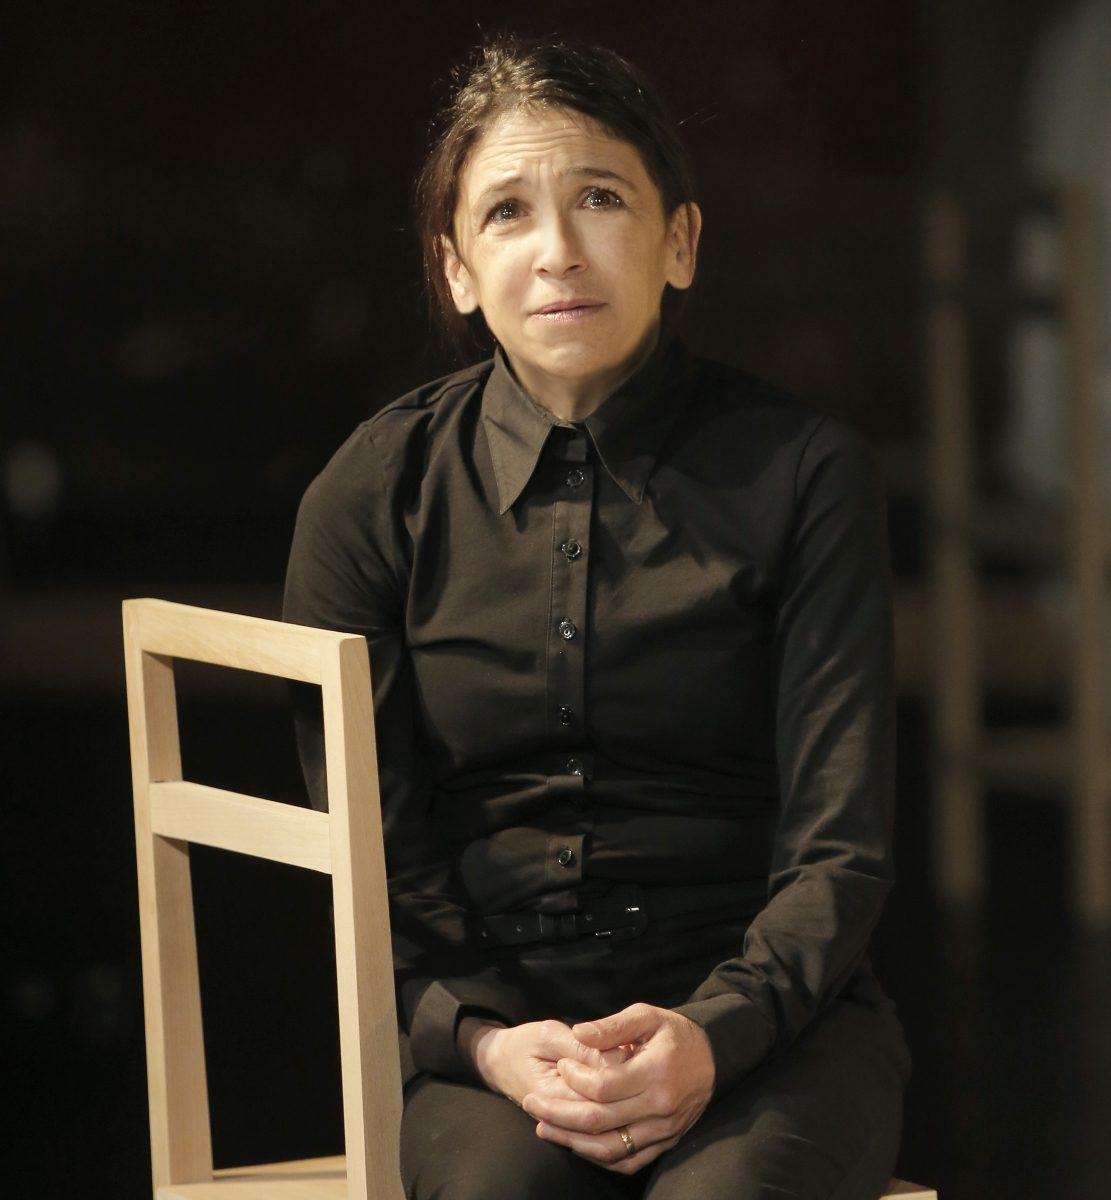
\includegraphics[width=0.5\textwidth]{./files/Kathryn-Hunter_Peter-Brook_valley-of-astonishement.jpg}
\caption{Kathryn Hunter, dans la pièce de théâtre \emph{The Valley of Astonishment}, mise en scène par Peter Brook. Le personnage est synesthète, et associe dans sa mémoire plusieurs modalités sensorielles.}
\end{figure}

\subsection{Exemples et illusions}

\subsubsection{Orientation verticale}

Prenons par exemple la perception de l'orientation haut-bas. Le système vestibulaire détecte l'accélération gravitationnelle et nous donne une information de la direction verticale et de l'orientation vers le bas. Le système visuel détecte les lignes verticales dans notre champ de vision (arbres, arêtes des murs) et distingue le ciel lumineux du sol plus sombre. Ces deux modalités sont en général cohérentes, mais on peut concevoir une salle dans lesquelles toutes les lignes sont penchées, ce qui peut perturber nos sens au point de nous faire perdre l'équilibre.

\subsubsection{Reconnaissance du langage}

Autre exemple avec la reconnaissance du langage : on comprend mieux une personne quand on la voit parler. L'information auditive du son de la voix est combinée à l'information visuelle des mouvements des lèvres et autres expressions, ce qui améliore la compréhension. Mais on peut tromper le cerveau en faisant écouter un son qui ne correspond pas au mouvement des lèvres, ce qui est alors interprété comme un autre son (cet effet connu sous le nom McGurk). 

\subsubsection{Détection d'une source sonore}

Le système auditif permet de déterminer approximativement la direction de la source d'un son grâce à l'espacement entre les deux oreilles, information qui peut être confirmée lorsque le système visuel identifie la source. Mais lorsque l'on voit un objet bouger au rythme d'un son provenant d'ailleurs, on peut lui attribuer la source du son et ignorer l'information auditive, c'est l'illusion qu'utilisent les ventriloques pour faire parler leur marionnette \cite{bonath_neural_2007}.

\subsubsection{Illusion proprioceptive}

Un exemple encore plus marquant est l'illusion proprioceptive que l'on peut déclencher avec un casque de réalité virtuelle. Dans une situation normale, le sens du toucher est combiné à l'information visuelle pour déterminer la nature des objets que l'on touche. Mais si l'on présente une main factice en image à un sujet, il peut avoir l'illusion que cette main est la sienne au point de ressentir un objet qui touche la fausse main.

\subsection{Mécanismes et échelles}

Ces multiples exemples montrent l'omniprésence de l'intégration multisensorielle dans les phénomènes perceptifs mais n'en indiquent pas les mécanismes neuronaux. Ces derniers sont complexes, avec une origine à la fois à l'échelle du neurone unique et dans l'organisation du cerveau.

\subsubsection{À l'échelle du cerveau}

Une étude en IRMf chez l'humain s'est intéressée à la structure des zones multisensorielles dans le cerveau \cite{beauchamp_unraveling_2004}. Le sujet était exposé à différents stimuli visuels (des visages) et auditifs (de voix) séparément ou combinés. Alors que les zones unisensorielles sont bien délimitées, les zones multisensorielles se sont révélées très imbriquées.
À l'échelle du cerveau en imagerie fonctionnelle par résonance magnétique, il est difficile de définir un critère sur la nature multisensorielle ou non d'une région. En effet, une étude comparant plusieurs critères statistiques montre que la superadditivité n'est pas toujours un critère pertinent dans l'étude de l'intégration multisensorielle à cette échelle \cite{beauchamp_statistical_2005}.
Alors que l'idée de cortexes sensoriels bien cloisonés était largement adoptée, une étude sur des macaques a montré que des liaisons pouvaient exister entre les différentes aires sensorielles primaires \cite{brosch_nonauditory_2005}. Une autre étude sur la gerbille a montré que le cortex auditif primaire recevait des entrées directes des cortex somatosensoriel, visuel et multisensoriel, ainsi que des structures visuelles et multisensorielles du thalamus et du tronc cérébral \cite{budinger_multisensory_2006}.
Les connexions entre les différentes régions du cerveau sont donc à la base de son fonctionnement multisensoriel. Les différentes aires sensorielles au début considérées comme unimodales se sont révélées multimodales. Les études à cette échelle tendent en effet à montrer que les différentes modalités sensorielles sont fortement liées dès un stade précoce du traitement de l'information \cite{stein_multisensory_2008}.

% The present study has shown, by use of the bidirectional
% and sensitive neuronal tracer FD, that AI of the gerbil
% (1) receives direct inputs from somatosensory, visual, and
% multisensory cortices, as well as from visual and multisen-
% sory thalamic and brainstem structures, and (2) has vari-
% ous projections to somatosensory, olfactory, visual, and
% multisensory cortical and subcortical brain regions.

\subsubsection{À l'échelle du neurone unique}

Les études à l'échelle du cerveau déconstruisent l'idée de grandes régions unisensorielles mais n'excluent pas une ségrégation des différentes modalités sensorielles à l'échelle du neurone. C'est pourquoi des études ont été menées à cette échelle plus locale. Une d'elles a révélé des connexions directes entre des neurones visuel et auditif \cite{bizley_physiological_2007} par électrophysiologie sur des furets. Dans une autre, publiée en 2007 \cite{allman_multisensory_2007}, les auteurs ont enregistré dans le cerveau de chats par électrophysiologie l'activité de milliers de neurones du sillon temporal supérieur en réponse à des stimuli visuels et auditifs combinés. Certains neurones ne répondaient qu'à un seul stimulus (neurone unimodal) alors que d'autre affichaient une réponse dans les deux cas (neurone bimodal). De plus, l'étude montre qu'il existe en proportion égales des neurones ne répondant qu'en présence des deux stimuli simultanés. Ces neurones ne seraient simplement pas détectés dans des expériences qui ne mettant en jeu qu'une seule des modalités sensorielles. À l'échelle du neurone unique, l'intégration multisensorielle se manifeste par des phénomènes tels que la super-additivité ou la sous-additivité. Certains neurones ont une réponse bien plus forte en présence de plusieurs stimuli simultanés que lorsque ceux-ci sont présentés séparément. L'amplitude de ce phénomène est d'autant plus forte que les stimuli présentent une corrélation spatiale et temporelle \cite{stein_multisensory_2008}. 

% Ces phénomènes propres à certains neurones ne sont pas présents dès la naissance et nécessitent une phase d'apprentissage.

\subsubsection{Intégration inconsciente ou interaction}

Dans une revue de 2008 \cite{angelaki_vestibular_2008}, les auteurs présentent le système vestibulaire comme particulièrement adapté à l'exploration de l'intégration multisensorielle. L'intégration multimodale a lieu très tôt dans les réseaux de neurone vestibulaires et il n'y a pas de sensation consciente du signal capté par les organes mais bien une sensation unifiée qui en résulte.
À l'opposé, certain phénomènes d'intégration peuvent avoir lieu de manière consciente, certains auteurs parlent alors d'"interaction multisensorielle" pour distinguer la manière dont plusieurs sensations interagissent entre elles d'une sensation unique résultant de l'intégration \cite{driver_multisensory_2008}. 

% We will often refer to multisensory ‘‘interplay’’ rather than
% the commonly used ‘‘integration,’’ so as to include cases where
% one modality might affect another without necessarily always im-
% plying a single unified percept.

\subsection{Le système vestibulaire chez la larve de poisson zèbre}

\subsubsection{Limites des études actuelles}

Comme nous l'avons vu, le phénomène d'interaction multisensorielle fait intervenir des neurones en petit nombre répartis dans des régions différentes du cerveau. Les études actuelles ont mis en évidence des phénomènes locaux spécifiques à certains neurones et des coactivations de régions globales à différents endroits du cerveau mais ne permettent pas d'obtenir les deux informations en même temps. 
Ces éléments montrent que l'étude de l'intégration multisensorielle doit nécessairement passer par l'analyse des réseaux entiers à l'échelle du neurone unique. Les études en IRM manquent l'échelle du neurone unique et les études d'électrophysiologie manquent les phénomènes de réseau à l'échelle du cerveau entier. C'est pourquoi un nouveau modèle qui permettent de combiner l'échelle du neurone unique et l'échelle du cerveau entier est nécessaire.

\subsubsection{Le poisson zèbre comme animal modèle adapté}

Les cerveaux de mammifères sont composés de milliards de neurones ce qui les rend trop gros pour se prêter à ce genre d'étude. C'est la raison du succès de la larve de poisson zèbre. Ce nouvel animal modèle permet, par la taille réduite de son cerveau et sa transparence de réaliser l'acquisition du cerveau entier à la résolution du neurone par des techniques d'imagerie fonctionnelle \cite{panier_fast_2013}. Cela permet l'étude de phénomènes qui ont lieu à travers tout le cerveau tout en concernant un petit nombre de neurone. Le poisson zèbre partage la structure de son cerveau avec les autres vertébrés tout en ayant un catalogue de comportement assez riche. De nombreuses études concernant ses différentes modalités sensorielles et leur bases neuronales ont été publiées depuis 2013. Comme cité plus haut, le modèle vestibulaire se prête bien à l'étude de l'intégration multisensorielle, c'est donc le système que nous avons choisi d'étudier.


\section{Imagerie fonctionnelle par microscopie à feuille de lumière}

\subsection{Comment enregistrer le cerveau entier ?}

Comme nous l'avons vu, les techniques d'acquisition de l'activité neuronale comme l'électrophysiologie et l'imagerie par résonance magnétique ne sont pas adaptées pour réaliser l'imagerie du cerveau entier à l'échelle du neurone unique. Il est donc nécessaire d'utiliser une technique d'acquisition non invasive capable de telles performances. Travailler sur un animal transparent comme la larve de poisson zèbre facilite l'acquisition utilisant la lumière visible, c'est-à-dire l'imagerie optique. Celle-ci est très développée en biologie et peut assurer à la fois une bonne résolution et un champ large. Cependant, plusieurs innovations importantes à la fois en optique, en ingénierie moléculaire, et en génétique ont dû être combinées pour arriver à un tel résultat. Nous l'introduisons ici.

\subsection{Imagerie fonctionnelle calcique}

\subsubsection{Architecture et fonctionnement du neurone}

Le neurone est une cellule fortement présente dans le cerveau et caractérisée par son prolongement axonal capable de transmettre un influx nerveux. Il est toujours accompagné par des cellules gliales comme les astrocytes ou les oligodendrocytes qui assurent en grande partie les fonctions métaboliques. Il est aujourd'hui considéré comme principal responsable des processus cognitifs bien que de nombreuses recherches montrent l'importance des cellules gliales dans des phénomènes tels que l'intégration du signal calcique et l'établissement de connexions synaptiques \cite{verkhratsky_calcium_1996} \cite{pfrieger_synaptic_1997}.

\begin{figure}
\centering
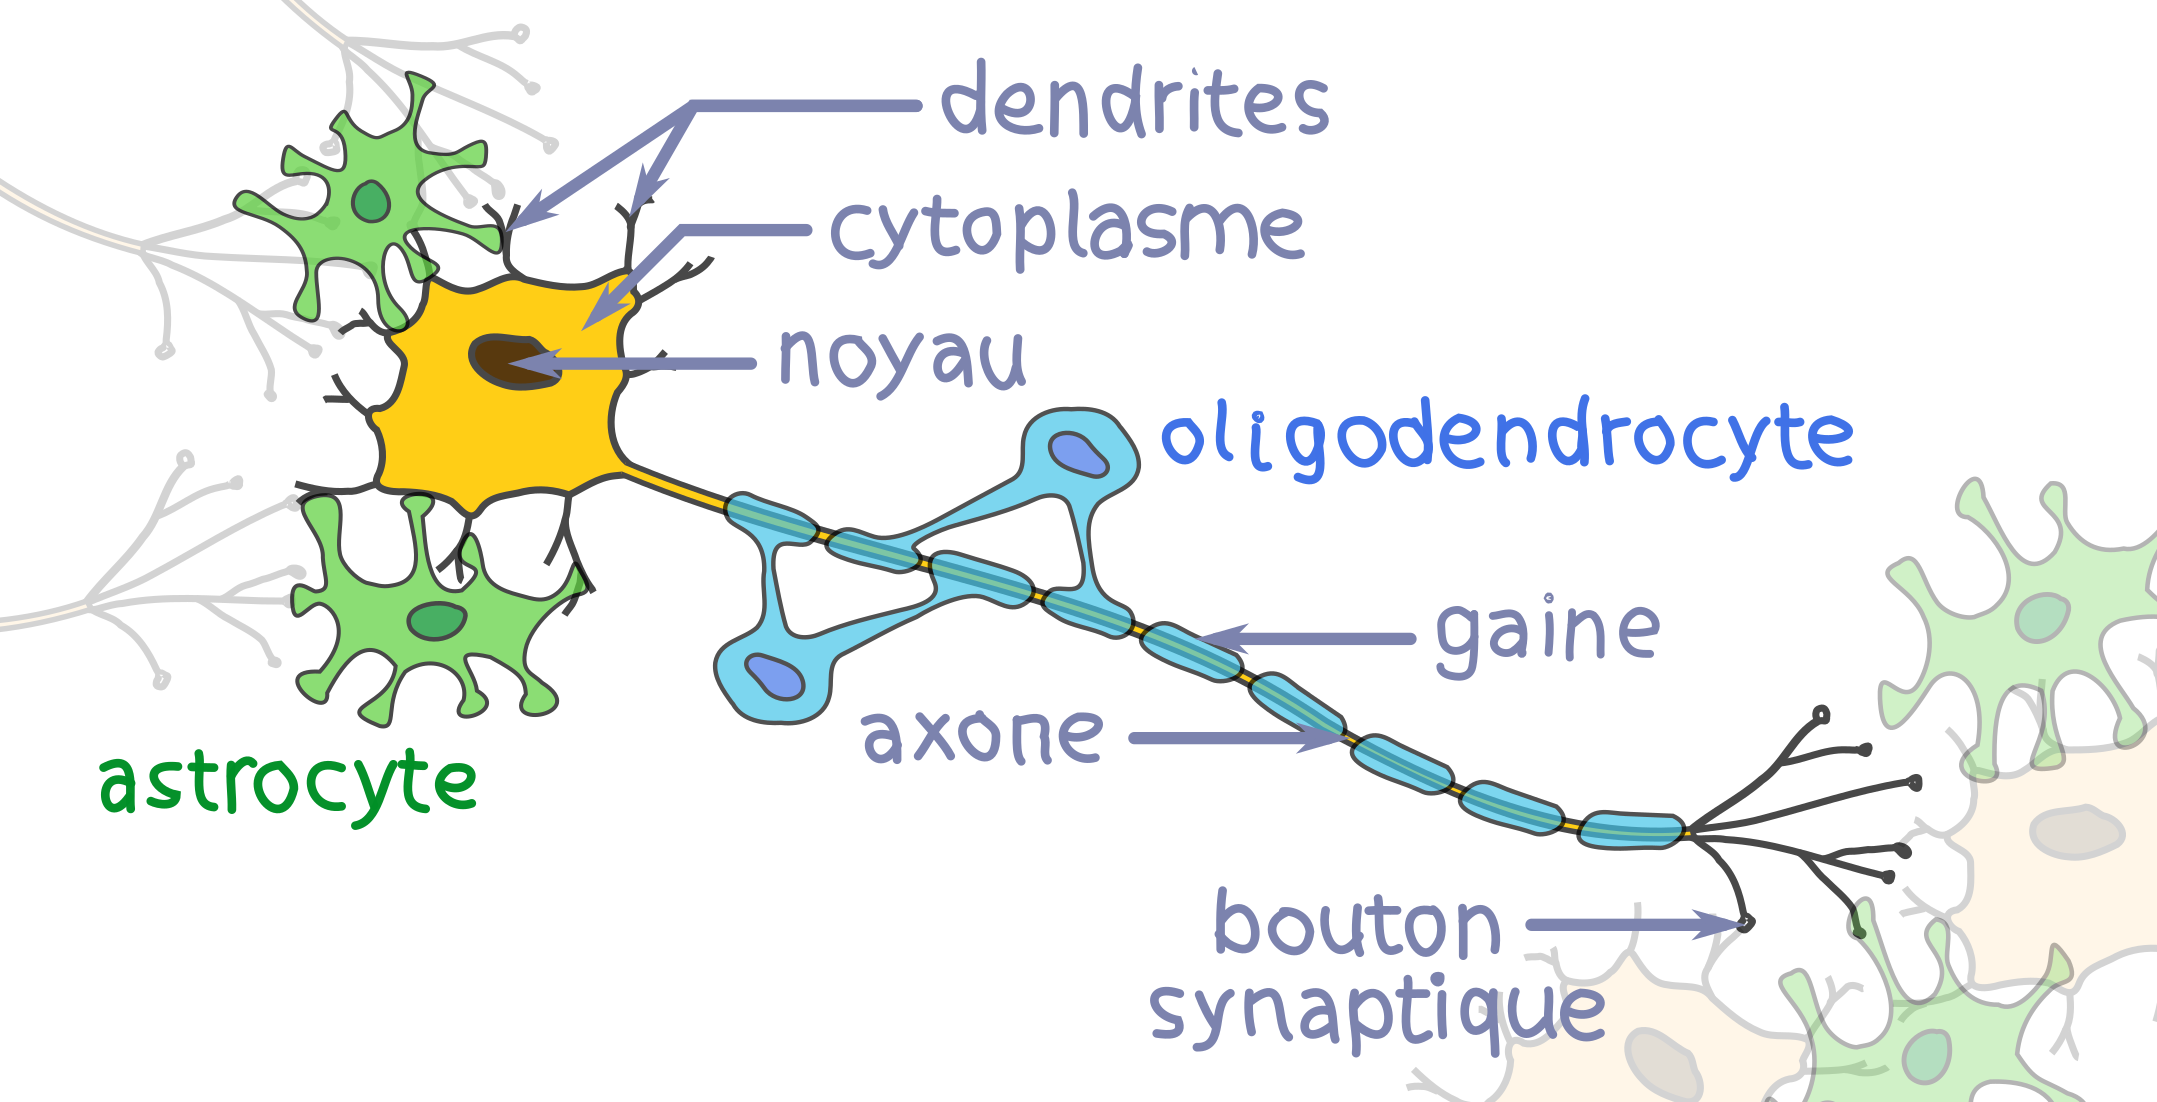
\includegraphics[width=0.8\textwidth]{./files/neurone.svg.png}
\caption{Schéma d'un neurone accompagné de cellules gliales. Astrocytes (en vert), oligodendrocytes (en bleu). Le neurone dispose d'un long prolongement appelé axone qui le connecte à d'autres neurones via des boutons synaptiques.}
\end{figure}

Le neurone est doté d'une longue projection nommée axone, qui lui permet de se connecter et transmettre un signal à d'autres neurones éloignés de lui. Comme la plupart des cellules, des protéines transmembranaires lui permettent d'atteindre une différence de potentiel avec l'extérieur de -70 mV au repos et comme d'autres cellules dites excitables, cela lui permet de transmettre un signal électrique par ouverture et fermeture de canaux ioniques.

\subsubsection{Le calcium dans le neurone}

Le neurone est équipé de pompes et canaux ioniques sur sa membrane qui lui permettent de se polariser en faisant varier la concentration d'ions intracellulaires par rapport au milieu extracellulaire. Ce potentiel électrochimique transmembranaire varie brusquement lors d'événements de dépolarisation qui permettent la propagation d'un message le long des projections axonales vers d'autres neurones. Lors de ces événements, des flux d'ions traversent la paroi cellulaire, ce qui modifie largement leur concentration intracellulaire. Par exemple, l'ion calcium ($Ca^{2+}$) passe d'une concentration de 0.1 µmol/L à 10 µmol/L soit un facteur 100 \cite{grienberger_imaging_2012}, la concentration extracellulaire étant de 1 mmol/L, encore cent fois plus. La durée des potentiels d'actions est de l'ordre de la milliseconde, et la concentration de calcium évolue sur des échelles de temps similaires, de l'ordre de la dizaine de millisecondes [?].

\begin{figure}
\centering
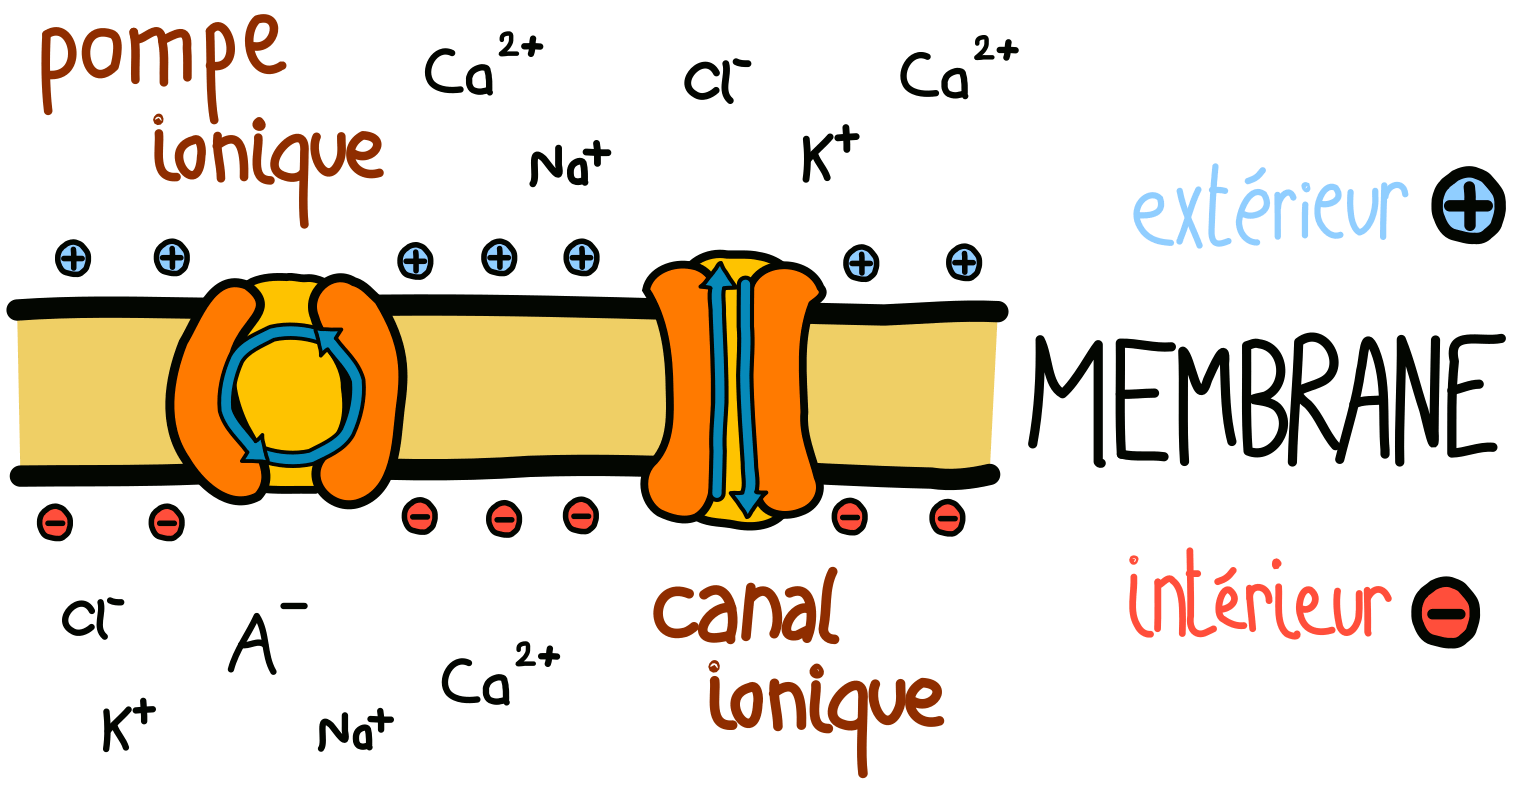
\includegraphics[width=0.8\textwidth]{./files/membrane.svg.png}
\caption{Des protéines transmembranaires permettent à la cellule de se polariser et de se dépolariser. Les pompes ioniques consomment de l'énergie sous forme d'ATP pour forcer le passage d'ions. Des transporteurs ioniques actifs (symport, antiport) et passifs (uniport) permettent un transport dirigé d'ions. Des canaux sélectifs et non sélectifs permettent un transport rapide.}
\end{figure}

\subsubsection{GCaMP, rapporteur calcique}

Du fait de ses grandes variations de concentration, l'ion calcium est un bon indicateur des potentiels d'actions et donc de l'activité neuronale. C'est la raison pour laquelle des rapporteurs calciques ont été développés. Parmi eux, le rapporteur encodé génétiquement GCaMP résulte de l'assemblage entre la calmodulin (calcium modulated protein), une protéine qui se lie au calcium ce qui change sa conformation, et d'une protéine fluorescente verte (GFP, \emph{Green Fluorescent Protein}). Le résultat est une protéine qui devient fluorescente en présence d'ion calcium, avec une dynamique de l'ordre du dixième de seconde. Le code génétique de cette protéine peut être inséré dans une région d'intérêt du génome, pour être exprimée dans des populations ciblées de neurones.

\begin{figure}
\centering
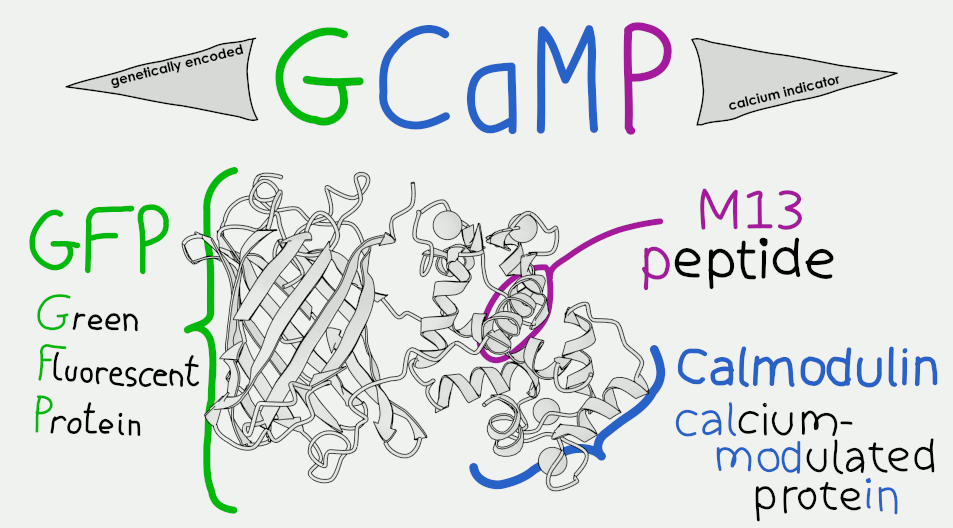
\includegraphics[width=0.8\textwidth]{./files/GCaMP.png}
\caption{Structure tridimensionnelle de l'indicateur calcique GCaMP composée de trois ensembles protéiques.}
\end{figure}

Ainsi, l'organisme génétiquement modifié est équipé d'une molécule présente dans les neurones dont la fluorescence varie en fonction de l'activité du neurone. Cela permet de réaliser l'imagerie fonctionnelle, c'est-à-dire l'imagerie des cellules lors de leur fonctionnement, par l'observation des modifications de leur métabolisme aux échelles de temps courtes. 

\subsection{Microscopie à fluorescence et feuille de lumière}

\subsubsection{Principe de la microscopie}

Le principe général d'un microscope optique est d'éclairer un échantillon et d'observer la lumière qui rentre dans le système de détection. Sur un échantillon mince, on peut faire de la microscopie en transmission ou en réflexion, mais pour un échantillon biologique épais, le phénomène de diffusion rend ces techniques inutilisables. Lorsque le volume imagé est prédéfini, par exemple en imagerie médicale, il faut se contenter de l'auto-fluorescence et élaborer des techniques sophistiqués pour repousser les limites de la diffusion. Au contraire, lorsque l'on contrôle le volume à imager, il est possible de réaliser un marquage fluorescent qui permet de cibler un sous-ensemble précis du tissu biologique et d'émettre autour d'une longueur d'onde choisie.

\subsubsection{Fluorescence}

La fluorescence est un phénomène d’absorption-réémission de lumière par une molécule. Dans le cas de GFP (ainsi que GCaMP), la protéine absorbe les longueurs d'onde dans le bleu et émet dans le vert. Il est ainsi possible de stimuler la fluorescence en utilisant un laser à 488 nm (en imagerie un photon) et de collecter la lumière ré-émise. 

\begin{figure}
\centering
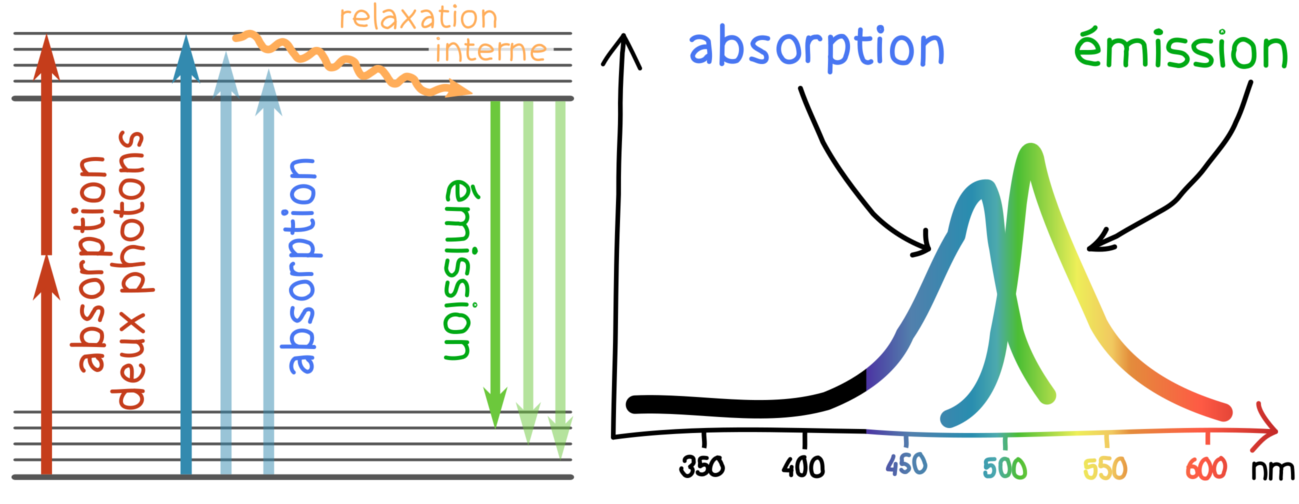
\includegraphics[width=0.8\textwidth]{./files/fluo_couleur.svg.png}
\caption{Illustration du phénomène de fluorescence. À gauche point de vue quantique avec les niveaux d'énergie interne, à droite point de vue ondulatoire avec les spectres d’absorption et d'émission}
\end{figure}

Un des avantages de la microscopie à fluorescence est qu'avec un jeu de filtres adapté, on peut obtenir un excellent rapport signal à bruit. Ainsi, en plaçant sur la ligne de détection un filtre coupe bande à la longueur d'onde du laser, on peut couper toute lumière venant de celui-ci. En ajoutant un filtre passe bande vert, seule la lumière liée à la fluorescence est détectée.

\subsubsection{Sectionnement optique}

Si l'on éclaire l'ensemble d'un échantillon fluorescent et que l'on tente de l'imager avec un objectif de microscope, le rapport signal à bruit est catastrophique. En effet, pour collecter le maximum de lumière, il faut une grande ouverture numérique et donc une faible la profondeur de champ. Un objet lumineux hors du plan focal apparaît donc totalement flou, ce qui constitue une lumière parasite qui couvre celle émise par les objets dans le plan focal. Il faut donc d'une manière ou d'une autre éliminer la lumière provenant d'en dehors du plan focal.

\begin{figure}
  \centering
  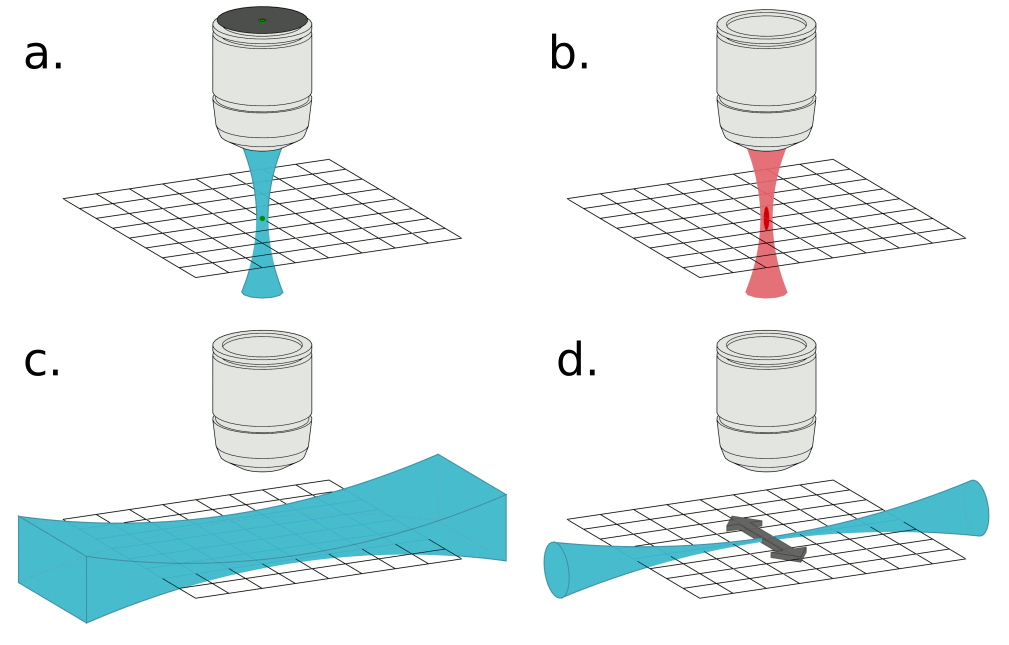
\includegraphics[width=0.8\textwidth]{./files/optical_sectionning.svg.png}
  \caption{Sectionnement optique par différentes techniques \\
  a. Microscopie confocale, un sténopé est placé de manière à bloquer la lumière provenant des points hors focus. \\
  b. Microscopie deux photons, l'effet deux photons permet d'exciter uniquement la fluorescence dans le point de focalisation du laser. \\
  c. Feuille de lumière, une nappe produite avec une lentille cylindrique éclaire une couche de l'échantillon. \\
  d. Balayage laser, une nappe produite par balayage laser éclaire une couche de l'échantillon. \\
  }
  \end{figure}

\subsubsection{Microscopie confocale}

Il existe pour cela plusieurs techniques dites de "sectionnement optique". La plus connue, la microscopie confocale, utilise une illumination focalisée en un seul point. L'objet en ce point est donc fortement éclairé, et le reste beaucoup moins. De plus, un sténopé conjugué à ce point ne laisse passer que la lumière qui en est issue. L'imagerie d'un plan est ensuite obtenue en scannant ce point dans le plan focal, et l'imagerie d'un volume et répétant l'opération pour plusieurs couches. Cette technique est largement répandue et déclinée, et a l'avantage d'être souple et d'atteindre de bonnes résolutions. Cependant, elle ne peut pas combiner une haute définition ($\sim 10^8$ voxels) à une fréquence élevée ($\sim 1$ Hz) et doit sacrifier l'un pour l'autre. Elle est donc réservée soit à l'observation détaillée d'échantillons statiques, soit à l'observation peu détaillée d'échantillons dynamiques. Cette lenteur est liée au fait de scanner un point sur une surface, mais on peut gagner en vitesse au détriment du rapport signal à bruit en éclairant une ligne d'un coup et en remplaçant le trou par une fente, car il suffit alors de scanner dans une seule dimension.

\subsubsection{Microscopie deux photons}

La microscopie deux photons utilise une propriété non linéaire de la lumière pour exciter la fluorescence uniquement en un point. De manière analogue à la microscopie confocale, un faisceau est concentré en un point de l'échantillon, mais l'utilisation d'un laser pulsé dans l'infrarouge permet d'atteindre des niveaux de puissance instantanée bien plus élevés tout en pénétrant mieux les tissus biologiques. De plus, l'utilisation d'un sténopé n'est pas nécessaire car l'effet deux photons est proportionnel au carré de l'intensité lumineuse, et seul le point de focalisation est donc excité. Comme la microscopie confocale, il s'agit alors de scanner un point à travers tout l'échantillon, ce qui est trop lent pour l'imagerie de grands volumes.  

\subsubsection{Microscopie à feuille de lumière}

En microscopie confocale ou deux photons, l'illumination passe par le même objectif que la détection. Mais pour certains échantillons, l'éclairage peut également être fait par le côté. Une feuille de lumière coïncidant avec le plan focal de l'objectif peut être produite à l'aide d'une lentille cylindrique, ou bien par balayage d'un faisceau laser. C'est ce qu'on appelle la microscopie à feuille de lumière, microscopie à nappe laser, ou encore SPIM pour \emph{Single Plane Imaging Microscopy}. Cette technique, en dépit d'un rapport signal à bruit et d'une résolution inférieurs à la microscopie confocale, suffit pour réaliser l'imagerie à la résolution cellulaire. De plus, elle permet d'imager un plan entier d'un seul coup, ce qui est bien pus rapide. En scannant l'objectif et la feuille de lumière, on peut ainsi produire une imagerie volumique à fréquence bien plus élevée qu'en microscopie confocale. Par exemple, avec trente couches espacées de dix microns, on peut acquérir l'ensemble du cerveau d'une larve de poisson zèbre à environ 2Hz.

Si la microscopie par fluorescence à feuille de lumière est une technique particulièrement adaptée à la bio-imagerie fonctionnelle, son utilisation reste toutefois relativement faible. En 2011, un article de revue pointait le manque de système commercial en microscopie à feuille de lumière \cite{santi_light_2011}. En 2017, un autre déplorait le faible niveau de propagation de cette technique au regard de ses performances \cite{power_guide_2017}. La technique reste donc cantonnée à des laboratoires capables de développer leur propre microscope en dépit du succès qu'elle rencontre dans ses applications.



\section{Intégration multisensorielle chez la larve de poisson zèbre}

La microscopie à feuille de lumière permet d'enregistrer le cerveau entier d'une larve de poisson zèbre à la résolution du neurone et avec une fréquence de quelques Hertz. Plusieurs études ont mis en œuvre cette technique pour étudier différents aspects du fonctionnement du cerveau. Je m'intéresse ici aux stratégies mises en œuvre pour étudier l'intégration multisensorielle pour étudier la boucle sensorimotrice, et plus particulièrement sur le modèle visuo-vestibulaire.

% TODO séparer comportement / étude neuronale

\subsection{Boucle sensorimotrice}

Une capacité intéressante du cerveau est le fonctionnement en boucle fermée. En effet, à la manière d'un système d'asservissement, il est capable de mesurer un paramètre extérieur, le comparer à une valeur de commande et agir pour le contrôler. Par exemple, lorsqu'un poisson est emporté par le courant d'une rivière, il détecte un flux optique sous lui et déclenche la nage. Le flux optique résultant est alors la somme de la vitesse du poisson par rapport au fluide et de la vitesse du fluide par rapport au sol. Ce flux optique mesuré permet au poisson d'évaluer si sa nage est efficace pour compenser le courant, s'il doit nager plus vite ou moins vite. Beaucoup des réflexes sont en fait des boucles sensorimotrices dans lesquelles les entrées sensorielles servent en permanence à évaluer la sortie motrice. Deux options se présentent pour étudier ces boucles sensorimotrices. L'une est l'étude en nage libre, l'autre est l'étude en environnement virtuel avec rétroaction.

\subsubsection{Imagerie en nage libre}

Une option pour étudier le poisson dans son environnement naturel est de construire un microscope motorisé capable de suivre les mouvements du poisson lors de la nage de manière à toujours pouvoir imager le cerveau. C'est l'approche adoptée par le laboratoire RoLi \cite{kim_pan-neuronal_2017} qui peut ainsi observer certains comportements difficiles à reproduire avec un poisson immobilisé. L'illumination par le côté étant impossible dans ce cas, c'est une technique de microscopie structurée développée par Jérôme Mertz \cite{mertz_optical_2011} qui a été utilisée.

\subsubsection{Réalité virtuelle}

Une autre option pour étudier la boucle sensorimotrice est de reproduire en environnement virtuel pour simuler la boucle de rétroaction sensorimotrice. Un stimulus sensoriel est soumis au poisson qui réagit en fonction. Sa réponse est mesurée et répercutée sur l'environnement virtuel d'une manière fidèle à la réalité ou volontairement biaisée.

\paragraph{Adaptation motrice fictive}
Ahrens \emph{et al} ont étudié la boucle sensorimotrice dans le cas de l'OMR \cite{ahrens_brain-wide_2012}. Ils ont pour cela créé un environnement fictif dans lequel une larve paralysée est placée au-dessus d'un écran. Des bandes mobiles sont présentées au poisson, ce qui déclenche le réflexe optomoteur. L'activité des neurones moteurs est enregistrée à l'aide d'électrodes (les muscles sont inactifs, car le poisson est paralysé), et ce signal est utilisé pour simuler un déplacement par un mouvement des bandes en sens opposé. Dans cet environnement virtuel, ils ont pu tester des mécanismes comme l'adaptation de gain tout en enregistrant l'activité des neurones. Cela a permis d'identifier les neurones responsables de l'augmentation du gain et de la diminution du gain, qui sont essentiels pour le fonctionnement de la boucle de rétroaction.

\paragraph{Sans rétroaction, comportement d'abandon} % TODO reformuler
Dans le même article \cite{ahrens_brain-wide_2012}, les auteurs ont testé le comportement du poisson dans un système en boucle ouverte, c'est-à-dire sans rétroaction. Les bandes mobiles sont présentées au poisson à vitesse constante sans prendre en compte l'activité des neurones moteurs. Dans cette situation, le comportement de nage est inhibé malgré la présence de stimulus. Cette inhibition due à l'absence de rétroaction peut durer une dizaine de secondes, même après la remise en marche de la rétroaction. Cela montre l'importance du rétrocontrôle dans le fonctionnement de la boucle sensorimotrice et la nécessité d'un système en boucle fermée pour son étude. 

% \paragraph{TODO OKR ?}

% TODO Portugues 2014 Whole-Brain Activity Maps Reveal Stereotyped, Distributed Networks for Visuomotor Behavior

% \paragraph{TODO rhéotaxis ?}

% TODO Oteiza 2017 A novel mechanism for mechanosensory-based rheotaxis in larval zebrafish

% * setups existants pour autres modalités sensorielles
%   * rétroaction système visuel (Portuguese, Ahrens)
% * comment stimuler le système vestibulaire ?
%   * pinces optiques (ne pas parler de pinces magnétiques)
%   * plateforme rotative


\subsection{Modèle viso-vestibulaire}

Un terrain idéal pour étudier l'intégration multisensorielle est le modèle visuo vestibulaire. Ces deux modalités sensorielles sollicitées de concert lors de la nage pour la stabilisation de la posture et de la vision sont pratiquement développées chez la larve de six jours. En effet, le système visuel est fonctionnel dès 4 jours \cite{bollmann_zebrafish_2019}, et le système vestibulaire dès 5 jours (seulement l'utricule) \cite{haddon_early_1996}. Mais avant de décrire les réflexes qui mettent en jeux ces deux modalités sensorielles simultanément, intéressons-nous séparément à l'appareil visuel et à l'appareil vestibulaire.

\subsubsection{Système visuel}

\paragraph{Organisation}
La partie neuronale du système visuel commence par une rétine munie de cellules qui captent la lumière. La répartition des capteurs en fonction de leur couleur correspond aux teintes rencontrées dans l'habitat naturel du poisson. Des circuits neuronaux dans la rétine réalisent un pré-traitement qui, bien qu'en pleine évolution chez une larve de six jours, lui permet déjà de réaliser des opérations complexes. Par exemple, certaines cellules ganglionnaires rétiniennes sont sensibles à l'orientation de motif ou à la direction de mouvement d'un objet, d'autres à la taille d'un objet ou à son évolution \cite{bollmann_zebrafish_2019}. L'étude de l'arborescence de ces ganglions révèle plusieurs zones spécifiques à certains stimuli, comme des variations globales de luminance, le mouvement de petits objets, des déplacements sur tout le champ de vision... La plupart de ces ganglions projettent vers le tectum optique (équivalent du colliculus supérieur chez l'humain) où la suite du traitement est effectuée à travers sa structure laminaire.

\cite{portugues_neural_2009}

\paragraph{OMR, réponse optomotrice}
Certains comportements comme l'OMR (\emph{optomotor response}, réponse optomotrice) et l'OKR (\emph{optokinetic response}, réponse optocinétique) sont purement liés au système visuel. L'OMR est un comportement qui survient de manière très reproductible lors d'un mouvement de translation global dans l'ensemble du champ de vision. La larve se met à nager à l'encontre du flux optique rencontré. Dans la nature, ce comportement permet de compenser le courant d'une rivière pour rester au même niveau en se servant de l'environnement visuel comme référence. En laboratoire, on peut facilement reproduire ce comportement en projetant un motif en translation sous la larve, ce qui provoque des mouvements de queue.

\paragraph{OKR, réponse optocinétique}
L'OKR est un mécanisme de stabilisation de la vision dans lequel l’œil compense les mouvements globaux de l'environnement pour en conserver une vision nette. Cette réponse peut également être étudiée facilement en laboratoire en présentant un motif mobile sur un écran face à une larve. Ces deux comportements sont importants dans l'étude des réponses aux stimulations vestibulaires en présence d'un environnement lumineux. En effet, une accélération ou une rotation de la larve entraîne mécaniquement un mouvement global de l'environnement visuel de celle-ci.

\subsubsection{Système vestibulaire}

\paragraph{Organisation}
L'organe vestibulaire, quant à lui, est situé dans l'oreille interne. Grâce à des cellules ciliées sensibles à leur propre déflexion, il peut mesurer les accélérations inertielle et gravitationnelle auxquelles sont soumises les otolithes (petites pierres osseuses) et les accélérations angulaires du liquide présent dans les canaux semi-circulaires. Bien que quasiment mature chez la larve dès cinq jours, la taille des canaux semi-circulaires les rend inefficaces et donc seule l'utricule (un des otolithes) est fonctionnel. Cela est cependant suffisant (et nécessaire \cite{riley_development_2000}) pour que la larve puisse nager tout en conservant son équilibre.

\begin{figure}
\centering
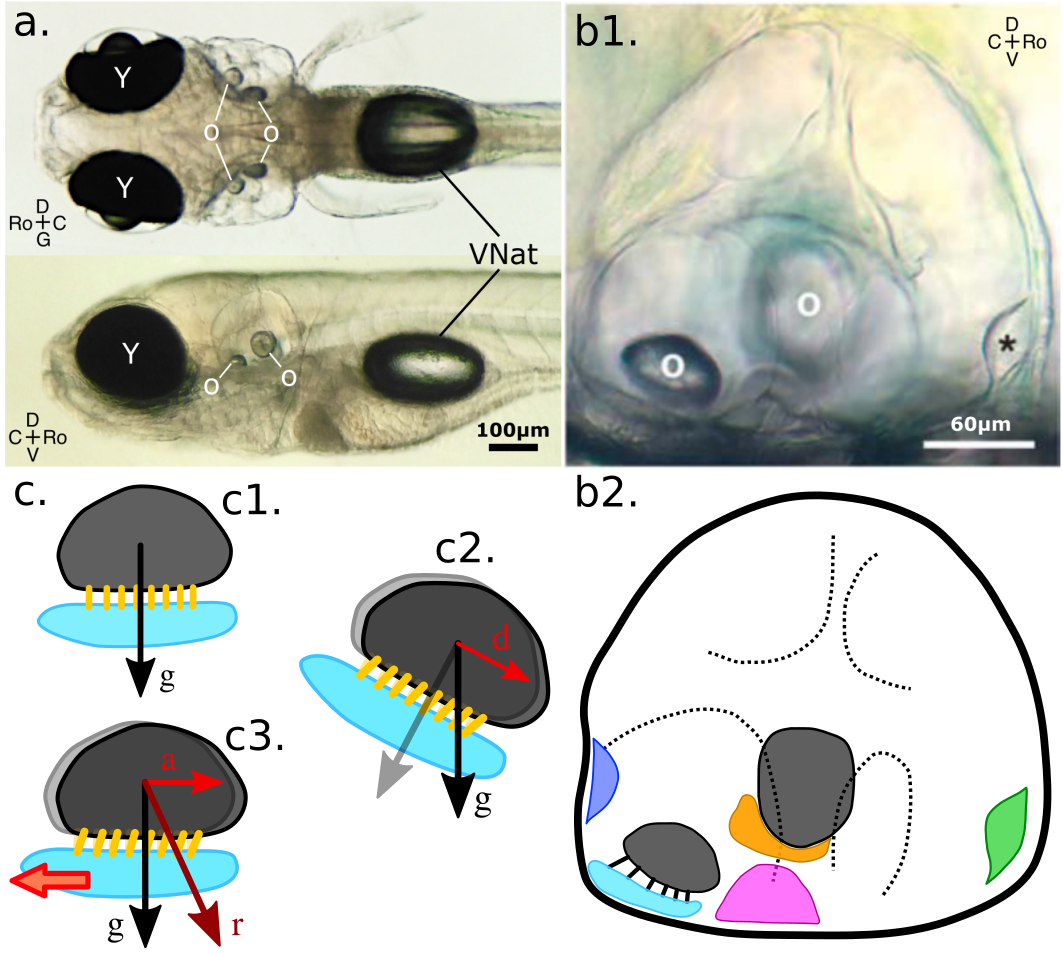
\includegraphics[width=0.6\textwidth]{./files/appareil_vestibulaire.svg.png}
\caption{
Schéma adapté de G. Migault
\\
A. Larve de poisson zèbre de 6 jours vue de dessus (haut) et de côté (bas). On distingue les yeux (Y), l'oreille interne avec ses otolithes (O) et la vessie natatoire (VNat).
\\
B. Agrandissement de l'oreille interne vue de côté (B1) avec le schéma correspondant (B2). On souligne en pointillé les canaux semi-circulaires, en gris les deux otolithes, et en couleur les neuro-épithéliums.
\\
C. Otolithe en fonctionnement. Lorsqu'il est à l'horizontale (C1), les cils sont au repos, lorsqu'il est incliné (C2), les cils sont défléchis car l'accélération gravitationnelle change de direction, lorsqu'il est en mouvement accéléré vers la gauche (C3), l'accélération inertielle (a) s'ajoute à l'accélération gravitationnelle (g) et donne la résultante (r). On voit que l'utricule ne permet pas de différencier l'accélération gravitationnelle de l'accélération inertielle.}
\end{figure}

Les neurones répondant aux stimulations vestibulaires sont présents à de nombreux endroits du cerveau, à la fois dans le prosencéphale (télencéphale, habenulae, thalamus, prétectum), dans le mésencéphale (tectum, nMLF, tegentum), et dans le rombencéphale (cervelet, MON, rhombomère 5-7) \cite{favre-bulle_cellular-resolution_2018}. Chacune de ces régions est impliquée différemment dans les réflexes vestibulaires comme le réflexe vestibulo-oculaire (\emph{vestibulo-ocular reflex}, VOR) et le contrôle postural où réflexe vestibulo-spinal (\emph{vestibulo-spinal reflex}, VSR).

\paragraph{VOR, réflexe vestibulo-oculaire} \label{VOR}
Le VOR, largement répandu chez les vertébrés et également observé chez le poisson-zèbre \cite{bianco_tangential_2012}. C'est un mouvement réflexe des yeux qui compense les mouvements de la tête pour stabiliser la vision. Bianco \emph{et al} l'ont mis en évidence chez la larve de poisson zèbre de plus de 4 jours en la soumettant à une rotation selon l'axe de tangage, ce qui génère une rotation des yeux opposée, avec un angle limité par le maximum physiologique. Le circuit neuronal associé est constitué d'un neurone afférent primaire, un neurone vestibulaire de second ordre, et un motoneurone oculaire qui guide la rotation de l’œil. Ce circuit est présent en deux exemplaires avec une symétrie bilatérale, pour chacun des utricules. Il a également été montré que les neurones du noyau tangentiel ont des projections dans les motoneurones oculaires contra-latéraux, et que ces neurones sont essentiels au fonctionnement du réflexe. 

\paragraph{VSR, réflexe vestibulo-spinal} \label{VSR}
Le VSR est un réflexe de contrôle de posture qui utilise également l'information vestibulaire. Chez le poisson zèbre adulte, la vessie natatoire est un organe important qui permet de contrôler la flottaison, mais chez la larve, elle n'est pas encore fonctionnelle. Les effecteurs du contrôle postural sont donc surtout la queue et les nageoires. Ehrlich \emph{et al} ont étudié le déséquilibre naturel de la larve en \emph{tangage} et ont montré que les événements de nage sont à la base du développement de l'équilibre \cite{ehrlich_control_2017}. Favre-Bulle \emph{et al} ont étudié le contrôle de l'équilibre dans l'axe de \emph{roulis} en stimulant directement les utricules dans l'oreille interne et ont constaté une déflexion proportionnelle de la queue \cite{favre-bulle_cellular-resolution_2018}.

\subsubsection{Intégration viso-vestibulaire}

Les quatre réflexes cités précédemment peuvent être isolés en laboratoire, en contrôlant séparément la stimulation visuelle et la stimulation vestibulaire, mais en réalité, ces réflexes sont très intriqués. En effet, le OKR et le VOR contrôlent tous les deux le mouvement des yeux alors que l'OMR et le VSR contrôlent tous les deux le mouvement de la queue et des nageoires. Dans certains cas, ils peuvent jouer dans le même sens (stimulations cohérentes) alors que dans d'autres ils peuvent entrer en conflit (stimulations incohérentes). C'est précisément cette interaction entre les deux modalités sensorielles qui nous intéresse, et c'est également la raison pour laquelle le système vestibulo-oculaire se prête particulièrement bien à l'étude des stimulations multimodales. Une première étude montre comment dans certains cas, l'information visuelle peut moduler les rotations de l'œil induites par l'utricule \cite{bianco_tangential_2012}.


\section{Objectifs de la thèse}

% TODO Volker (objectifs thèse)
% Open question. Hypotheses. Outline your personal thesis work and results

Les objectifs de ma thèse ont été d'une part de reproduire la boucle sensorimotrice du contrôle postural dans un environnement virtuel, et d'autre part de réaliser un montage capable d'acquérir l'activité neuronale lors de stimulations visuelle et vestibulaire simultanées.
\chapter{Contrôle postural dans un environnement virtuel}\label{chapII}

La larve de poisson zèbre est fondamentalement déséquilibrée. Son centre de gravité est décalé vers l'avant par rapport à son centre de flottaison, ce qui la fait piquer du nez dans l'axe de tangage. Une larve paralysée se retrouve sur le flanc dans l'axe de roulis. C'est donc par un contrôle permanent qu'elle se maintient à l'horizontale. Pour cela, elle utilise à la fois les informations visuelle et vestibulaire pour déclencher des mouvements de queue et de nageoires qui la stabilisent. Ces comportements complexes ont été étudiés en nage libre par David Ehrlich et David Schoppik, mais pour comprendre les mécanismes neuronaux à l'œuvre, il est nécessaire de fixer le poisson sous un objectif de microscope. J'ai donc cherché à reproduire ces comportements dans un environnement virtuel en vue d'une étude sous microscope.

\section{Description de la boucle sensorimotrice}

La larve de poisson zèbre évolue dans un environnement en trois dimensions. Elle peut se déplacer suivant les trois degré de liberté en translation et s'orienter suivant les trois degrés de liberté en rotation. Certains comportements comme la thigmotaxie (affection pour les bords) sont liés à sa position dans son environnement, mais dans le cadre du contrôle postural, on s'intéresse surtout à deux degrés de rotation que sont le roulis et le tangage.

\begin{figure}
\centering
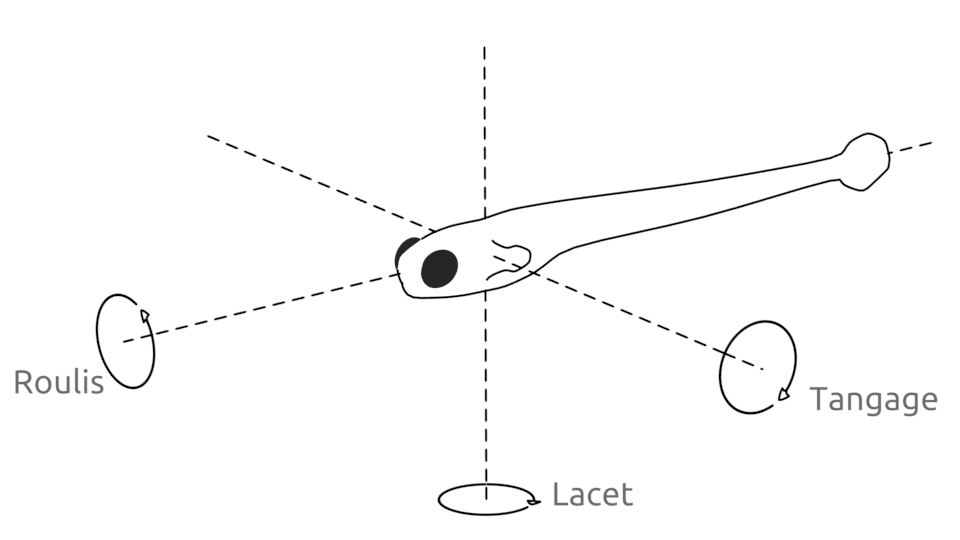
\includegraphics[width=0.8\textwidth]{./files/fish.png}
\caption{Larve de poisson zèbre dans sa position naturelle. Cette position est hors équilibre, un poisson inactif tourne sur l'axe de roulis et de tangage.}
\end{figure}

\subsection{Roulis}
Dans l'axe de roulis, la larve contrôle son équilibre par des déflexions de la queue. Si elle penche trop à gauche, elle bascule sa queue vers la droite, un peu comme un humain utiliserait ses bras pour s'équilibrer. Le contrôle postural en roulis se fait donc par une boucle de rétroaction sensorimotrice continue. L'angle de référence est de 0°, l'organe vestibulaire mesure l'écart à cet angle, et la queue le compense par une déflexion opposée. Ce comportement a été observé par Favre-Bulle \emph{et al} en simulant une rotation via une manipulation de l'utricule dans l'oreille interne par des pinces optiques. Cette étude a été réalisée en boucle ouverte, c'est-à-dire sans rétroaction, ce qui fait que la larve ne pouvait pas constater les effets de son mouvement. Une expérience de réalité virtuelle en rétroaction pourrait simuler un déséquilibre proportionnel à l'angle de la queue, ce qui permettrait à la larve d'en corriger l'angle en temps réel.

\subsection{Tangage}
Dans l'axe de tangage, la situation est plus compliquée. L'angle que fait la larve avec l'horizontale dépend de sa direction de déplacement. Par exemple, une larve se place à un angle positif lorsqu'elle nage vers le haut pour remonter à la surface et un angle négatif quand elle nage vers le bas \cite{ehrlich_primal_2019}. Cet angle constitue une référence autour de laquelle la larve cherche à se stabiliser. Ehrlich et Schoppik ont montré que le contrôle de l'angle se faisait exactement pendant les mouvements de nage \cite{ehrlich_control_2017}. La larve de poisson zèbre nage de manière discrète via des mouvements réguliers à une fréquence d'environ un par seconde en nage libre. Entre deux mouvements, elle est soumise à son déséquilibre et son nez tombe à une vitesse déterminée par sa morphologie. Lors d'un mouvement, en fonction de la force et la position des nageoires, l'angle augmente d'un coup. De plus, les auteurs suggèrent que l'initiation du mouvement est induite par l'angle ressenti. Ils ont augmenté artificiellement le déséquilibre de la larve, conduisant à une chute plus rapide. Ils ont constaté que la larve compensait ce déséquilibre supplémentaire par une augmentation de la fréquence des mouvements de nage.
Le contrôle postural en tangage est donc le résultat d'une boucle de rétroaction sensorimotrice discrète. L'angle de référence varie entre -15° et +20° environ et dépend de la direction souhaitée par le poisson. L'action de contrôle de l'angle implique à la fois la queue et les nageoires et se fait au moment des événements de nage, dont la fréquence peut être ajustée en fonction du déséquilibre.

\begin{figure}
\centering
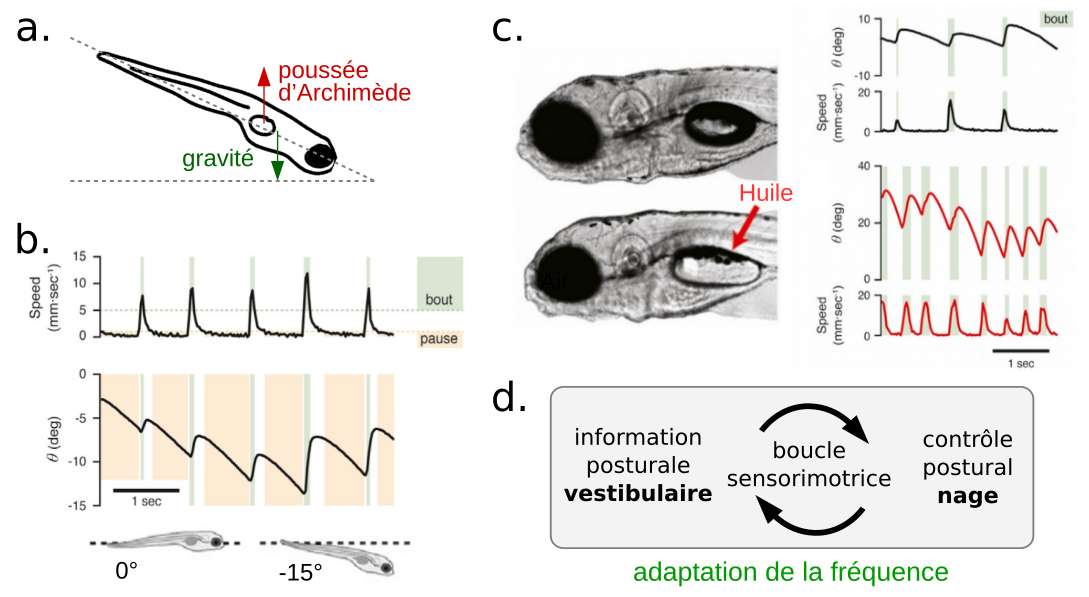
\includegraphics[width=0.8\textwidth]{./files/schoppik_movement-initiation.svg.png}
\caption{Adapté de Ehrlich et al \cite{ehrlich_control_2017}
\\
a. Le centre de gravité et de flottaison de la larve sont décalés, ce qui cause un déséquilibre dans l'axe de tangage.
\\
b. La larve nage de manière discrète (non continue), à une fréquence de ~1 Hz. Entre deux événements, la larve inactive est entraînée par son déséquilibre, nez vers le bas à une vitesse de ~6°/sec. Lors des événements de nage (pic de vitesse), l'angle est corrigé de ~6°.
\\
c. En remplaçant l'eau de la vessie natatoire par de l'huile, ce qui augmente le déséquilibre, les auteurs ont constaté une augmentation de la fréquence (diminution de l'IEI, intervalle inter-événement), ce qu'ils attribuent au contrôle de la posture via l'information vestibulaire.
\\
d. La boucle sensorimotrice discrète responsable du contrôle postural est capable d'une adaptation en fréquence suite à une perturbation de l'équilibre du poisson.}
\end{figure}

On voit ici deux boucles sensorimotrices différentes impliquée dans le contrôle postural. Ces boucles de rétroaction ont des caractéristiques différentes en terme de valeur cible et de mécanisme de contrôle. Je décris par la suite une plateforme expérimentale que j'ai mise au point afin d'étudier le contrôle postural en réalité virtuelle.

\section{Étude comportementale du contrôle postural}

\subsection{Plateforme expérimentale}

Pour reproduire la boucle de rétroaction du contrôle postural, il faut soumettre le poisson à une stimulation vestibulaire, détecter ses mouvements de queue et rétroagir sur son orientation. J'ai développé une plateforme expérimentale pour répondre à cette problématique. Elle est constituée d'une cuve où l'on place la larve, d'un système d'imagerie pour suivre les mouvements de queue, d'un projecteur pour projeter un environnement visuel sur les parois de la cuve, d'un moteur pour entraîner la plateforme sur laquelle repose le tout, et d'un ordinateur pour réaliser la boucle de rétroaction. Je décris ci-dessous les différents éléments.

\begin{figure}
\centering
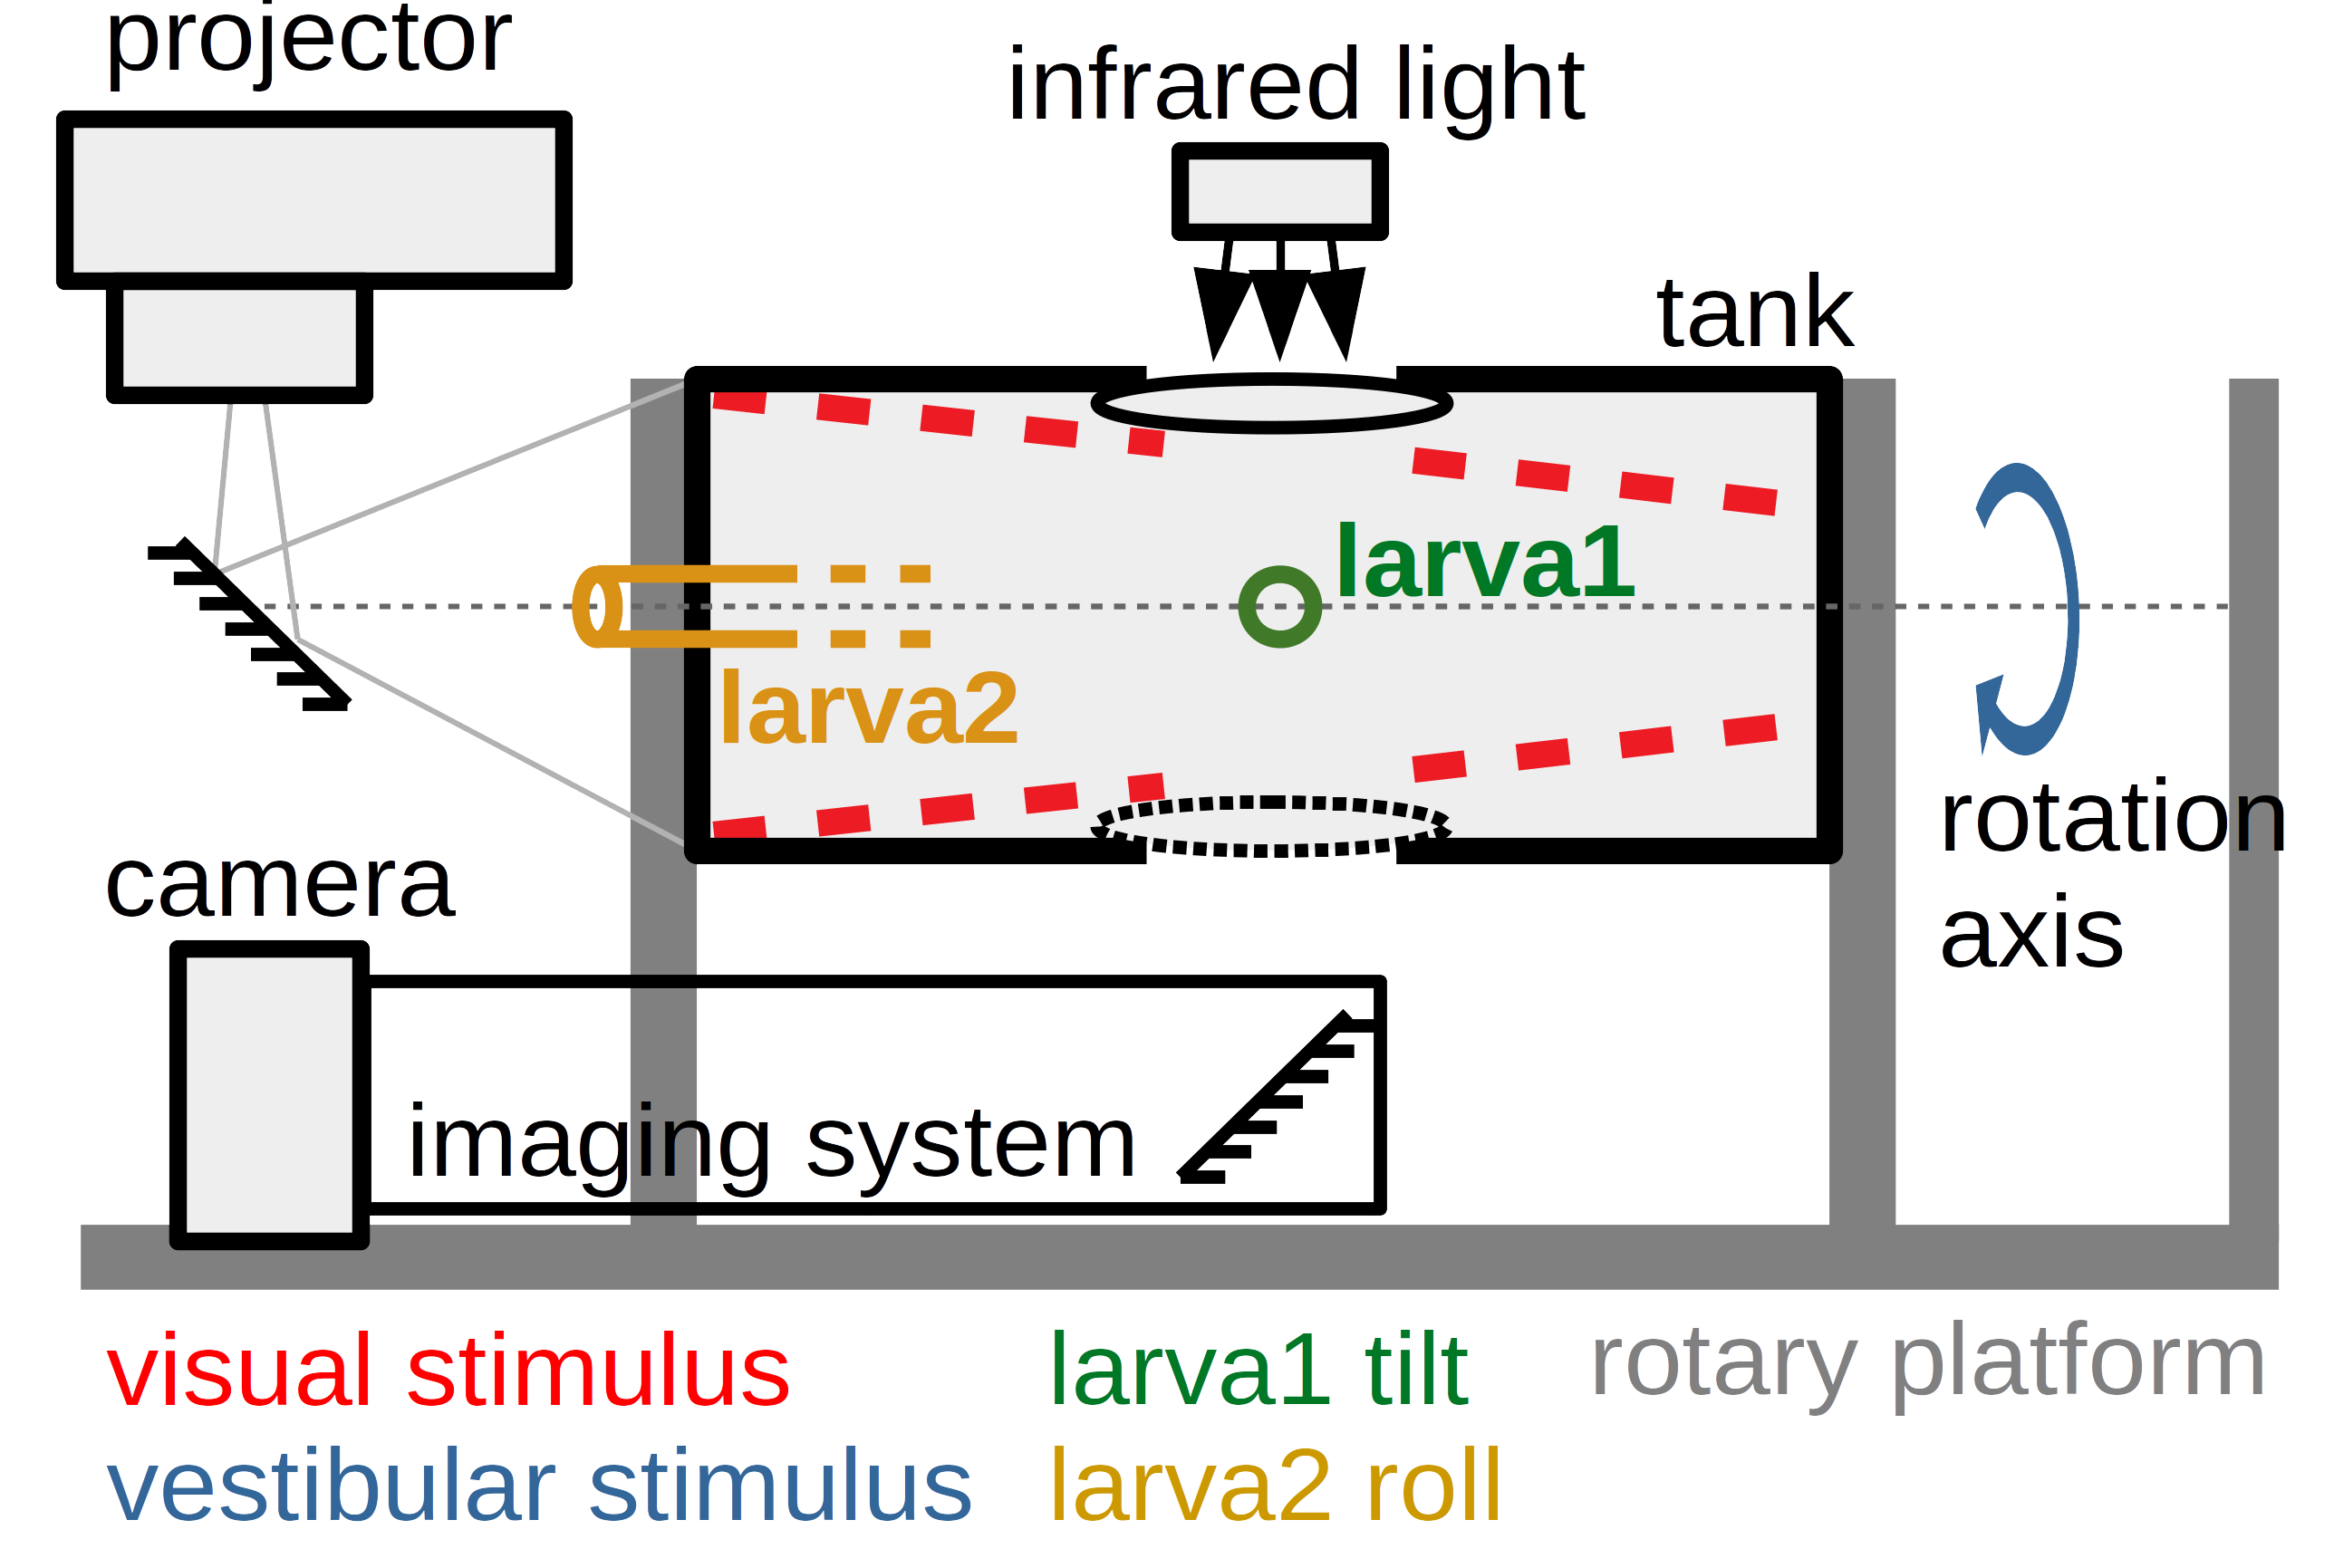
\includegraphics[width=0.8\textwidth]{./files/schema_manip.png}
\caption{Plateforme expérimentale permettant d'étudier le contrôle postural d'une larve de poisson zèbre pendant une boucle de rétroaction.}
\end{figure}

\subsubsection{Stimulation vestibulaire}
Le but de la cuve rotative est de soumettre le poisson à un stimulus vestibulaire contrôlé, et de pouvoir agir rapidement sur la commande (position angulaire, vitesse angulaire). Le moteur que j'ai utilisé pour entraîner la plateforme est le modèle DMAC17 de l'entreprise [midi-ingéniérie](http://www.midi-ingenierie.com/). Le modèle était assez ancien et ne disposait que d'une interface rudimentaire, j'ai donc du réimplémenter une commande série pour communiquer avec le microcontrôleur de la commande moteur. Finalement, la communication introduit une latence de quelques dizaines de millisecondes et impose un délai entre deux instructions. Cela semble cependant suffisant pour garantir une bonne impression de réalité virtuelle, puisque chez l'humain, les effets liés à la latence commencent à se faire sentir à partir de 75 ms \cite{waltemate_impact_2016}. Un problème que j'ai rencontré au début était les mouvements de l'eau dans la cuve. Le poisson y est très sensible via sa ligne latérale postérieure, ce qui faussait les expériences. En modifiant légèrement la cuve, j'ai pu maintenir l'eau de la cuve pratiquement immobile.

\subsubsection{Imagerie et analyse}
Pour détecter de manière fiable les mouvements de queue du poisson, j'ai mis au point un système d'imagerie adapté. Le système doit être léger et compact, afin de limiter le couple lors de la rotation de la plateforme et être insensible aux vibrations. Le poisson est éclairé par une lampe infrarouge à travers un diffuseur et une fenêtre située en haut de la cuve. En bas de la cuve, une autre fenêtre étanche laisse passer la lumière vers un miroir sur lequel pointe une caméra équipée d'un objectif grossissant et d'un filtre infrarouge. L'utilisation de la lumière infrarouge, invisible pour le poisson, permet de conserver la même qualité d'image quelque soit l'environnement visible pour le poisson. Les fenêtres sont les plus petites possible et situées dans l'extrémité du champ de vision du poisson afin de contrôler au mieux son environnement visuel. Le miroir permet de conserver la caméra et l'objectif proche de l'axe de rotation de la plateforme, pour limiter le bras de levier.
L'objectif du système d'imagerie est choisi pour que le poisson soit imagé sur un nombre réduit de pixels de la caméra. Ainsi, le transfert de donnée depuis la caméra vers l'ordinateur et le traitement de l'image sont rapides, ce qui permet de ne pas ralentir la rétroaction. Le traitement de l'image est simpliste mais fonctionnel. Il consiste à appliquer les fonctions suivantes :

- filtre de Sobel (fonction `edge` de Matlab, option `sobel`)
- dilatation (fonction `imdilate`)
- remplissage (fonction `imfill`)
- ouverture (fonction `bwareaopen`)
- ellipse équivalente (fonction `regionprops`, option `Orientation` )

Ce qui permet de trouver l'angle du poisson de manière reproductible d'une image sur l'autre, afin de détecter les mouvements de queue.

\begin{figure}
\centering
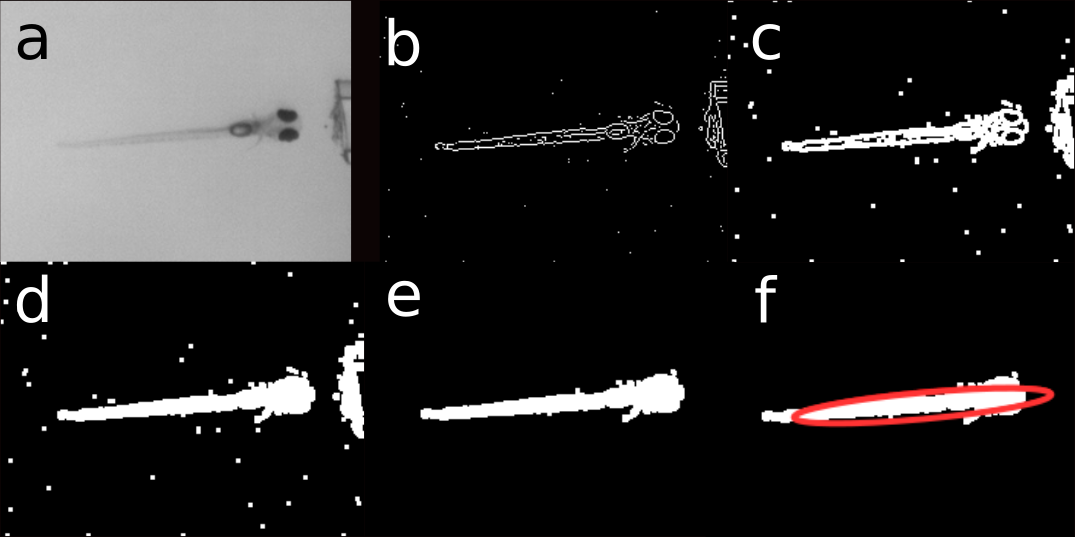
\includegraphics[width=0.8\textwidth]{./files/image_process.png}
\caption{Traitement d'image en cinq étapes pour obtenir l'angle du poisson. a) image originale sous éclairage infrarouge b) filtre de Sobel c) dilatation morphologique d) remplissage des contours e) ouverture morphologique f) ellipse équivalente via les moments d'ordre deux de l'image}
\end{figure}

% TODOVolker add figure with tail bend / struggle

\subsubsection{Stimulation visuelle}
Pour avoir un contrôle très souple sur l'environnement visuel du poisson du point de vue des couleurs, de la luminosité, et des formes, la solution idéale est un projecteur. Afin d'obtenir un bon contraste, les parois de la cuve sont coniques et blanches, réalisées dans un cylindre de PVC. Un cache évite d'éclairer directement le poisson pour ne pas perturber son environnement visuel. Les motifs sont réalisés à l'aide de \href{http://psychtoolbox.org/}{psychtoolbox}, une bibliothèque conçue pour l'affichage de stimulations visuelles. Pour conserver une fréquence d'affichage indépendant de la boucle de rétroaction et ainsi garantir un taux d'image par seconde constant d'expérience en expérience, j'ai séparé le processus de la boucle principale, avec laquelle il communique par le protocole TCP/IP.

\subsubsection{Insertion de la larve}
Pour immobiliser la larve de poisson zèbre, il est fréquent de la piéger dans un gel d'agarose à basse température de fusion concentré à 2\% aspiré par un capillaire en verre de diamètre intérieur 0.8 mm. La larve peut ainsi être insérée et maintenue par des trous de 1.4 mm, le diamètre extérieur du capillaire. Il en existe deux dans ma cuve : l'un sur l'axe de rotation pour étudier la réponse comportementale à une stimulation en roulis, l'autre perpendiculaire pour étudier la réponse à une stimulation en tangage. Afin d'observer les mouvements de la queue, je la libère en retirant la partie du bondin d'agarose qui l'entoure. 

\begin{figure}
\centering
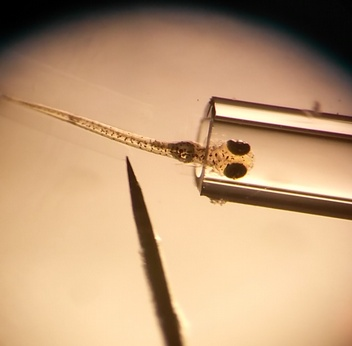
\includegraphics[width=0.8\textwidth]{./files/prepa_larve.png}
\caption{À l'aide d'un scalpel, un boudin d'agar est retiré de la queue d'une larve pour lui permettre de bouger. La larve est retenue par la tête et le corps, l'autre partie du boudin étant tenue par le capillaire en verre. }
\end{figure}

\subsection{Protocoles et résultats}

\subsubsection{Test par l'OMR}
Après avoir inséré un poisson dans la cuve, je le laisse reposer une à deux minutes pour lui permettre de s'adapter à son nouvel environnement. Je teste ensuite son réflexe optomoteur (OMR). Si le poisson ne réagit pas à cette stimulation visuelle, il est possible que sa vision ou sa motricité ne fonctionne pas, ou que son cerveau ne soit pas dans un état propice à l'étude de son système sensori-moteur. Pour tester l'OMR, je présente une alternance de bandes noires et blanches d'une taille apparente de trente degrés défilant à une vitesse apparente de vingt degrés par seconde, uniquement sur la partie basse de l'environnement visuel. Ce protocole est inspiré par celui présenté par Kris Severi \cite{severi_neural_2014}. J'ai réalisé ce test en boucle ouverte, c'est-à-dire sans rétroaction. Dans ce régime, le poisson présente un phénomène d'habituation si la stimulation dure trop longtemps, j'ai donc alterné des périodes de dix secondes de bandes fixes et dix secondes de bandes mobiles.

% This is the protocol also in the literature. If I remember correctly this is what Kris used in here paper. It would be good if you add references here

\begin{figure}
\centering
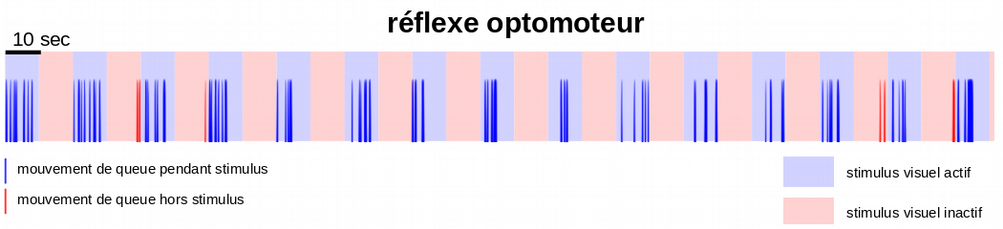
\includegraphics[width=0.8\textwidth]{./files/omr.png}
\caption{Expérience d'OMR en boucle ouverte. On voit que le poisson nage systématiquement en présence de stimulation visuelle (440 événements sur 150 secondes) et qu'il nage très rarement en absence de stimulation visuelle (22 événements sur 150 secondes).}
\label{FigOMRopenloop}
\end{figure}

Ces expériences sur le réflexe optomoteur montrent que le stimulus visuel projeté est suffisant pour étudier les réponses de la larve à son environnement visuel (Fig. \ref{FigOMRopenloop}).

\subsubsection{Rétroaction vestibulaire}
Pour mettre en place la boucle de rétroaction vestibulaire, je me suis inspiré de l'étude en nage libre de Ehrlich \emph{et al} \cite{ehrlich_control_2017}. J'ai choisi une vitesse de chute de 6°/s et une correction angulaire rapide de 10° lors d'un mouvement (en 100 ms environ). Ainsi, le poisson peut se maintenir à un angle fixe avec un mouvement toutes les 1.6 secondes. Si le poisson est immobile, son angle diminue jusqu'à l'angle limite que j'ai fixé à -60°. Ces expériences ont été réalisée dans le noir ou en éclairage uniforme, pour étudier la perception vestibulaire indépendamment de la perception visuelle.

\begin{figure}
\centering
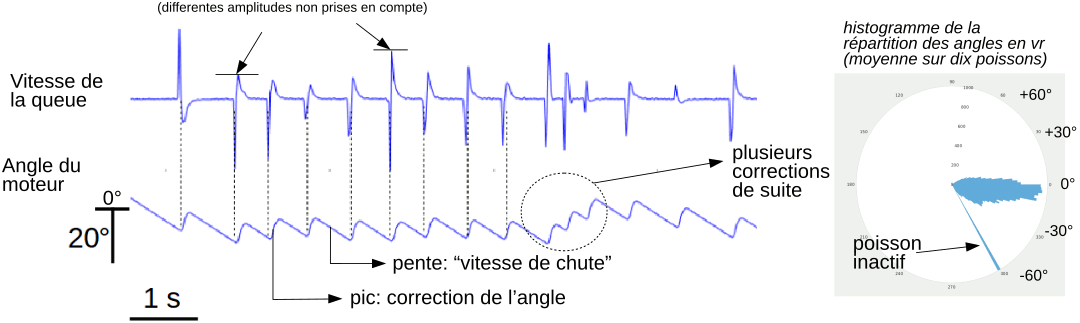
\includegraphics[width=0.8\textwidth]{./files/vestibular_feedback.svg.png}
\caption{Zoom sur un exemple de contrôle de posture dans une boucle de rétroaction virtuelle. Le poisson est soumis à un stimulus vestibulaire constant (pente constante) en l'absence de comportement. Lors d'un mouvement de nage, une rétroaction sur l'angle de la plateforme simule une correction d'angle du poisson.}
\end{figure}

Les paramètres de la boucle sont la vitesse de chute et l'angle de correction lors du mouvement. Pour répondre à une modifications de ces paramètres, le poisson doit adapter la fréquence de ses mouvements, car l'amplitude n'est pas prise en compte. Ainsi, à correction angulaire fixe, si la vitesse de chute augmente, comme dans l'expérience de la vessie natatoire remplie d'huile, le poisson doit augmenter la fréquence de ses mouvements. Au contraire, à vitesse de chute fixe, si la correction angulaire augmente, le poisson doit baisser la fréquence de ses mouvements. C'est effectivement ce que l'on constate dans les expériences, où une vitesse de chute de 2°/s, 4°/s et 6°/s avec une correction angulaire de 10° entraînent respectivement chez la larve une fréquence de mouvement de 0.2 Hz, 0.4 Hz, et 0.6 Hz en moyenne.

\begin{figure}
\centering
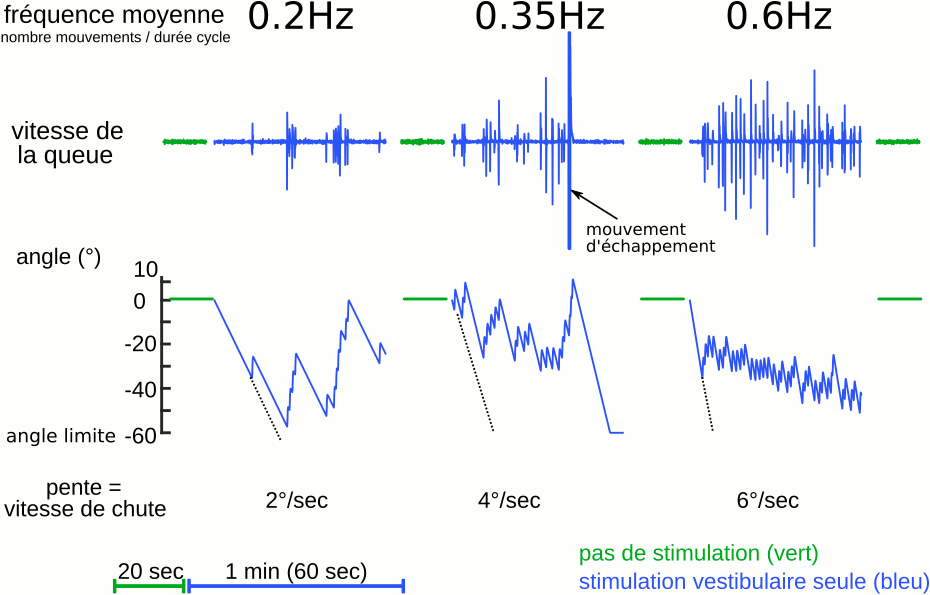
\includegraphics[width=0.8\textwidth]{./files/variation-vitesse.svg.png}
\caption{
Réponse d'une larve à une variation de la vitesse de chute. Trois cycles de une minute de stimulation vestibulaire sont séparés de pause de dix secondes. Le poisson se maintient autour d'un angle de -20° quelle que soit la vitesse de chute imposée, en adaptant la fréquence de ses mouvements.
\\
La fréquence moyenne du deuxième cycle est légèrement inférieure à sa valeur attendue (0.35 Hz au lieu de 0.4 Hz). Cela est du au fait que, suite à un mouvement d'échappement, le poisson est totalement inactif à la fin du cycle et stationne à -60°. Si l'on calcule la fréquence en ignorant les dix dernières secondes, la fréquence moyenne est bien de 0.4 Hz.
}
\end{figure}


La principale difficulté de ces expériences est le fait que le poisson peut devenir inactif et stationner à l'angle minimal autorisé par le système (-60°). C'est pour cette raison que la durée choisie pour les cycles est relativement courte (60 secondes). À la fin d'un cycle, le poisson est ramené à l'angle de référence (0°). Cela évite que le poisson reste trop longtemps inactif, état dans lequel il est impossible d'étudier le contrôle postural. Pour obtenir des fréquences représentatives, il faut donc les calculer uniquement sur les périodes d'activité.

On observe ce même comportement sur des larves dans une boîte de pétri : de temps en temps elles cessent toute activité et reposent sur le fond de la boîte. La boucle de rétroaction du contrôle postural est alors en pause. Dans le cas d'un larve prisonnière d'un boudin d'agarose, les périodes d'inactivité font souvent suite à un mouvement d'échappement (*struggle*), pendant lequel la larve tente de s'échapper en se tortillant sur elle même avec des mouvements de très grande amplitude.

\subsubsection{Protocole multimodal}
L'intérêt de l'environnement virtuel est qu'il est possible de contrôler à la fois la stimulation vestibulaire et la stimulation visuelle. Après avoir étudié le contrôle postural dans le noir, j'y ai ajouté une composante visuelle. L'objectif est de comparer la réponse en cas de stimulation multimodale par rapport aux réponses en présence des deux stimuli séparément.

\begin{figure}
\centering
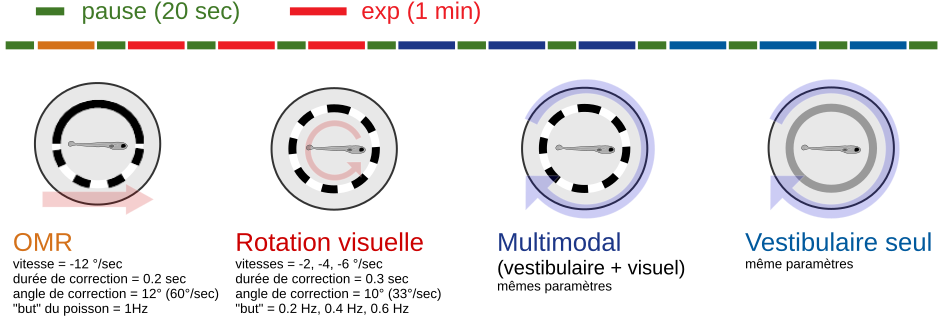
\includegraphics[width=0.8\textwidth]{./files/protocole_multimodal.svg.png}
\caption{
Exemple de protocole multimodal, faisant intervenir à la fois une stimulation vestibulaire et une stimulation visuelle. Des cycles d'une minute sont séparés par des pauses de vingt secondes.
}
\end{figure}

Le protocole commence par un cycle d'OMR qui permet d'évaluer le niveau d'activité du poisson. S'il ne répond pas à cette stimulation, l'expérience est interrompue pour passer au poisson suivant, ce qui évite d'observer pendant un quart d'heure une larve immobile. Ensuite vient une phase de stimulation purement visuelle avec rotation de l'ensemble de l'environnement, tout autour du poisson. Pendant cette phase, l'information visuelle indique au poisson qu'il tourne, ce qui est en conflit avec l'information vestibulaire. La partie inférieure du champ visuel est similaire à une stimulation d'OMR, mais la partie supérieure diffère. Il est de toute façon difficile de différencier les deux. Ensuite, en conservant le motif de la phase visuelle en position fixe dans le référentiel du laboratoire, la cuve tourne avec le poisson pour stimuler le système vestibulaire, utile au contrôle postural. Pendant cette phase, les deux modalités sensorielles sont cohérentes. Elles indiquent toutes les deux au poisson qu'il est en train de tourner. Ensuite, le motif est remplacé par un éclairage uniforme d'intensité moyenne identique. Cela permet de conserver une luminosité ambiante dans la cuve identique au cycle précédent. Cette phase est celle exposée précédemment, dans la partie sur la rétroaction vestibulaire. Chaque phase est séparée en trois sous-phases, avec trois vitesses de stimulus différentes (2, 4, et 6 degrés par seconde), pour étudier l'adaptation au conditions virtuelles.

\begin{figure}
\centering
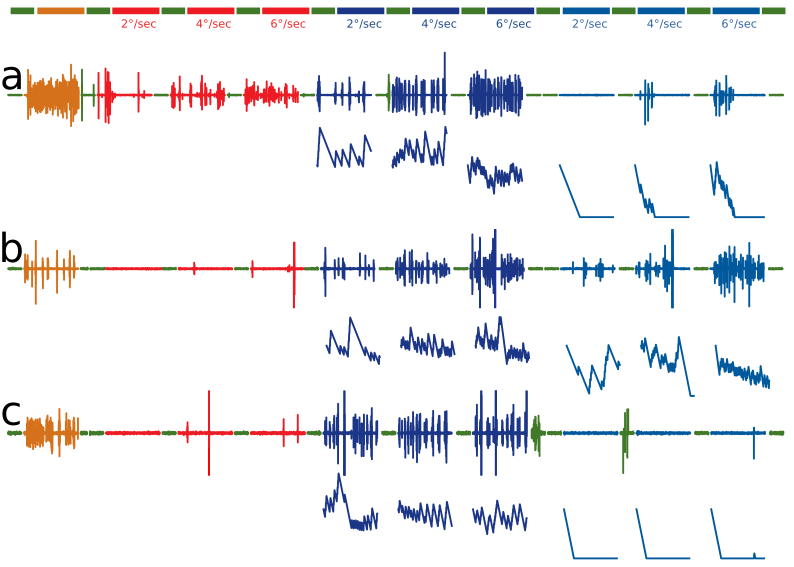
\includegraphics[width=0.8\textwidth]{./files/raw_data.svg.png}
\caption{
On voit ici le protocole appliqué sur trois poisson différents. Dans tous les cas, la réponse optomotrice fonctionne, mais on voit des différences au niveau des autres stimuli. Le poisson `a` répond bien à la stimulation visuelle, mais quasiment pas à la stimulation vestibulaire, le poisson `b`, au contraire, ne répond pas à la stimulation visuelle (bien qu'il réponde à l'OMR), mais répond à la stimulation vestibulaire pure. Le poisson `c` ne répond ni à la stimulation visuelle pure, ni à la stimulation visuelle pure, mais répond comme les deux autres pendant le cycle multimodal.
\\
Ces comportements spécifiques à un poisson sont reproductibles. Le protocole a été répété cinq fois sur le poisson `a` avec toujours la même réponse.
}
\end{figure}

La réponse des larves à ce protocole est très variable. De nombreuses données sont inutilisables à cause d'une larve immobile après un mouvement d'échappement, mais dans les données restantes, certains poissons montrent une bonne réponse principalement au stimulus vestibulaire seul, d'autres au stimulus visuel seul, alors que la plupart répondent bien pendant le cycle multimodal. Il semble donc qu'en fonction des poissons l'importance relative des différentes modalités sensorielles dans le contrôle postural soit variable. Pour certains poissons, cependant, la présence simultanée des deux modalités sensorielles semble nécessaire au contrôle postural. Cela peut être interprété de la manière suivante.

Pendant les phases unimodales visuelles, les sensations visuelle et vestibulaire sont en conflit, ce qui peut réduire et même supprimer la réponse motrice, la force de cet effet variant d'un poisson à l'autre. Dans les phases unimodales vestibulaires, le poisson ne reçoit aucune information visuelle sur sa position et la réponse comportementale peut être affaiblie par un manque de fiabilité de l'information vestibulaire. Au contraire, pendant les phases de stimulus multimodal cohérent, on remarque une réponse comportementale forte, augmentée par l'intégration multisensorielle.

% During the unimodal visual phases the visual and vestibular sensations are in conflict reducing or suppressing the motor response. The strength of this effect varies between fish. In the unimodal vestibular case where the fish does not receive and visual information about its body rotation the behavioral response might be weak due to the unrelieability of the vestibular stimulus. However, in the coherent multimodal case we see a strong multisensory enhanced behaviorial response 

\subsubsection{Interprétation}
Malgré ces comportement individuels variables, on peut analyser globalement la réponse des larves. La métrique utilisée est la fréquence moyenne des mouvements, calculée comme le rapport entre la quantité de mouvements de nage et la durée du cycle. Cette métrique inclut les périodes d'inactivité qui suivent un mouvement d'échappement, ce qui fausse légèrement la valeur, comme montré dans l'exemple de rétroaction vestibulaire. On observe néanmoins deux phénomènes : le poisson est capable de moduler son activité en fonction de la force du stimulus, et le poisson a une réponse plus forte en présence de deux stimuli cohérents .

\begin{figure}
\centering
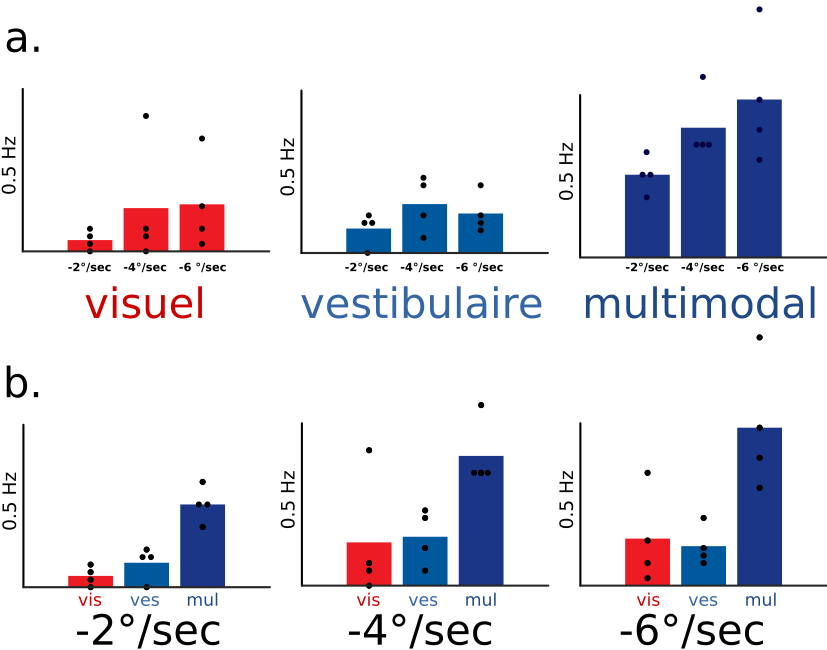
\includegraphics[width=0.8\textwidth]{./files/stats.svg.png}
\caption{
Analyse réalisée sur dix poissons différents parmi trente soumis au protocole. Les valeurs à zéro (poisson entièrement inactif) sont retirées, et il reste donc environ quatre points par moyenne.
\\
a. Pour chaque cycle, on observe une adaptation du poisson à la force du stimulus. Le poisson est capable d'adapter sa fréquence de nage pour se stabiliser par rapport à une information visuelle ou vestiblaire.
\\
b. Pour chaque vitesse de stimulus, on observe une réponse moyenne différente en fonction du type de stimulus. Alors que le stimulus vestibulaire et visuel pur sont d'efficacité comparable, la présence simultanée des deux modalité sensorielles entraîne globalement un meilleure réponse chez les larves.
}
\end{figure}

% TODOVolker Perspective and interpretation of the results is still to develop. 

On a montré qu'il était possible de reproduire la boucle de rétroaction sensorimotrice du contrôle postural dans un environnement virtuel. Une des principales limitations est l'immobilisation de la larve, qui provoque des mouvements violents d'échappement suite auxquels la larve est inactive pendant une longue durée. Cela réduit considérablement la quantité de données exploitables (environ 90\% des expériences sont en partie ou totalement inutilisables), les données présentées ici sont donc statistiquement faibles.

Ces résultats montrent qu'un réflexe \emph{a priori} vestibulaire comme le contrôle postural est en réalité largement altéré par d'autres modalités sensorielles comme le système visuel. On peut supposer que la sensation tactile, qui permet au poisson de sentir les écoulemements de fluide, joue également un rôle (que je n'ai pas testé). La reproduction de la boucle sensorimotrice dans un environnement en réalité virtuelle ouvre la possibilité d'étudier les mécanismes cérébraux qui en sont à l'origine. Pour comprendre en profondeur ces mécanismes, il est nécessaire de simuler un environnement sensoriel riche  

Une piste d'évolution importante serait de limiter ces comportements d'échappement. 
% escape/startle/struggle
%TODOcite
% - Escape Behavior Elicited by Single, Channelrhodopsin-2-Evoked Spikes in Zebrafish Somatosensory Neurons
% - Imaging the Functional Organization of Zebrafish Hindbrain Segments during Escape Behaviors
% - Evidence for a Widespread Brain Stem Escape Network in Larval Zebrafish
% - Imaging escape and avoidance behavior in zebrafish larvae
Ceux-ci diminuent largement l'échantillon statistique en inhibant l'activité du poisson pendant de longues périodes, ce qui rend l'analyse difficile. Cette amélioration pourrait être obtenue en modifiant la manière dont le poisson est retenu immobile et en ajustant les paramètres de rétroaction en fonction des poissons. 

\subsection{Conclusion}

% TODOVolker Perspective and interpretation of the results is still to develop. 
\chapter{Imagerie fonctionnelle sous stimulation vestibulaire}\label{chapIII}

% TODO VolkerComment
% You have to extent significantly the first paragraph and link it to the previous chapter. For the following subsections you have to seperated Geoffrey's development from your developments. When you started your PhD the one-photon system was already developed by Geoffrey. You have to review this development in all details to prepare the chapter where you present the two-photon RLS and your developments. Especially, you have to talk about the fiber delivery of the laser onto the rotating platform. Do not mix this presentation with any developments that yo did later for the 2PRLS. Your contribution comes when you talk about the challenges posed by treating the recorded large data sets and the necessity of the development of an analysis pipeline. Introduce well the analysis challenges and the requirement that a good analysis pipeline should fulfill. Then you write an entire chapter to detail your easyRLS development. This routine became the bases for the data analysis in the paper and is our work horse in the group until today. This development gave you a first publication.


\section{Microscope rotatif}

% transition
Dans le chapitre précédent, je montre comment tester le comportement d'intégration visuo-vestibulaire dans un environnement en réalité virtuelle. L'objectif est d'observer l'activité du cerveau lors d'un tel comportement. Pour cela, il faut un système capable de réaliser l'enregistrement neuronal en même temps que la stimulation des systèmes vestibulaire et visuel. Cet objectif présente plusieurs difficultés : exciter le système vestibulaire tout en gardant le poisson fixe par rapport à l'objectif de microscope et contrôler son environnement visuel en dépit du laser d'excitation de fluorescence. Dans ce chapitre, je m'intéresse à la partie vestibulaire.

Pour stimuler le système vestibulaire tout en gardant le poisson fixe par rapport à l'objectif, une option est d'agir directement sur l'organe vestibulaire sans bouger la larve. C'est la solution adoptée par Favre Bulle \emph{et al} dans un article publié en 2017 \cite{favre-bulle_optical_2017}. Les auteurs ont utilisé des pinces optiques pour stimuler directement les otolithes. Cette solution est limitée, car il n'est pas possible de calibrer la force appliquée, la concentration du laser produit un échauffement qui limite la durée maximale de la stimulation, et la gamme de force applicable est restreinte.

Au Laboratoire Jean Perrin, Geoffrey Migault et Volker Bormuth se sont tourné vers une autre option : tourner réellement le poisson pour que la gravité bouge ses otolithes.
% Papi Jean est mort. Je m'arrête un moment.
Cette deuxième solution est plus performante, car elle reproduit réellement la stimulation vestibulaire sans les limitations dues aux pinces optiques, mais elle nécessite des développements techniques avancés pour être appliquée sous microscope. En effet, pour conserver le microscope fixe par rapport à un poisson mobile, il faut construire un microscope rotatif, tout en gardant les conditions de stabilité nécessaires à l'imagerie. Un microscope à feuille de lumière rotatif capable de mesurer l'activité du cerveau pendant une stimulation vestibulaire réelle a donc été développé \cite{migault_whole-brain_2018}.

\subsection{Description du montage}

\subsubsection{Unité d'illumination}

Un microscope à feuille de lumière par balayage est généralement constitué de deux bras optiques formant un télescope de manière à placer le miroir rotatif galvanométrique de balayage dans le plan congugué de l'échantillon. Ainsi, son mouvement de rotation est transformé en une pure translation du faisceau au niveau de l'échantillon. Ce montage est volumineux et inadapté à un microscope rotatif. Il a donc fallu le miniaturiser et garantir sa stabilité. Les télescopes ont été remplacés par des objectifs de microscope. Le plan de Fourier n'étant pas accessible à cause de la distance frontale arrière, le miroir galvanométrique est légèrement hors du plan conjugué, ce qui introduit une rotation du faisceau dans l'échantillon en plus de la translation. Cette rotation reste cependant faible (<0.4°), et compatible avec une feuille de lumière par balayage.  
L'unité d'illumination est composée d'un connecteur de fibre monté sur un positionneur piézoélectrique et de deux objectifs en montage confocal de part et d'autre d'un miroir galvanométrique. 

\begin{figure}
\centering
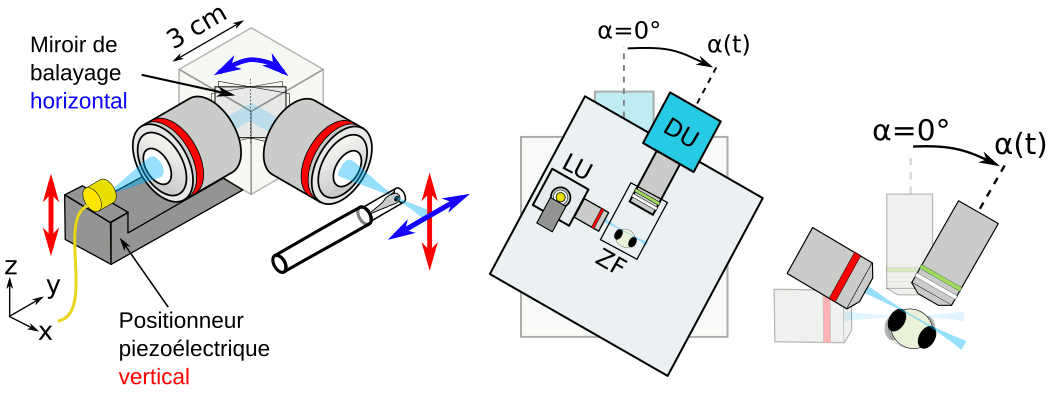
\includegraphics[width=0.8\textwidth]{./files/miniature_light-sheet.svg.png}
\caption{Schéma extrait de l'article \cite{migault_whole-brain_2018}. Le module miniature peut être monté sur un microscope rotatif. Le poisson est positionné dans l'axe de rotation, et tourné en roulis. L'illumination vient par le côté.
}
\end{figure}

\subsubsection{Unité de détection}

L'enjeu pour une unité de détection rapide est de permettre l'enregistrement avec une durée d'exposition la plus courte possible tout en maintenant un rapport signal à bruit suffisant. Pour collecter beaucoup de lumière, il faut une grande ouverture numérique, et donc une distance de travail faible. Cependant, pour une imagerie à champ large, il faut un grandissement faible. La solution retenue est un objectif Olympus d'ouverture numérique 1 et de grandissement x20. Le grandissement est donné pour une lentille de tube de 180 mm, mais une lentille de tube de 150 mm a été utilisée, ce qui donne donc un grandissement de x16.667. Un pixel de la caméra mesure 6.5 µm, ce qui donne un pixel objet de 0.39 µm. Le capteur CMOS est un carré de 2048 pixels de côté, ce qui donne un champ objet de 0.8 mm. Le champ objet correspond à la longueur du cerveau, mais le pixel objet est très petit par rapport à un neurone. Pour limiter la quantité de données à enregistrer et augmenter le rapport signal à bruit, on peut combiner par les pixels de la caméra, opération appellée \emph{binning}. Cela donne un pixel objet de 0.78 µm.

\begin{figure}
\centering
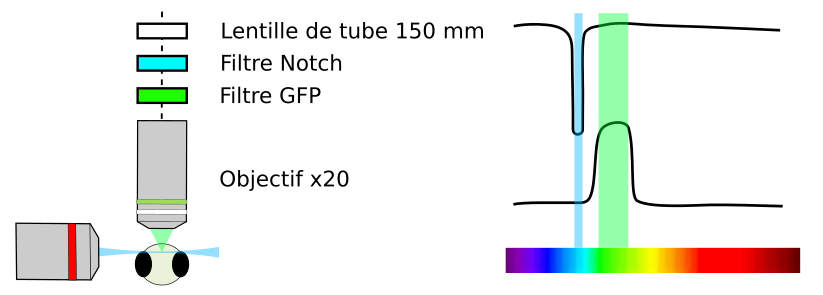
\includegraphics[width=0.8\textwidth]{./files/detection_unit.svg.png}
\caption{Schéma du filtrage spectral dans le bras de détection. Le filtre notch (\emph{encoche}) est très étroit et rejette la longueur d'onde du laser (488 nm). Le filtre GFP et plus large et transmet seulement une bande autour de la fréquence de la GFP (525 nm).}
% 1e-5 à 488 nm pour GFP
% 1e-6 à 488 nm pour Notch
\end{figure}

% OK VolkerComment
% Originally, we did the experiments only with the notch filter. All photons emitted by the fluorophore were then collected which maximizes the signal. The GFP filter helps to block some additionally excited autofluorescence in the tissue. With the GFP filter the notch filter is not really anymore necessary. You can keep your figure but show the real GFP filter transmission spectrum in this case !

Pour obtenir un bon rapport signal à bruit, il faut réduire la lumière parasite. Une source puissante est le laser d'illumination, elle peut être bloquée spécifiquement avec un filtre coup bande très étroit à sa longueur d'onde. Un filtre GFP (passe-bande à la longueur d'onde de la GFP) permet de filtrer davantage l'autofluorescence des tissus. Après ce filtrage, les bruits restants sont le bruit de photon et le bruit numérique. Le bruit numérique pourrait être réduit avec un système de refroidissement prévu sur la caméra, mais celui-ci est trop encombrant pour le microscope rotatif, et a donc été retiré. Le bruit de photon ne peut être réduit qu'avec des meilleures sondes calciques ou en exposant plus longtemps, mais il est négligeable devant le bruit numérique d'une caméra non refroidie. Le bruit numérique présente une structure liée à la constitution interne du capteur et qui fait apparaître des raies de pixel et la ligne médiale de l'obturateur déroulant.

% OK VolkerComment
% No! We do not filter out light from light sources in the room! The systems are shielded such that this light does not enter the detection path . The GFP filter filters additional excited autofluorescence.

% L'unité de détection est composée d'un objectif à immersion (le poisson est dans l'eau) monté sur un positionneur piézoélectrique, d'une lentille de tube, d'un filtre coupe-bande, d'un filtre GFP, et d'une caméra.

\subsubsection{Stabilité mécanique}

Le tout pèse environ 2 kg (?) et tient sur une plaque de 50 cm de côté fixée à un moteur à grand couple et grande précision. Le moteur dispose d'un grand rotor permettant une large zone de fixation qui minimise les déformations mécaniques de la plaque qui soutient le microscope. Nous avons caractérisé précisément l'instabilité liée à la rotation du microscope à l'aide de billes micrométriques fluorescentes.

\begin{figure}
\centering
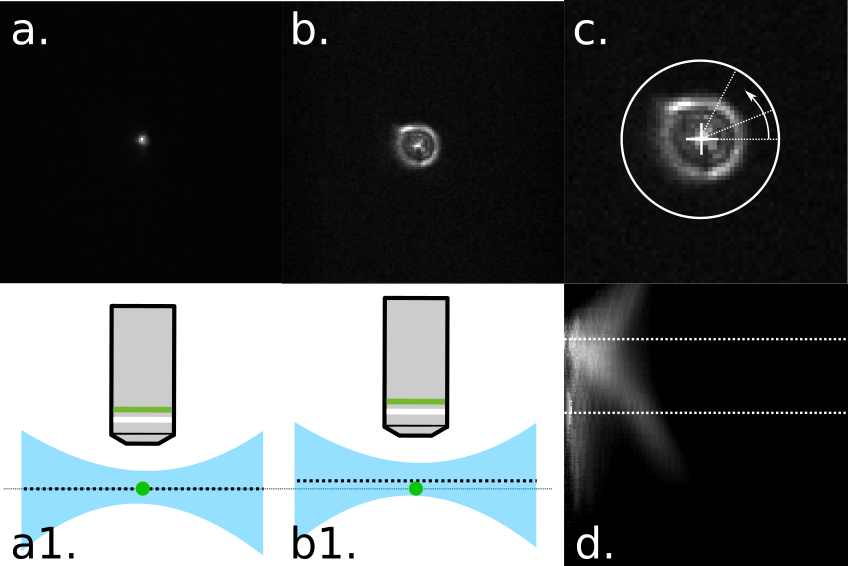
\includegraphics[width=0.8\textwidth]{./files/bead_position.svg.png}
\caption{Schéma des étapes pour estimer avec précision la position d'une bille fluorescente.\\
a. Image d'une bille dans le plan focal de l'objectif (a1)\\
b. Image d'une bille hors du plan focal de l'objectif (a2)\\
c. Établissement du profil radial par moyennage autour du centre de gravité de l'image\\
d. Profil cylindrique de la figure de diffraction constitué du profil radial pour plusieurs positions de l'objectif espacées de 20 nm. Les traits pointillés correspondent aux plans (a) et (b). La corrélation verticale du profil cylindrique pour plusieurs positions du microscope donne avec précision le déplacement de la bille.
\label{FIGbeadstability}}
\end{figure}

Une bille fluorescente de 1 µm est éclairée transversalement par le laser d'excitation, qui coïncide avec le plan focal de l'objectif de détection. Elle est imagée pour plusieurs positions hors focus de l'objectif, ce qui fait apparaître des franges d'interférence. Un profil cylindrique de ces franges est réalisé pour plusieurs positions du microscope et à plusieurs intervalles de temps ce qui permet de mettre en évidence le déplacement latéral et vertical de la bille au cours du temps et en fonction de la position du microscope. Cette technique a l'avantage d'être précise (de l'ordre de 100 nm) et robuste aux variations liées au photoblanchiment. Elle a permis de montrer que lors de la rotation du microscope, le déplacement reste inférieur à 500 nm dans la direction verticale et 2 µm dans la direction latérale (cette dernière peut être corrigée lors de l'analyse comme on le voit plus tard).

\subsection{Nappe laser par balayage}

\subsubsection{Ouverture numérique optimale}

Le volume d'un cerveau de larve de poisson zèbre mesure 400 µm de largeur × 800 µm de longueur × 300 µm de hauteur et est situé sur le dessus de la larve. Afin de minimiser l'épaisseur de tissus traversée, on place donc l'objectif de détection sur la partie supérieure. Le laser peut donc être placé sur le côté. Les yeux sont très pigmentés et la lumière ne passe pas à travers, ce qui crée une zone d'ombre entre les yeux. Certains laboratoires qui sont intéressés par ces régions appartenant au télencéphale et au diencéphale peuvent donc ajouter un deuxième laser à l'avant pour éclairer cette région.

Pour produire un faisceau laser le plus fin possible sur une longueur de 400 µm, il faut minimiser la largeur après 200 µm de propagation avec comme variable le waist $w_0$ placé au milieu de l'échantillon :

$$
w(z) = w_0 \, \sqrt{ 1+ {\left( \frac{z}{z_\mathrm{R}} \right)}^2 } \qquad z_\mathrm{R} = \frac{n \pi w_0^2 }{\lambda}
$$

\begin{figure}
\centering
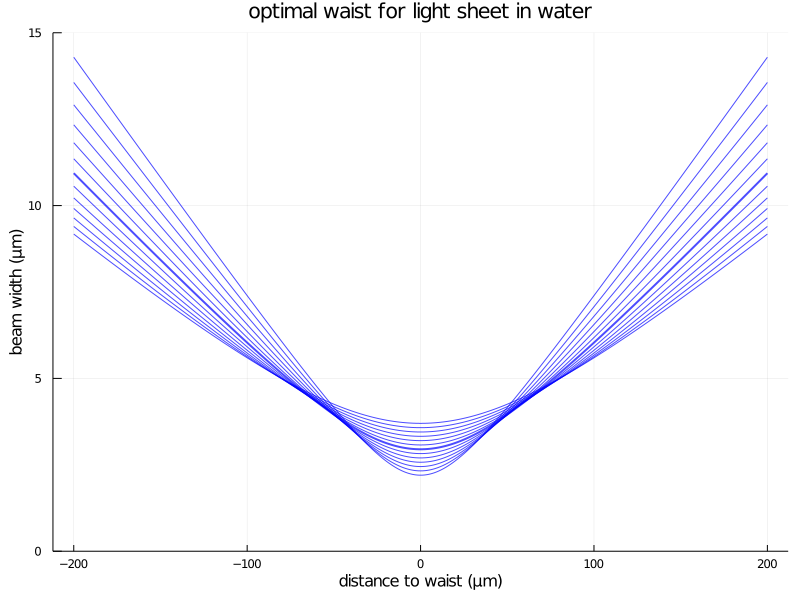
\includegraphics[width=0.8\textwidth]{./files/possible-waist_1P.png}
\caption{On voit ici la demie largeur du profil gaussien à 488 nm dans l'eau pour différentes valeurs du waist. Le trait en pointillé montre le rayon d'un neurone. On cherche à minimiser l'épaisseur du faisceau entre -100 µm à 100 µm. Le trait épais marque la position optimale pour ce critère (les autres profils sont tous plus larges à 100 µm du centre). L'ouverture numérique associée vaut $ \mathrm{NA} = n\sin(\lambda/\pi n w_0) $.}
\end{figure}

% OK VolkerComment
% Indicate the NA used for the different curves.

Un waist trop petit est trop divergeant, et donc trop large sur les bords, mais un waist trop large limite la résolution. Il faut donc trouver un optimum. La taille d'un neurone étant de 8 µm environ, des valeurs inférieures sont souhaitables.

Une valeur de waist possible pour un échantillon de 400 µm est de 3 µm à 488 nm et de 5 µm à 915 nm. Pour ces valeurs, la largeur du faisceau à 488 nm vaut 3 µm au centre et 10 µm sur les bords du cerveau. À 915 nm c'est 5 µm au centre et 14 µm sur les bords, mais il faut aussi prendre en compte l'effet deux photons. En pratique, la plupart des neurones sont situés entre -150 µm et +150 µm, la largeur du faisceau aux extrémités n'est donc pas critique.

\subsubsection{Balayage horizontal et vertical}

Pour effectuer le balayage, on déplace le faisceau horizontalement. Pour que l'intensité soit homogène sur une image, il faut adopter une vitesse de déplacement constante. Il est alors possible de faire un aller simple ou des allers-retours en nombre entier pendant le temps d'exposition. Pour obtenir une image volumétrique, il suffit de répéter l'opération pour plusieurs couches, en changeant le plan focal de l'objectif de détection et la position vertical de la nappe. Procéder de cette manière couche après couche force à attendre entre deux couches pour laisser le temps aux éléments mécaniques de se positionner, ce qui prend un temps (environ 10 ms) non négligeable pour des durées d'exposition courtes. Il est également possible de bouger les éléments mécaniques de manière continue en balayant en aller simple. Les couches sont donc légèrement obliques, mais on gagne considérablement en fréquence d'acquisition. Cela est possible grâce au mode \emph{synchronous readout} de la caméra qui permet de lire les valeurs d'une ligne de pixels tout en exposant une autre.


\begin{figure}
\centering
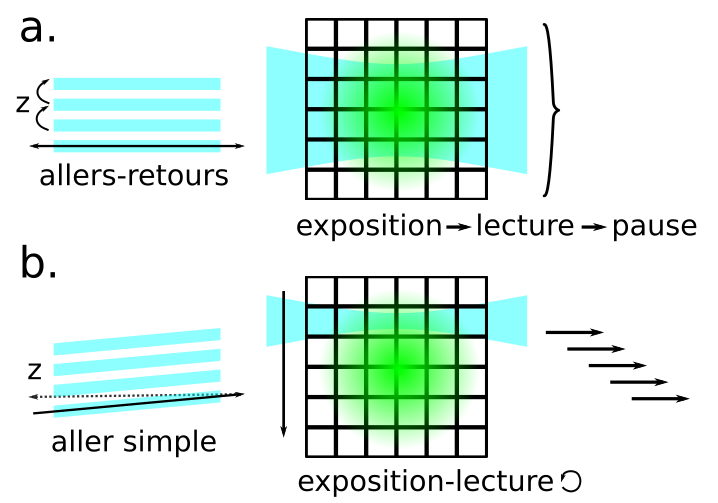
\includegraphics[width=0.6\textwidth]{./files/schema_balayage.svg.png}
\caption{Différents modes de balayage et de lecture du capteur CMOS. Les couches z successives sont représentées à gauche, le capteur (dans le plan xy) est représenté à droite.\\
a. Balayage par allers-retours lors de l'exposition de tous les pixels, puis lecture de tous les pixels et déplacement à la couche suivante. Le déplacement étant lent, une pause est nécessaire. Pas d'exposition pendant la pause\\
b. Balayage par aller simple lors de l'exposition, lecture successives des rangées de pixels et ré-exposition immédiate. Le déplacement vertical est continu à vitesse constante, les couches en z sont légèrement obliques. Le cycle exposition-lecture est décalé dans le temps pour chaque rangée de pixels.}
\end{figure}
% Add a figure that shows the different scan protocols and that explains the camera readout

Pour un temps d'exposition par couche de 10 ms en mode d'acquisition continu, on peut par exemple réaliser un scan du cerveau à 2,5 Hz en 30 couches espacées de 8µm. Cela permet d'imager la majeure partie du cerveau du poisson. Les couches les plus profondes sont moins nettes, car le signal traverse plus de tissus avant d'atteindre l'objectif, et la zone située entre les yeux reste dans l'ombre si on n'utilise qu'un laser. Mais chaque neurone visible est imagé à une fréquence de 2.5 Hz.

% \subsubsection{Ordres de grandeur}
% -> Partie microscope





% \subsection{Caractérisation}


\section{Analyse des données}

L'analyse des données produites par le microscope est en enjeu en lui-même. En effet, avec des images de 1024$\times$600 pixels, 20 couches et 25 minutes d'enregistrement à 2 volumes par seconde (3000 pas de temps), on obtient 60000 images. Pour des pixels stockés sur 16 bits, cela donne près de 60 Go de données brutes. Dans ce chapitre, je m'intéresse aux stratégies pour traiter ces données. Les chiffres donnés ci-dessus sont ceux utilisés pour les calculs en ordre de grandeur par la suite.

\subsection{Logiciels existants}

\subsubsection{Fiji}

De nombreux laboratoires de biologie réalisent leur analyse d'image avec Fiji (une distribution du logiciel ImageJ). Cet outil générique offre en effet une bonne interface pour visualiser les données tout en y appliquant des transformations élémentaires, mais montre rapidement ses limites en termes de vitesse, d'automatisation, et de robustesse. Les différents laboratoires travaillant en imagerie neuronale se sont donc tournés vers des logiciels spécialisés.

\subsubsection{Suite2P}

Les laboratoires réalisant de l'imagerie deux photons sur le cerveau de rongeur ont des données de petit volume, mais nécessitant des algorithmes sophistiqués avant d'être exploitables. Le logiciel \href{https://www.suite2p.org/}{suite2p} \cite{pachitariu_suite2p_2016}, doté d'une interface graphique intuitive expose une routine puissante pour la correction de mouvement et la détection de cellules par leur activité. Quelques essais sur nos jeux de données ont montré que le logiciel était fonctionnel mais excessivement lent, ce qui rend l'analyse systématique impossible.

\subsubsection{CaImAn}

Plusieurs laboratoires travaillant en microscopie à feuille de lumière analysent leurs données à l'aide de \href{https://github.com/flatironinstitute/CaImAn}{CaImAn} (pour \emph{Calcium Image Analysis}) \cite{giovannucci_caiman_2019}. Ce programme est décliné en deux versions, la version \emph{online} pour l'analyse de données en temps réel sur une expérience en cours, et la version \emph{batch} pour l'analyse de données \emph{a posteriori}. La première nécessite des machines très puissantes pour atteindre le taux d'images par secondes requis alors que la seconde peut être exécutée sur des machines modestes. Le logiciel a été publié en 2019, je l'ai essayé sur nos jeux de données avec des résultats satisfaisants en termes de qualité, quoiqu'un peu lents.

\subsection{Solution utilisée pour l'analyse de nos données}

% OK VolkerComment
% You have to describe your development of easyRLS a routine in form of a collection of functions that allows in a modular manner to analyze the whole-brain data. Go more in detail.

Aucun logiciel adapté à nos données n'étant disponible à l'époque, nous avons développé nos propres méthodes adaptées à l'imagerie sur plateforme rotative. Les spécifications étant très mouvantes, nous avons adopté une structure modulaire dans laquelle une collection de fonctions peuvent être appliquées optionnellement dans un ordre adapté à chaque jeu de données. Je décris ici les étapes principales de l'analyse, les enjeux techniques, et les pistes d'amélioration.

\subsubsection{Étapes principales de l'analyse de données}

\paragraph{Espace de référence}

Dans la suite de cette section, j'appellerai de manière équivalente (x,y,z,t) les coordonnées d'un point et les axes dans le repère du poisson. Ces coordonnées sont données dans l'espace de référence RAST (\emph{Right Anterior Superior Time}), c'est-à-dire que l'axe x est orienté vers la droite de la larve, l'axe y vers l'avant, l'axe z vers le haut, et le temps dans le sens naturel.

\begin{figure}
\centering
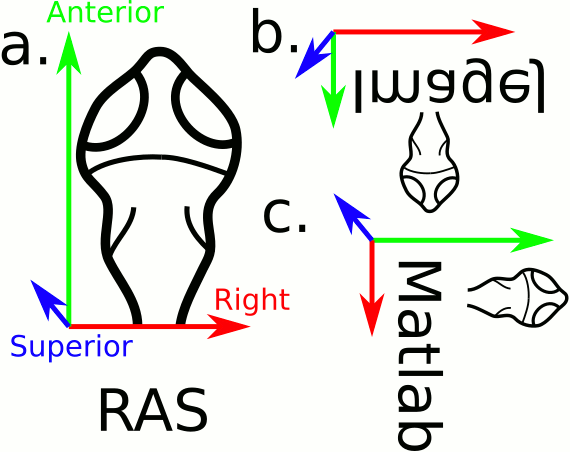
\includegraphics[width=0.6\textwidth]{./files/RAST.svg.png}
\caption{Illustration de la convention d'orientation RAS (a.) et comparaison avec les systèmes de coordonnées naturels de ImageJ (b. coordonnées des pixels d'un écran) et Matlab (c. coordonnées des éléments d'une matrice).}
\end{figure}

% OK VolkerComment
% Add a figure illustrating the RAST definition and add your wiki page with the corresponding figures about the different coordinate systems used in Matlab, Fiji, cmtk

\paragraph{Alignement temporel}

% OK VolkerComment
% Start introducing the problem. We have two main problems. Slow thermal drift and fast stimulus induced movements. In addition we have to scope with tissue deformation but normally we discard these runs. Then discuss the different approaches that you developed. Autocorrelation with the first image, autocorrelation with an average image, treatment of all layers independently, estimating the drift per stack based on one layer with good contrast or selecting high contrast landmarks to calculated the drift. Discuss that you developed different approaches: 1. Estimating the fast and slow movements together, 2. Estimating and correcting slow and fast drift sequentially. 3. Correcting the sinusoïdal stimulus induced fast component by hand by applying a sinusoïdal drift correction with user defined amplitude and phase. Make a figure that illustrates the different approaches

Pour des données à quatre dimensions (x,y,z,t), il est impératif qu'un pixel (x,y,z) représente toujours le même espace objet dans le cerveau. Une première étape consiste donc à aligner toutes les images entre elles. Dans un cas totalement général, le tissu imagé peut connaître des déformations au cours de l'expérience, et il faut estimer et appliquer la transformation inverse. Suite2P et CaImAn fournissent tous les deux des algorithmes de déformation non rigide, mais ces algorithmes sont couteux en temps et il est difficile d'estimer numériquement leur performance. De plus, sur des expériences de vingt minutes, les déformations sont généralement trop faibles pour que cette étape soit réellement nécessaire, nous avons donc opté pour une transformation rigide. Cette transformation rigide peut avoir plusieurs degrés de liberté en translation et rotation. Comme précisé dans la partie sur la conception de la plateforme rotative, nous avons obtenu une excellente stabilité en z, les translations restantes sont donc uniquement selon (x,y), et les rotations sont également négligeables. 

Une difficulté pour trouver cette translation est que l'image peut évoluer le long de l'enregistrement. En effet, la répartition de la concentration de calcium peut significativement fluctuer entre le début et la fin de l'expérience, ce qui dans certains cas empêche tout algorithme naïf de fonctionner. Dans le cas de l'imagerie un photon, le signal d'autofluorescence est suffisant pour qu'une simple autocorrélation sur l'ensemble de l'image permette de trouver le déplacement. Dans le cas de l'imagerie deux photons, ce signal étant bien plus faible, l'autocorrélation sur l'ensemble de l'image est dominée par les changements de fluorescence liée à l'activité de neurones. La solution retenue a donc été de réaliser l'autocorrélation sur une zone de l'image stable pendant toute la durée de l'expérience facilement identifiable à l'œil. C'est par exemple le cas pour un neurone mort qui reste toujours dépolarisé.

Cette étape nécessite donc une supervision rapide à l'œil humain mais fonctionne en général du premier coup et est extrêmement rapide par rapport à tout autre algorithme utilisant l'image entière. De plus, il suffit de réaliser l'opération pour une seule couche et d'extrapoler à tout le volume. Cette étape permet de corriger les déplacements latéraux rapides ($x$, $y$) liés directement à la rotation de la plateforme ainsi que la dérive lente en $y$ liée à la contraction du boudin d'agar tenant le poisson.

\paragraph{Alignement sur un cerveau de référence}

Après avoir obtenu une matrice 4D alignée temporellement, il est trivial de réaliser une moyenne temporelle qui permet d'obtenir une image avec un bon rapport signal à bruit et moins dépendante de l'activité des neurones. Le volume moyenné suivant le temps peut être aligné sur un volume de référence. Des logiciels comme \href{https://www.nitrc.org/projects/cmtk}{CMTK} (\emph{Computational Morphometry Toolkit}) ou \href{https://stnava.github.io/ANTs/}{ANTs} (\emph{Advanced Normalization Tools}) permettent de réaliser cet alignement automatiquement. Quand le volume diffère trop du volume de référence pour un alignement automatique, le logiciel \href{https://www.slicer.org/}{3DSlicer} permet de réaliser l'opération à la main en placant des points de repère.
Aligner le volume sur un cerveau de référence permet d'une part de comparer plusieurs analyses entre elles dans un espace commun et d'autre part d'obtenir un contour du cerveau définissant la région d'intérêt. La région d'intérêt peut alternativement être précisée manuellement en traçant le contour de la zone d'intérêt pour chaque couche. 

% À partir de ce moment deux voies d'analyse sont possibles : par pixel ou par neurone après segmentation.

% TODO je discute de ces outils en annexe CMTK/3DSlicer

\paragraph{Analyse de Fourier par pixel}

\begin{figure}
\centering
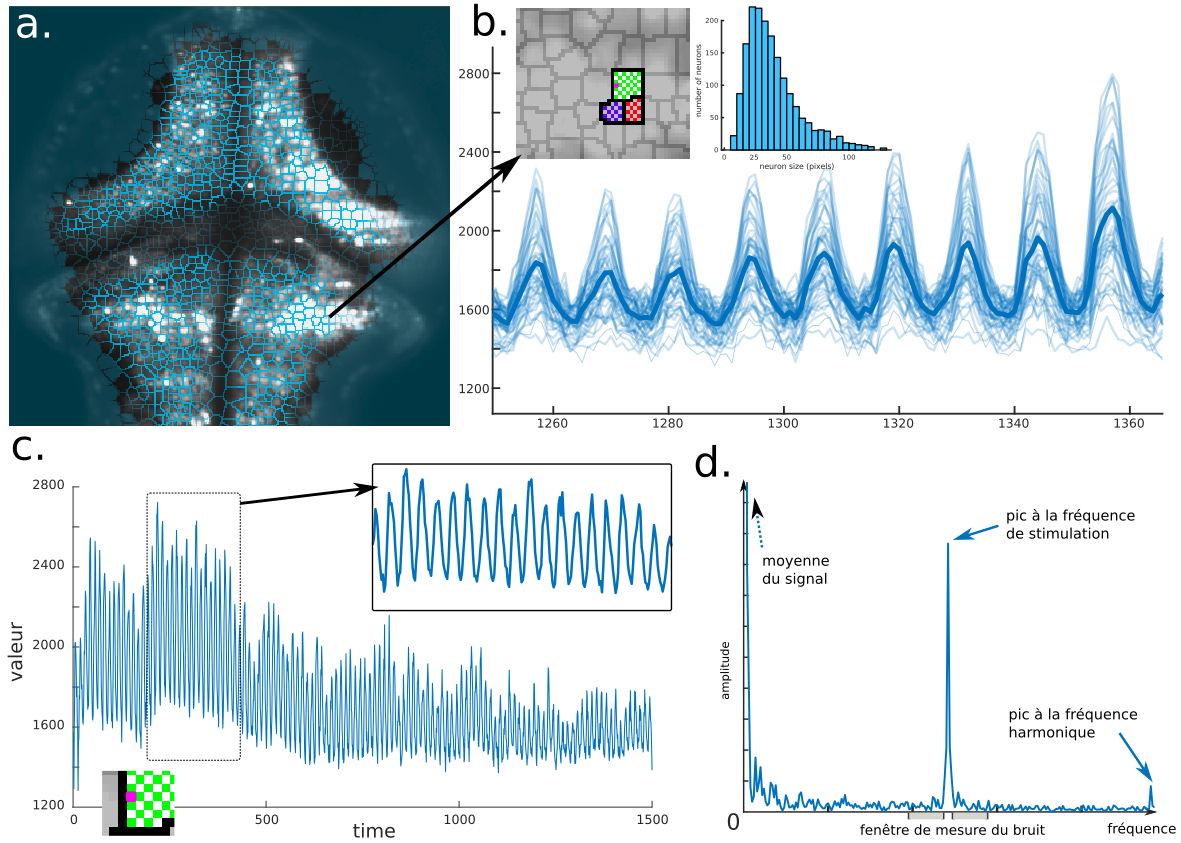
\includegraphics[width=1\textwidth]{./files/analysis_illustration.svg.png}
\caption{Illustration de différentes étapes de l'analyse.
\\a. Segmentation par l'algorithme \emph{watershed} affichée par-dessus une image moyenne.
\\b. Détail de la segmentation. Un extrait du signal du neurone en vert est affiché dessous. Chaque trait léger correspond à un pixel du neurone, le trait épais correspond à la moyenne de tous les pixels pour ce neurone. L'histogramme montre la répartition des tailles des régions pour cette couche. La plupart des segments contiennent entre 20 et 50 pixels.
\\c. Valeur de signal pour un pixel (le pixel en magenta sur le neurone vert) tout au long de l'enregistrement (le niveau de bruit de la caméra est à 400). Un détail sur la partie encadrée met en évidence son activité périodique.
\\d. Détail de l'amplitude de la transformée de Fourier discrète du signal précédent. On voit un large pic à la fréquence de stimulation, largement au-dessus du bruit évalué sur une fenêtre avoisinante.
\label{FIGfourier}}
\end{figure}    

% OK VolkerComment
% Add a figure of a typical PSD and show visually how you extract the data
% (PSD = DSP)

Il est intéressant de réaliser certaines analyses directement sur les pixels de l'image. Cela permet d'obtenir des figures avec une bonne résolution et contourne le problème de la segmentation des neurones tout en profitant au mieux de l'échantillonnage permis par la caméra. Cependant, cette approche est coûteuse en calcul, car elle opère sur un grand nombre d'éléments. Nous l'avons principalement réservée à l'analyse de Fourier pour une stimulation périodique.
Pour chaque pixel dans la région d'intérêt, on applique la transformée de Fourier discrète sur son profil temporel (cf Fig. \ref{FIGfourier} c.). Cela donne un pic en amplitude à la fréquence de stimulation et du bruit en dehors (cf Fig. \ref{FIGfourier} d.). On calcule un rapport signal à bruit comme le rapport de l'amplitude du signal sur l'amplitude du bruit moyennée sur une fenêtre autour du pic de largeur arbitraire. On considère également la phase du pic, qui représente le déphasage du signal de fluorescence avec le stimulus.
Ces valeurs pour chaque pixel sont ensuite utilisées pour représenter une couleur dans l'espace HSV (\emph{Hue, Saturation, Value} soit Teinte, Saturation, Valeur). La teinte représente le déphasage, la saturation et réglée à 1, et la valeur représente le rapport signal à bruit. 

\paragraph{Segmentation et analyse par neurone}

L'analyse par pixel est pertinente pour des études préliminaires simples, car elle est gourmande en calcul, chaque section de neurone (environ 6 µm de diamètre) étant imagée sur environ 30 pixels (pixel objet de 0.8 µm de côté) (cf histogramme Fig. \ref{FIGfourier} b.). En regroupant les pixels appartenant au même neurone, on peut réduire le volume de données à traiter tout en conservant leur qualité (cf Fig. \ref{FIGfourier} b.). Il existe de nombreux algorithmes de segmentation, certains faisant appel aux données temporelles pour tirer profit de l'activité des neurones, d'autre opérant sur l'image moyenne. Nous avons pour l'instant uniquement utilisé l'algorithme de ligne de partage des eaux (\emph{watershed}) combiné à une égalisation locale de contraste. Cela donne des résultats satisfaisants comme on le voit en figure \ref{FIGfourier} (a.).

% OK illustrer pixellation du neurone
% OK vérifier taille neurone en pixel
% TODO regarder taille de la ROI moyenne par rapport au volume total (somme du masque)

Après segmentation, on définit la valeur d'un neurone comme la moyenne des valeurs des pixels qui le constituent. Chaque segment peut représenter une partie d'un neurone, plusieurs neurones, ou même une zone de l'image sans neurones, mais beaucoup de segments représentent un neurone. Pour environ 80 000 segments, cela réduit l'échantillon à 500 Mo, ce qui permet d'appliquer des algorithmes plus gourmands en ressources en un temps raisonnable.

% TODO vérifier nombre de segments
% TODO baseline, df/f, régression...
% Z-score


% améliorations apportées
% git pour la gestion des versions
% format standard

\subsubsection{Améliorations pratiques et techniques}

\paragraph{Versionnage du code}
Le code utilisé pour l'analyse étant volumineux, sa gestion "génétique" (duplication et mutation) posait problème. J'ai donc mis en place un gestionnaire de version qui a permis d'unir les efforts de développement et de faciliter les mises à jour (correction de bugs, nouvelles fonctionnalités). Son utilisation a eu un effet positif sur la qualité du code, sa réutilisabilité, et sa prise en main. 

\paragraph{Support matériel}
Lors de l'acquisition, \href{https://hcimage.com/}{HCImage} le logiciel édité par Hamamatsu pour l'utilisation de la caméra propose deux options. L'une consiste à enregistrer en mémoire vive les images au cours de l'enregistrement et à les exporter sur le disque à la fin, l'autre consiste à enregistrer un fichier de cache au format propriétaire dcimg directement sur le disque. Dans le premier cas, la vitesse d'enregistrement ne pose pas problème, mais la taille de la mémoire vive est limitée, ce qui ne convient pas pour de longues expériences. Dans le deuxième cas, la vitesse d'enregistrement est limitante pour des images volumineuses avec une fréquence élevée, un disque dur rotatif ne convient pas et nous avons donc utilisé un disque SSD.

\paragraph{Fichier de cache}
Initialement, ce fichier de cache était converti en une collection d'images au format tiff via HCImage, qui étaient ensuite transférées sur le réseau interne depuis l'ordinateur d'acquisition vers l'ordinateur d'analyse pour enfin être traitées. Les programmes et systèmes de fichiers n'étant pas adaptés à la gestion de si nombreux fichiers, cela occasionnait un surcoût sur le temps de transfert et le temps de copie. Pour résoudre ce problème, nous sommes passés à l'utilisation directe du format dcimg. Après plusieurs tentatives infructueuses d'obtenir de la documentation auprès de l'entreprise Hamamatsu, nous avons opté pour une approche par rétroingénierie (d'autres implémentations plus complètes ont été développées par la suite comme \href{https://github.com/lens-biophotonics/dcimg}{ce module dcimg pour python}).

\paragraph{Memory mapping}
Il n'est pas envisageable de charger un jeu de données de plus de 60 Go en mémoire vive, il faut donc ouvrir les données au moment de leur utilisation. Pour obtenir une tranche d'un pixel selon (t) sur des images individuelles, il est nécessaire d'ouvrir chacune des images. Le grand nombre d'opérations de fichiers requis peut être réduit en groupant plusieurs pixels, mais au prix d'une perte de simplicité qui rend le code difficile à gérer. La solution retenue est le memory mapping, qui permet de manipuler un fichier sur le disque comme un fichier en mémoire vive, entrainant un gain de simplicité et de performance. De plus, le memory mapping permet de travailler directement sur le fichier de cache, ce qui évite des copies supplémentaires couteuses en espace et en temps.

Le memory mapping peut être combiné à l'allocation de mémoire disque pour être utilisé au moment de l'écriture. Cela facilite la manipulation des données par rapport à une écriture séquentielle dans un fichier binaire, et permet la modification d'une partie du fichier et la parallélisation de l'écriture. Pour cela, j'ai utilisé la fonction système \verb|fallocate| qui alloue de l'espace sur un disque formaté en \verb|ext4|.

\paragraph{Calcul du quantile glissant}
Une définition courante de la valeur de référence d'un signal calcique repose sur le calcul d'un quantile glissant (le huitième centile  \cite{dombeck_imaging_2007}). L'algorithme naïf qui consiste à calculer le quantile sur chaque fenêtre est inefficace ($\mathcal{O}(n^2)$), j'ai donc cherché une implémentation astucieuse et ai trouvé la fonction \verb|runquantile| de la bibliothèque \verb|caTools|, qui a apporté un gain en vitesse par rapport à l'implémentation précédente. Cette implémentation repose sur le tri par insertion mais retient le tri effectué sur la fenêtre précédente, ce qui lui permet d'atteindre une complexité en $\mathcal{O}(n\times k)$, où $n$ est le nombre de valeurs et $k$ la taille de la fenêtre.

% OK VolkerComment
% Explain the algorithm used by caTools and explain why it is faster => running quantile calculation. What is the speed gain when analyzing our data
% TOOD comparaison runquantile

% TODO temps de conversion HCImage dcimg -> tiff
% TODO temps de transfert réseau dcimg / tiff
% TODO temps de copie SSD -> SSD, HDD -> HDD

\subsubsection{Pistes d'améliorations}

\paragraph{Ordre des dimensions}
L'ordre naturel des dimensions en mémoire est l'ordre obtenu lors de l'écriture ($(x,y),z,t$). Cet ordre permet de lire et écrire rapidement une image, mais n'est pas adapté à une tranche selon $t$. En effet les valeurs à deux instant successifs pour un même pixel ($x,y,z$) sont séparées en mémoire de 12 288 000 valeurs. Lire une tranche temporelle est extrêmement long sur un disque dur rotatif et reste limitant sur un SSD. Un gain de vitesse pour des tranches temporelles peut être obtenu en permutant l'ordre des dimensions en mémoire, au prix d'une perte pour la lecture d'images (tranche $(x,y)$). Pour un ordre ($t,x,y,z$), la vitesse de lecture des images reste suffisamment rapide pour un affichage à fréquence vidéo tout en accélérant immensément la lecture de tranches temporelles, bien plus sollicitée lors de l'analyse. Réaliser ce changement nécessite une grande part de ré-écriture du code actuel et bénéficierait d'un langage plus adapté.

% TODO ressortir les benchmarks ordre dimensions

\paragraph{Réduction des données}
La taille des données brutes pourrait être largement réduite, ce qui accélérerait les copies et libérerait de l'espace disque. D'une part la dynamique des images n'exploite pas les 16 bits sur lesquels elles sont enregistrées, 12 bit suffiraient, ce qui entrainerait un gain immédiat de 25\% sur la taille des fichiers. D'autre part, la région d'intérêt ne recouvre qu'une faible part du volume enregistré, opérer sur cette région seule entrainerait un gain de 50\% environ.

% TODO estimer la taille de la ROI sur plusieurs runs

\paragraph{Langage adapté} % TODO reformuler ce paragraphe
Jusque-là, une grande partie des données ont été analysées en langage Matlab. Ce langage n'est pas très adapté à la gestion de données de ce type et souffre de plusieurs lacunes. Matlab est généralement lent, ce qui est handicapant. Matlab n'accepte de données que sur 8, 16, 32, ou 64 bits, ce qui interdit l'amélioration consistant à encoder les données sur 12 bits. Matlab est mauvais pour réaliser un système modulaire, ce qui augmente dramatiquement les efforts pour maintenir un programme. Matlab est fermé, opaque, et sous licence propriétaire, ce qui diminue les possibilités d'utilisation du code.
J'ai réalisé un prototype rapide détaillé en annexe pour évaluer l'intérêt de traiter des données en langage Julia. Le principe d'interface, et spécifiquement des \verb|AbstractArray| (\href{https://docs.julialang.org/en/v1/manual/interfaces/#man-interface-array-1}{doc}) est particulièrement adapté à la manipulation de données matricielles en memory mapping, bien plus que le \verb|memmapfile| de Matlab (\href{https://fr.mathworks.com/help/matlab/ref/memmapfile.html}{doc}) car il permet un traitement plus bas niveau tout en fournissant des abstractions plus haut niveau. Ces considérations m'ont conduit à penser que pour produire et maintenir une base de code saine et efficace pour l'analyse, il était indispensable de s'éloigner du langage Matlab, que le langage Python était une alternative possible, mais que le langage Julia était préférable. Ceci aussi bien pour une évolution à court, moyen et long terme.

% nrrd et ses limites
% 3Dslicer vs cmtk vs ants...
% dette technique sur les pipelines

% TODO VolkerComment
% SHow your test results. Be quantitative


\section{Stimulation en roulis}

Dans le papier Migault \emph{et al} \cite{migault_whole-brain_2018} nous présentons des cartes de réponse pour une stimulation vestibulaire en roulis. Une larve paralysée à l'aide de $\alpha$-bungarotoxine est placée dans le microscope, le moteur est actionné en oscillations sinusoïdales d'une amplitude de 10° à une fréquence de 0.2 Hz. Le cerveau était imagé en 20 couches à une fréquence totale de 2.5 Hz pendant 20 minutes.

% Le débit d'image est de 100 Hz intercoupé de pauses de 100 ms pour que l'actionneur piezoélectrique revienne de la dernière couche à la première couche.

\subsection{Attentes}

D'un point de vue comportemental, une larve exposée à une stimulation en roulis adopte un mouvement compensatoire des yeux et de la queue. Le mouvement des yeux (VOR, \ref{VOR}) permet de compenser les mouvements de l'environnement visuel pour conserver une vision nette. Le mouvement de la queue (VSR, \ref{VSR}) permet de corriger l'équilibre du poisson. Ces mouvements nécessitent une action musculaire pilotée par le cerveau. On pourrait donc attendre une activité dans les neurones moteurs et dans les neurones proprioceptifs. Pour étudier la réponse à un stimulus purement vestibulaire, on peut donc paralyser les poissons pour éliminer l'essentiel de cette activité.
Avec des yeux immobiles, la seule entrée visuelle restante est le mouvement de la nappe laser, à une fréquence bien plus élevée que la stimulation vestibulaire (2.5 Hz contre 0.2 Hz). Étant donné que c'est la fréquence d'acquisition, il est difficile d'estimer la réponse à ce stimulus.

Du point de vue du système vestibulaire, une stimulation en roulis est antisymétrique. En effet, quand la larve penche à gauche, l'utricule gauche est entraîné vers l'extérieur alors que l'utricule droit est entraîné vers l'intérieur. On s'attend donc à voir une activation en opposition de phase des neurones gauche et droit.

Haddon et Lewis \cite{haddon_early_1996} avaient identifié les neurones du circuit vestibulaire : les neurones afférents primaires qui relaient le signal des cellules ciliées de l'utricule jusqu'au neuropile octavo-latéral dans le cervelet, les neurones tangentiels qui poursuivent jusqu'au noyau oculomoteur contralatéral et les neurones oculomoteurs eux-mêmes. Bianco \emph{et al} \cite{bianco_tangential_2012} avaient ensuite montré l'importance pour le VOR d'une certaine classe de neurones situés dans le noyau tangentiel vestibulaire dont certaines projettent dans le noyau du faisceau longitudinal médial. Enfin, Schoppik \emph{et al} avaient trouvé des neurones vestibulaires dans les rhombomères 5 à 7 \cite{schoppik_gaze-stabilizing_2017}.

Les expériences de Favre-Bulle \emph{et al} ont permis de confirmer la présence d'activité dans les neurones cités plus haut en réponse à l'activation directe des utricules. Elles ont mis en évidence une tendance à l'excitation contralatérale et à l'inhibition ipsilatérale. En stimulant séparément l'un ou l'autre utricule, puis les deux ensemble, elles ont permis d'identifier un phénomène de superadditivité principalement localisé dans le télencéphale.

\subsection{Résultats}

\subsubsection{Carte de réponse}

\begin{figure}
\centering
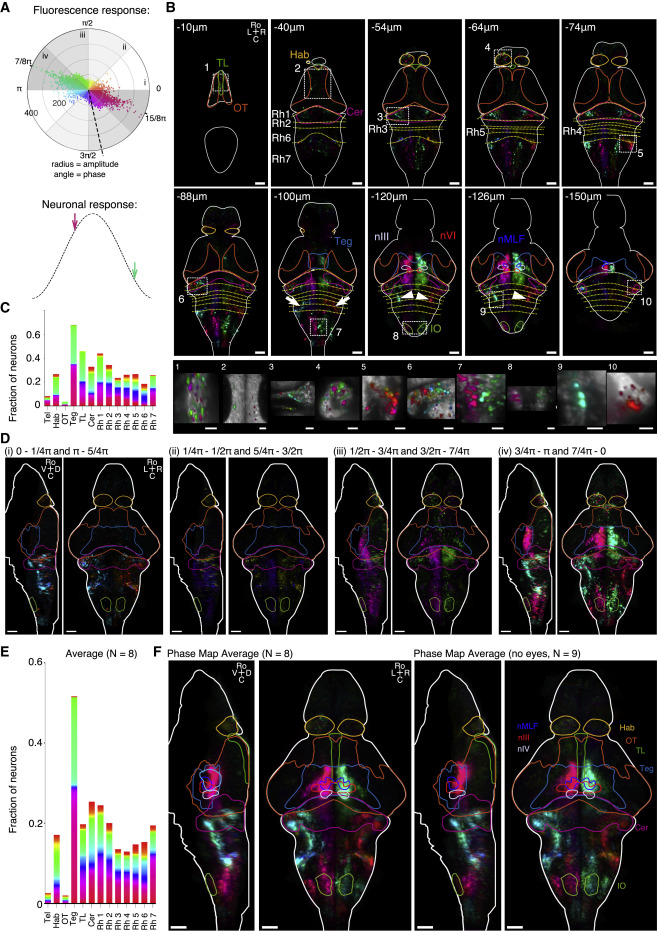
\includegraphics[width=0.95\textwidth]{./files/Migault_et-al_Fig4.jpg}
\caption{\label{FIGMigault4}} 
\end{figure}

\addtocounter{figure}{-1}
\begin{figure}
\caption{
Figure extraite du papier de Migault \emph{et al} \cite{migault_whole-brain_2018}. Cartes de la réponse fonctionnelle à une stimulation vestibulaire en roulis. Poisson paralysé exprimant le rapporteur GCaMP6s dans le noyau des neurones (elavl3:H2B-GCaMP6s).
\\\textbf{A}. Haut : réponse par neurone en coordonnées polaires. Quatre zones sont identifiées en niveau de gris (i, ii, iii, iv). La couleur indique le déphasage avec le stimulus. La ligne en pointillé indique la position attendue d'un signal à déphasage nul après correction du délai dû à un rapporteur GCaMP6s. Bas : schéma d'un cycle de stimulus, les flèches montrent le pic d'activité des neurones dont la réponse est la plus forte (en tenant en compte le délai du rapporteur calcique).
\\\textbf{B}. Haut : dix couches de la carte pour une réponse typique après alignement sur le cerveau de référence Z-Brain. Bas : agrandissement des zones encadrées par les rectangles.
\\\textbf{C}. Fraction des neurones répondant parmi les treize zones sélectionnées colorés selon leur phase.
\\\textbf{D}. Projection maximale horizontale (moitié gauche seulement) et verticale (cerveau entier) de la carte montrée en B. pour les quatre intervalles de phase identifiés en A.
\\\textbf{E}. Comme C. mais en moyenne sur huit poissons.
\\\textbf{F}. Projection maximale horizontale et verticale de la carte moyennée pour huit poissons (gauche) et neuf poissons énucléés (droite).
\\Abbréviations : \emph{Orientation} \textbf{Ro} rostral, \textbf{C} caudal, \textbf{D} dorsal, \textbf{V} ventral, \textbf{L} left, \textbf{R} right,
\\\emph{Régions}  \textbf{Hab} habenula, \textbf{IO} inferior olive, \textbf{TL} torus longitudinalis, \textbf{Teg} tegmentum, \textbf{nMLF} nuclear medial fasciculus, \textbf{nIII} oculomotor nucleus, \textbf{nIV} trochlear nucleus, \textbf{Cer} cerebellum, \textbf{Rh} rhombomere
}
\end{figure}

On voit en figure \ref{FIGMigault4} les cartes de réponse fonctionnelle du cerveau de larve pour une stimulation vestibulaire en roulis. La carte présente bien une antisymétrie bilatérale : les neurones de l'hémisphère gauche sont actifs en opposition de phase par rapport à ceux de l'hémisphère droit. Les neurones coactifs temporellement semblent être organisés en groupes colocalisés spatialement, ce qui dégage plusieurs groupes fonctionnels également symétriques.
Ces groupes sont situés dans le tegmentum, le nMLF, le noyau oculomoteur (dans le mésencéphale (nIII) et dans le rhombencéphale (nIV)), le noyau octavolatéral, le noyau vestibulaire tangantiel, le noyau vestibulo-spinal, le rhombomère 7, et l'olive inférieure. Dans d'autres régions l'activité est plus éparse : le torus longitudinalis, l'habenula, le tectum optique, le cerebellum.

\subsubsection{Déphasage de GCaMP6s}

\begin{figure}
\centering
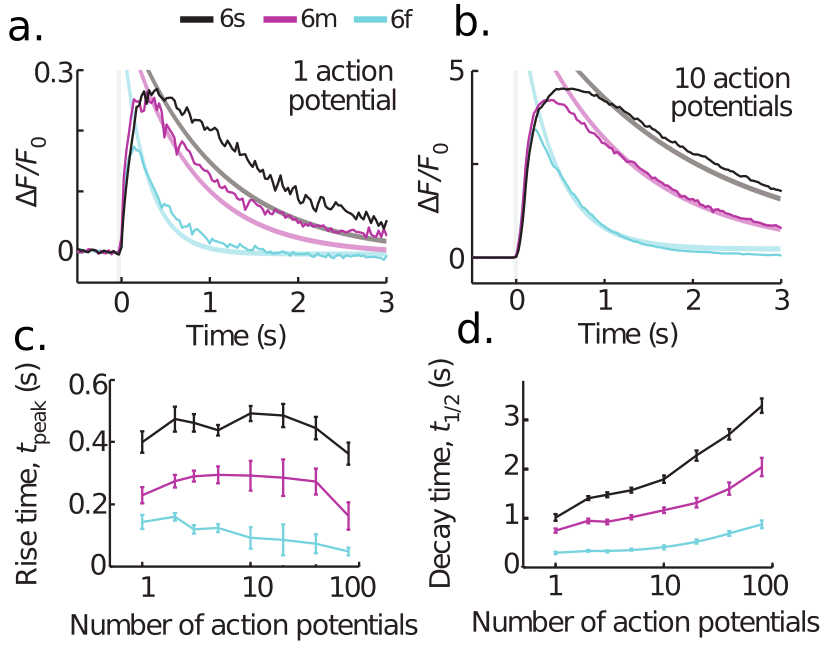
\includegraphics[width=0.8\textwidth]{./files/chen2013_GCaMP6.svg.png}
\caption{Graphiques extraits de Chen \emph{et al} \cite{chen_ultrasensitive_2013}
montrant la réponse à un train de potentiels d'action pour le rapporteur calcique GCaMP6 exprimé dans le cytoplasme pour ses trois versions (slow (s), medium (m), fast (f)). Le modèle en montée instantanée et en déclin exponentiel est ajouté sur (a.) ($\tau$ = 0.27, 0.73, 1.0) et sur (b.) ($\tau$ = 0.4, 1.16, 1.81). Les valeurs correspondent à une lecture graphique de (d.). 
\label{FIGcalciumkernel}} 
\end{figure}

On trouve des neurones à toutes les valeurs de déphasage possible, mais la plupart se situent à des valeurs de -$\pi$/8 et son symétrique, 7$\pi$/8. Cette valeur représente le décalage entre le stimulus sinusoïdal et la fluorescence mesurée. Par exemple, un déphasage de zéro correspond à un signal maximum lorsque la valeur de l'angle est maximale, c'est-à-dire une larve inclinée de 10° vers la droite. Toutefois, cela ne représente pas directement l'activité du neurone. En effet, il faut prendre en compte le décalage dû à la constante de temps du rapporteur calcique. En figure \ref{FIGcalciumkernel}, on montre la réponse d'un rapporteur calcique dans un neurone en fonction du nombre de potentiels d'action. On remarque que le modèle en déclin exponentiel résume bien la réponse dans la plupart des cas, on peut donc ignorer le temps de montée. Cependant, le temps de déclin caractéristique évolue significativement entre un seul potentiel d'action et cent potentiels d'action sans montrer de phénomène de pallier. Pour estimer le déphasage lié à la réponse du rapporteur calcique, nous avons enregistré l'activité spontanée des neurones pour plusieurs poissons et appliqué l'algorithme de déconvolution aveugle développé par Tubiana \emph{et al} \cite{tubiana_blind_2017} qui a estimé un temps de déclin de $\tau_\text{H2B-GCaMP6s-Nuclear} = 3.5 \pm 0.7 s$. Avec cette valeur de $\tau$ on approche le noyau du rapporteur calcique par :

$$
K(t) = \frac{1}{\tau}\exp\left(-\frac{t}{\tau}\right)H(t)
$$

Le signal de fluorescence $F(t)$ est obtenu comme le produit de convolution entre la concentration de calcium intracellulaire et le noyau de convolution. Comme détaillé en annexe \ref{calculdetail}, on trouve un décalage entre l'activité du neurone et le signal de fluorescence $\varphi_\text{GCaMP} = \arctan(-\omega\tau)$. Pour retrouver l'activité des neurones à partir du signal de fluorescence, on doit donc appliquer un déphasage de $ -\varphi_\text{GCaMP} = -\mathrm{atan}(-2\pi 0.2 \mathrm{Hz} \times 3.5 \mathrm{s}) = +1.35\ \mathrm{rad}$ sur le résultat de la phasemap.

\subsubsection{Discussion}

Des expériences de stimulation vestibulaire sinusoïdale en roulis permettent de cartographier l'activité du cerveau en réponse à ce stimulus. Les cartes présentent une antisymétrie bilatérale et des groupes de neurones ayant une réponse temporelle et un emplacement proche. On retrouve notamment les neurones des circuits vestibulaires connus liés à la stimulation des utricules et aux réflexes liés. Cette analyse constitue un échantillon de la réponse fréquentielle à une fréquence déterminée (0.2 Hz), elle pourrait être poursuivie pour d'autres fréquences. Une autre piste est d'explorer la réponse impulsionelle avec une stimulation en escalier. Cette stimulation est également présentée dans le papier, accompagnée d'une analyse par régression, mais je ne la détaille pas ici. Je m'intéresserai plutôt à reproduire une carte similaire, mais adressée à la réponse en tangage.


\section{Stimulation en tangage}\label{SECTIONtiltmicroscope1P}
% Adaptation en tilt, illumination par derrière ?

Nous avons vu dans la section précédente la réponse à une stimulation en roulis pour ce premier microscope. Dans l'objectif de comprendre les mécanismes neuronaux responsables du contrôle postural en tangage, et en prévision de l'étude en deux photons, une deuxième version a été développée, c'est celle sur laquelle j'ai travaillé. Je présente dans cette section les cartes de réponse pour une stimulation sinusoïdale en tangage et les compare avec les cartes précédentes obtenues en roulis, mais avant ça, le montage qui les a permises.

\subsection{Description du montage}

\begin{figure}
\centering
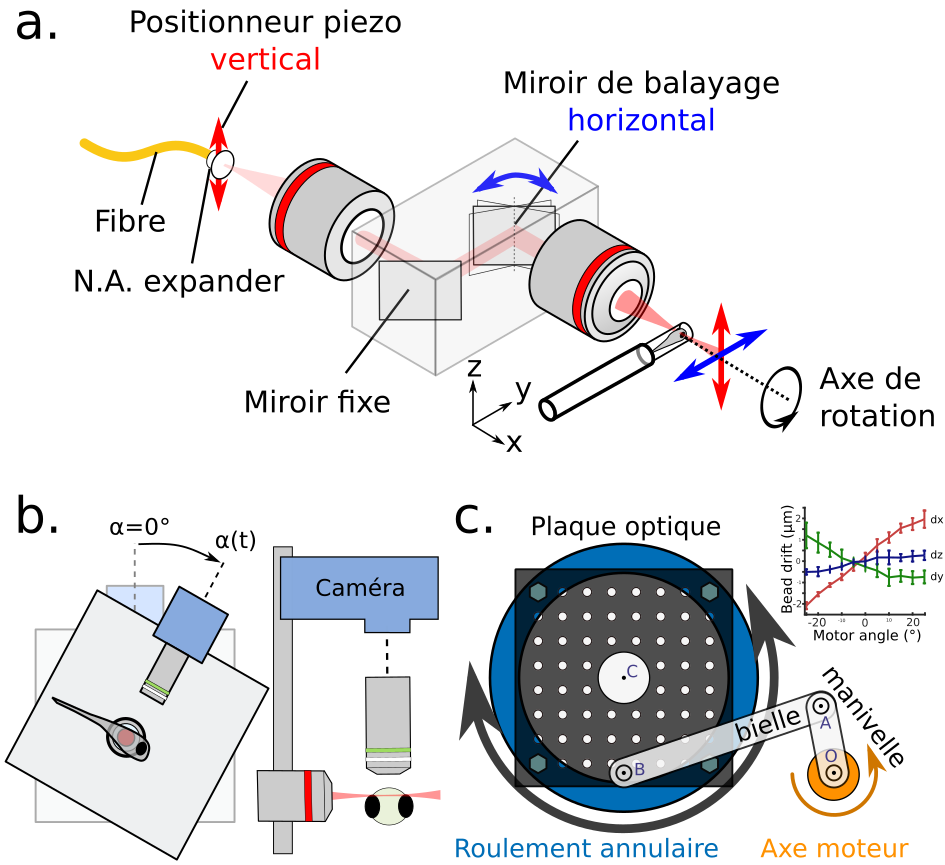
\includegraphics[width=0.8\textwidth]{./files/miniature_light-sheet_tilt.svg.png}
\caption{Microscope rotatif conçu pour la stimulation en tangage.
\\a. Module de balayage adapté avec un miroir fixe. La fibre arrive dans la même direction que l'axe de rotation.
\\b. Schéma du montage. L'unité d'illumination est fixée sur une plaque optique qu'elle traverse. La fibre arrive par derrière la nappe laser ressort par devant, du côté de l'échantillon. Le module de détection est fixé par-dessus l'échantillon.
\\c. Un système bielle-manivelle entraîne la plaque optique fixée à un roulement annulaire. La position de l'axe moteur (O) est réglable et permet une oscillation sinusoïdale (au niveau de B, la longueur OA permet de régler l'amplitude) ou un mouvement circulaire (au niveau de C, avec une manivelle de longueur BC). La stabilité du système en fonction de l'angle est indiquée en encart.
\label{FIGtiltlightsheet}}
\end{figure}

Pour une stimulation en tangage, le poisson doit être placé perpendiculairement à l'axe de rotation, avec les deux oreilles internes sur l'axe. Le laser devant arriver par le côté, le module de balayage a été adapté avec un miroir fixe pour que la direction d'entrée et de sortie soient parallèles. Ainsi, la fibre peut être placée le long de l'axe de rotation, ce qui minimise ses déformations.

Pour tourner la plateforme, un moteur pas à pas actionne à travers un réducteur un système bielle manivelle fixé à la plaque optique sur laquelle est fixée les différents éléments du microscope (cf Fig. \ref{FIGtiltlightsheet}). La stabilité du système a été caractérisée par la méthode détaillée en figure \ref{FIGbeadstability} et présente les mêmes caractéristiques (excellente stabilité en z, stabilité horizontale raisonnable pouvant être facilement corrigée \emph{a posteriori}).

L'entrée de fibre se fait au moyen d'un connecteur FC/PC (\emph{Fiber Connector with Physical Contact}) qui permet de changer facilement de fibre tout en conservant l'alignement. Pour les fibres ayant une ouverture numérique faible, une lentille placée en sortie de fibre permet d'adapter l'ouverture numérique du faisceau et ainsi de couvrir l'ensemble de la pupille d'entrée de l'objectif d'entrée du module de balayage. Les premières acquisitions un photon ont été réalisées à l'aide d'une fibre monomode identique à celle du microscope précédent.

\subsection{Carte de réponse comparée}

\begin{figure}
\centering
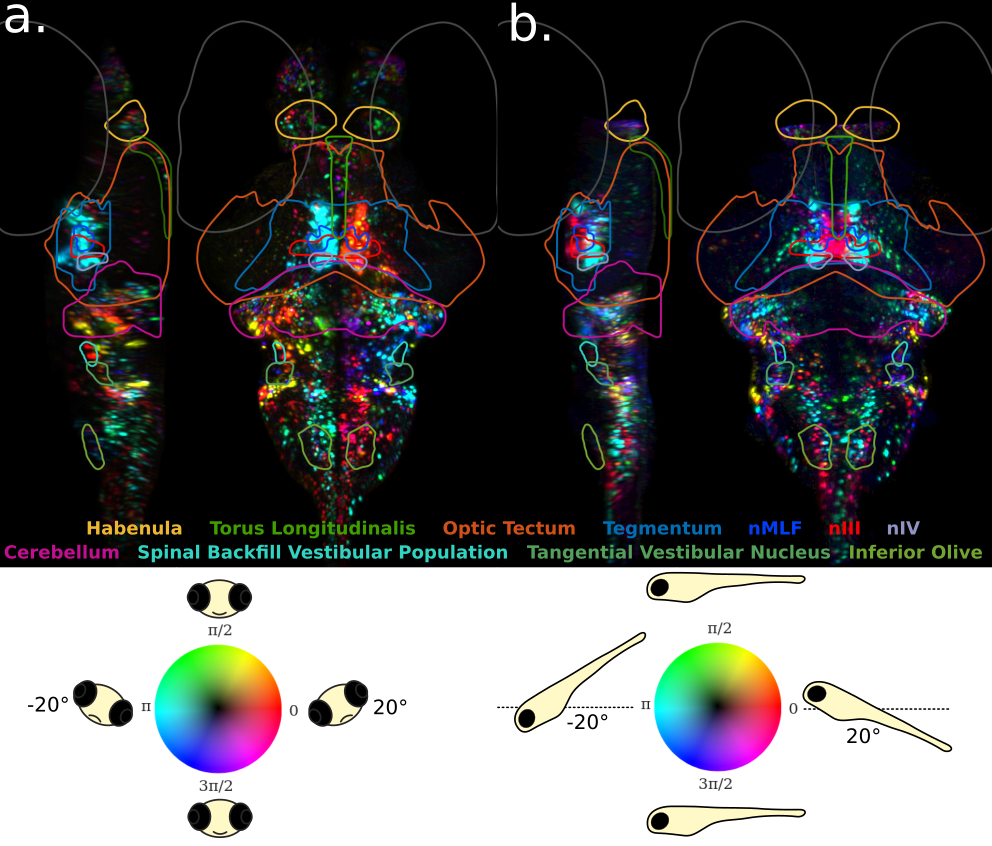
\includegraphics[width=\textwidth]{./files/tilt_roll.svg.png}
\caption{Cartes de réponses obtenues pour une stimulation de rotation sinusoïdale selon l'axe de roulis (a, premier microscope) et de tangage (b, second microscope). On remarque que la carte est antisymétrique dans le cas du roulis et symétrique dans le cas du tangage.
Pour le roulis, la vue de côté est réalisée sur la moitié gauche du volume seulement.
\label{FIGtiltroll}}
\end{figure}

En figure \ref{FIGtiltroll}, je montre côte à côte une des cartes de réponse en roulis présentées dans la section précédente et une carte en tangage obtenue sur ce second microscope (en acquisition un photon). L'observation la plus évidente est que la carte en tangage présente une symétrie bilatérale. En effet, les deux utricules sont activés exactement en même temps avec la même amplitude par la rotation de la larve. Les phases les plus représentées (rouge et cyan) sont les mêmes que pour la carte en roulis, ce qui confirme que les neurones sont excités par le même type de stimulation (mélange de vitesse et de position). La zone qui présente le plus d'activité est également le noyau oculomoteur nIII et nIV. On distingue cependant une différence avec la carte en roulis : alors que tous les neurones situés du même côté du tegmentum sont en phase dans la stimulation en roulis, on remarque deux zones en opposition de phase dans la simulation en tangage. Ces deux zones peuvent être séparées en deux par un plan horizontal. La zone dorsale recouvre à la fois le nMLF, et le noyau oculomoteur nIII et nIV. La zone ventrale recouvre surtout le nMLF et nIII. Des zones plus rostrales semblent aussi actives comme un cluster de neurones glutamatergiques du mésencéphale (région 111 de l'atlas zbrain) et une bande d'oligodendrocytes du diencéphale (région 043 de l'atlas zbrain). Cela est cohérent avec les connaissances actuelles sur les neurones oculomoteurs \cite{schoppik_gaze-stabilizing_2017} et l'activation des muscles oculaires pendant le VOR.

Une autre observation un peu moins évidente est la répartition des phases. En roulis, elle est parfaitement symétrique, car une inclinaison à gauche est équivalente à une inclinaison à droite. En tangage, par contre, une incliniaison négative (tête vers le bas) semble générer plus d'activité qu'une inclinaison positive (tête vers le haut). Cela se traduit par un excès de cyan/vert sur la carte de phase par rapport au rouge/magenta. On peut rapprocher cette observation de l'instabilité naturelle de la larve : alors qu'elle est en équilibre instable gauche/droite, elle est en déséquilibre en tangage. Ehrlich et Schoppik ont même suggéré que ce déséquilibre était à l'origine de l'initiation du mouvement \cite{ehrlich_control_2017}.

\subsection{Conclusion}

Ce nouveau microscope a permis de réaliser la cartographie du cerveau en réponse à une stimulation vestibulaire en tangage en répondant aux exigences de stabilité. Toutefois, avant de s'en servir pour réaliser un environnement de réalité virtuelle capable de reproduire les expériences présentées en partie \ref{chapII}, il faut gagner le contrôle sur l'environnement visuel et passer d'une excitation un photon à une excitation deux photons. C'est l'objectif du chapitre suivant, dans lequel je présente les enjeux d'une feuille de lumière deux photons rotative et les solutions techniques mises en œuvre pour la réaliser.
\chapter{Microscope à feuille de lumière deux photons rotatif}

Pour étudier à la fois le système visuel et le système vestibulaire du poisson zèbre, une possibilité est de combiner les deux innovations précédemment citées en un seul microscope : un microscope à feuille de lumière deux photons rotatif. C'est la voie que j'ai explorée, qui a révélé plusieurs défis techniques. Le premier et de guider le laser deux photons vers le module light-sheet en restant stable lors de la rotation du microscope. Le second est de mitiger l'effet de lentille thermique lié à la propagation d'un faisceau haute puissance dans l'eau. Après avoir exploré en détail ces aspects techniques, je montrerai comment le microscope a permis de réaliser l'acquisition du cerveau de la larve sans environnement visuel parasite.

\section{Fibre optique, principe et état de l'art}

Dans un microscope statique, la source laser peut être guidée jusqu'à l'échantillon par des miroirs, mais dans un microscope mobile il faut soit embarquer la source laser directement sur le microscope, soit la guider de manière flexible quelque soient les mouvements. Dans le cas d'une source laser deux photons très volumineuse, il est impossible de l'embarquer, la solution adoptée est donc une fibre optique adaptée. De telles fibres optiques capables de guider un laser deux photons sont complexes à produire. Avant de nous intéresser aux microscopes à fibre couramment utilisés dans la recherche sur le rongeur, introduisons les caractéristiques d'un guide d'onde. 

\subsection{Guide d'onde}

Un guide d'onde est un objet contraignant l'onde à se propager dans une seule dimension. Pour les ondes électromagnétiques dans les fréquences radio, cela peut être réalisé avec des parois métalliques. Dans le cas de la lumière visible, on utilise généralement une âme d'indice optique supérieur à l'indice du milieu environnant. Le phénomène de réflexion totale sur le dioptre permet alors le guidage de l'onde. De telles fibres optiques sont réalisées avec un fin fil de verre et servent en télécommunication, en éclairage, en imagerie...

Nous disposons notamment de fibres monomodes qui permettent de transmettre le mode fondamental d'un laser d'un bout à l'autre sans dénaturer le profil gaussien. Nous utilisons ce genre de fibre pour guider le laser dans la version un photon du microscope à feuille de lumière rotatif.

Dans le cas d'un laser pulsé utilisé en microscopie deux photons, les fibres à milieu d'indice fonctionnent également mais ont un inconvénient majeur qui les rend inutilisables telles quelles pour cette application dû au phénomène de dispersion. Un laser pulsé a contient d'autant plus de longueurs d'ondes que son pic est étroit.

$$
\Delta \lambda_t = \frac{\lambda^2}{c}\Delta\nu_t
$$

Dans un milieu dispersif, ces différentes longueurs d'onde se propagent à une vitesse différente, ce qui donne lieu à un élargissement de l'impulsion. L'effet deux photons étant lié quadratiquement à la puissance instantanée, il chute de manière critique avec la dispersion. Une solution est de précompenser cette dispersion via des éléments optique positionnés avant l'injection dans la fibre comme une suite de prismes. Cette solution permet de réduire la largeur temporelle du pic en sortie de fibre pour des puissances relativement faibles, mais pas pour de fortes puissances, pour lesquelles l'automodulation de phase liée à l'effet Kerr optique devient dominant. C'est pourquoi il vaut mieux un guide d'onde non dispersif.

\subsection{Fibre à âme creuse}

Un milieu non dispersif commun est le vide, d'où l'idée de construire un guide d'onde à cœur creux. L'effet de réflexion totale sur le dioptre ne peut plus être utilisé, car il faudrait un milieu d'indice plus petit que 1, c'est à dire dans lequel la lumière se propage plus vite que dans le vide, ce qui n'est pas possible. Une idée consiste donc à utiliser un phénomène de réflexion par interférences comme le miroir de Bragg. Un tel miroir est constitué d'une succession périodique de couches d'indice différents et permet d'obtenir une réflexion quasi totale à la longueur d'onde du motif. On trouve ce genre de réseau dans des fibres microstructurées \cite{argyros_hollow-core_2006}.

Cette idée a également donné lieu aux fibres à réseau trihexagonal, ou "Kagomé". De telles fibres ont été construites pour la première fois en 2002 sous le nom de fibre à cristaux photoniques en étirant un réseau de capillaires. Le gain était alors de l'ordre de 2 dB/m \cite{benabid_stimulated_2002}. En 2011, un gain de 180 dB/km a été obtenu avec de telles fibres \cite{wang_low_2011}. Un des problèmes des fibres à structure géométrique est la sensibilité aux déformations. Puisque le guidage est lié à la géométrie de la fibre, les déformations qui changent cette géométrie altèrent le guidage. Cela peut prendre la forme de perte de transmission, de couplage entre les modes, d'incidence sur la polarisation. Mais cette sensibilité aux déformations dépendant de la géométrie de la fibre, certaines configurations donnent des résultats très satisfaisants.

\begin{figure}
\centering
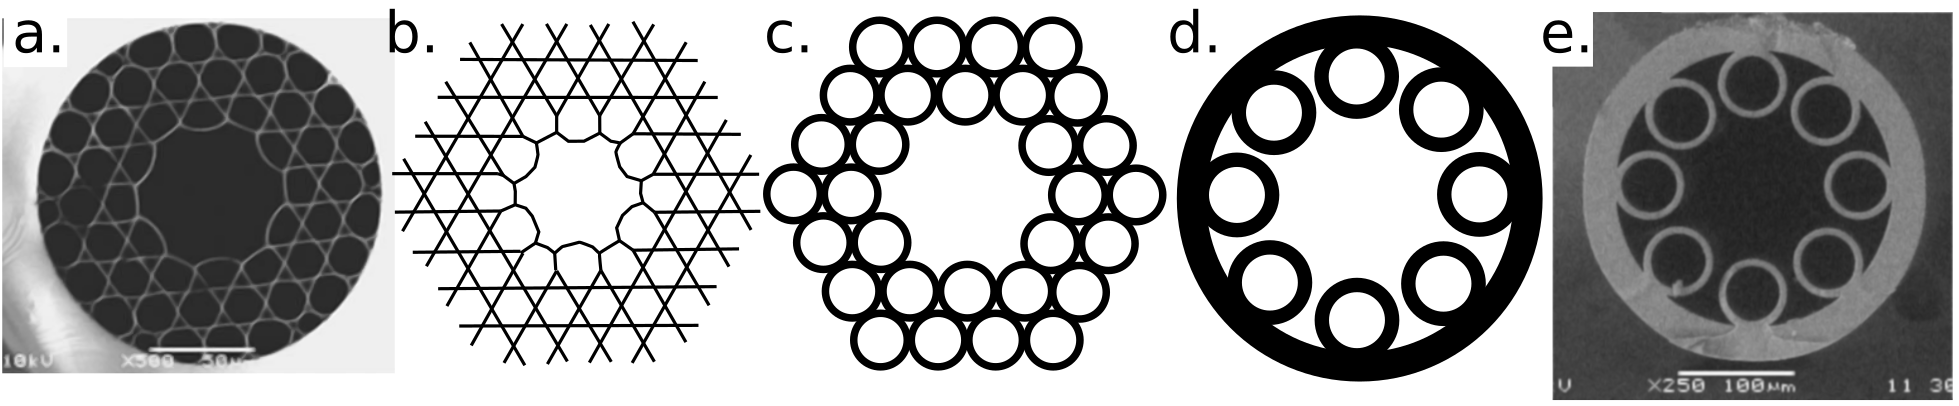
\includegraphics[width=1\textwidth]{./files/fibers.svg.png}
\caption{Illustration de différents types de fibres évoquées.\\
a. Fibre Kagomé (image extraite de Wang 2011 \cite{wang_low_2011}) \\
b. Schéma du motif Kagomé\\
c. Schéma d'un réseau tubulaire comme dans Vincetti 2010 \cite{vincetti_waveguiding_2010}\\
d. Schéma d'une fibre à courbure négative\\
e. Fibre à courbure négative (image extraite de Yu 2016 \cite{yu_negative_2016})\\}
\end{figure}

Le processus de fabrication de ces fibres à réseau trihexagonal a très naturellement donné lieu à des fibres à "réseaux de tubes" qui ont révélé avoir de bonnes performances. L'analyse numérique de leur fonctionnement a révélé que la première couche du réseau de tube jouait un rôle important dans leurs propriétés \cite{vincetti_waveguiding_2010}, ce qui a permis l'apparition des fibres à "courbure négative", avec une géométrie très simple et de très bonnes caractéristiques. C'est cette configuration qui nous intéresse ici. Nous l'avons retenue pour sa large bande de transmission qui couvre à la fois le visible à 488 nm et l'infrarouge à 915 nm, son bon gain de ~100 dB/km, son couplage monomode dans l'infrarouge et sa relative stabilité par rapport aux déformations.

\subsection{TODO Utilisation des fibres optiques en microscopie embarquée}

- review rongeur

\section{Caractérisation et utilisation de la fibre PMC-C-9005 B2}

La fibre que j'ai utilisé pour coupler le laser femtoseconde dans notre microscope est un modèle de recherche et développement réalisé par l'entreprise \href{http://www.glophotonics.fr/}{Glophotonics}. Je commente ici certaines caractérisation fournies par le constructeur et y apporte des éléments supplémentaires relativement à la polarisation.

\begin{figure}
\centering
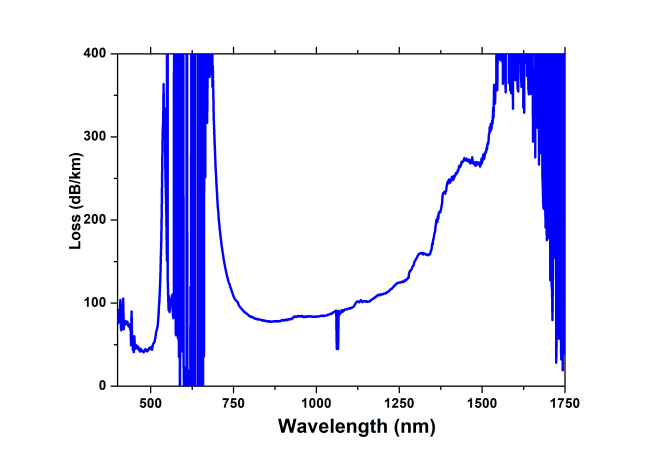
\includegraphics[width=0.8\textwidth]{./files/fiber_gain.png}
\caption{Ce spectre de transmission de la fibre PMC-C-9005 B2 a été réalisé en lumière blanche. Il montre deux zones de transmission, l'une autour de 500nm, l'autre entre 800 nm et 1200 nm. Le gain y est autour de 100 dB/km, soit une transmission d'environ 97\% à travers un mètre de fibre.}
\end{figure}

Une des particularités de cette fibre est sa large bande passante qui lui permet de transmettre à la fois de la lumière visible et de la lumière infrarouge. Dans mon cas, je l'utilise à la fois à 488 nm pour l'imagerie un photon et à 915 nm pour l'imagerie deux photons.

\subsection{Injection d'un laser dans une fibre}

Pour injecter le laser dans la fibre, il faut aligner tous les éléments dans l'axe optique et régler finement les degrés de liberté en translation et en rotation. De plus, comme on souhaite un couplage monomode, il faut faire coincider le mode laser d'entrée de fibre avec le mode propre de la fibre. Le laser ayant un largeur initiale de D, il faut le ramener à une largeur de fibre $\omega$ (23 $\mu m$ ± 1 $\mu m$ d'après la documentation). Pour cela, il faut utiliser une lentille de focale f et satisfaire l'équation suivante :

$$
f = D\frac{\pi\omega}{4\lambda}
$$

\subsection{Injection 2P}

Le laser "Mai-Tai" que j'ai utilisé est proche d'un faisceau gaussien (M²<1.1) et son waist (w0) est large d'environ 1 mm. Ces valeurs sont données par la documentation pour une utilisation à 800 nm, mais elles peuvent évoluer légèrement en accordant la longueur d'onde de fonctionnement.

La largeur d'un faisceau gaussien est définie par la fonction :

$$
w(z) = w_0 \, \sqrt{ 1+ {\left( \frac{z}{z_\mathrm{R}} \right)}^2 }
$$

avec

$$
z_\mathrm{R} = \frac{\pi w_0^2 }{\lambda}
$$

La largeur du laser est donc d'environ 2 mm après un mètre de propagation. En prenant D = 2 mm, $\omega$ = 23 $\mu m$, et à $\lambda$ = 915 nm, on trouve donc f = 40 mm, c'est pourquoi j'ai utilisé une lentille de focale 40 mm (référence Thorlabs AC254-040-B-ML). Cette lentille dispose également d'un traitement de surface pour optimiser la transmission dans l'infrarouge.

J'ai fixé une extrémité de la fibre sur une platine de translation xyz à 40 mm de la lentille. Pour faciliter l'alignement, j'ai tout d'abord injecté un laser visible grâce à un connecteur fibre à fibre dans l'autre extrémité. Cela m'a permis de pré-aligner deux miroirs sur support rotatifs en visant l'orifice du laser parallèlement à l'axe optique. En allumant le laser à faible puissance pour ne pas endomager la fibre, j'ai donc obtenu facilement une transmission suffisante pour pouvoir mesurer la puissance en sortie de fibre. À partir de cette étape, il suffit d'optimiser la puissance transmise en jouant sur les réglages. Dans un premier temps, les deux degrés de rotations de chacun des deux miroirs, et dans un deuxième temps, les deux degrés de rotation du second miroir et les trois degrés de translation de la platine. Cette technique permet d'obtenir en un temps raisonnable (~1h) une transmission optimale (~96\%).

\begin{figure}
\centering
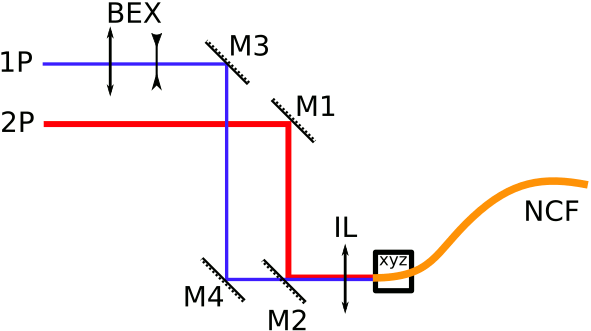
\includegraphics[width=0.8\textwidth]{./files/injection.svg.png}
\caption{schéma de l'injection à deux lasers dans la fibre. Le miroir M2 est amovible et permet de basculer entre l'injection 1P et 2P}
\end{figure}

\subsection{Injection 1P}

Pour injecter un deuxième laser, il faut à nouveau faire coïncider le mode de la fibre avec celui du laser, mais en conservant la même lentille d'injection et sans utiliser la platine de translation. Il faut donc adapter la largeur du faisceau à l'aide d'un téléscope ou beam expander (BEX). En remplaçant 915 nm par 488 nm, on obtient D = 1 mm. La lentille étant optimisée pour l'infrarouge, sa transmission dans le bleu n'est que de 50\%, mais la puissance du laser bleu est suffisante pour compenser cette perte. Par contre, la fibre n'est pas tout à fait monomode à cette longueur d'onde, et l'on distingue clairement en sortie le mode TEM11 ou les modes TEM10 / TEM01 en fonction de la position de la fibre. La meilleure transmission obtenue est de l'ordre de 50\%, mais cela est suffisant pour l'imagerie statique (fibre immobile).

\subsection{Dispersion et pré-compensation}

Un paramètre important pour la transmission d'un laser pulsé est la dispersion. C'est celui qui nous force à utiliser des fibre à cœur creux et qui permet de conserver une impulsion aussi courte que possible. Mais la dispersion d'une fibre à cœur creux n'est pas nulle, elle est de l'ordre de 1 ps/nm/km (élargissement temporel / largeur spectrale / distance parcourue) comme on peut le voir sur la courbe.

\begin{figure}
\centering
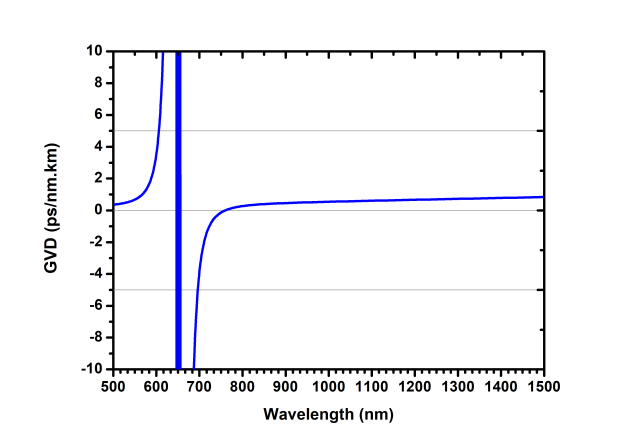
\includegraphics[width=0.8\textwidth]{./files/fiber-dispersion.png}
\caption{profil de dispersion de la fibre PMC-C-9005 B2}
\end{figure}

La largeur spectrale d'une impulsion est donnée par

$$
\Delta \lambda_t = \frac{\lambda^2}{c\Delta t}
$$

et vaut donc 28 nm. Pour une impulsion de 100 fs à 915 nm, cela donne un élargissement de l'ordre de 28 fs au bout d'un mètre de propagation dans la fibre, soit une perte de concentration de 30\% et donc une perte d'effet deux photons de 50\%. Heureusement, il est possible de pré-compenser cette dispersion à l'aide d'un système optique placé en amont de la fibre. Le laser "Mai-Tai" est justement accompagné d'un élément "Deepsee" qui permet une telle précompensation réglable de -8 900 à -24 500 fs² d'après la documentation.

> The amount of dispersion, or GVD compensation, provided for each wavelength depends on the position of the DeepSee motor that moves optical material on a stage within the beam path.

En mesurant la durée de l'impulsion en sortie de fibre à l'aide d'un autocorrélateur, on confirme que la précompensation permet de retrouver une impulsion de 100 fs dans l'échantillon.

\subsection{Gain de courbure}

Un des facteurs qui peut affecter la transmissission de la fibre est sa courbure. Certaines fibres comme les fibres à cristaux photoniques Kagome sont très sensibles à la courbure. La première fibre que j'ai testée voyait ainsi varier sa transmission d'un facteur un à cinq en fonction de sa courbure. Puisque la rotation du microscope engendre des déformations de la fibre, on se retrouve avec un éclairage incident corrélé à la stimulation, ce qui crée un signal parasite. Si ce signal parasite dépasse environ 1\%, le rapport signal à bruit devient trop faible, et les données ne sont plus analysables. Pour caractériser les pertes de transmission liées à la courbure, il suffit de placer un puissance-mètre en sortie de fibre et de faire varier la courbure.

Des modèles numériques \cite{yu_negative_2016} \cite{setti_flexible_2013} et des applications pratiques suggèrent que le gain évolue de manière inversement proportionelle au carré du rayon de courbure. J'ai observé la même tendance sur notre fibre.

\begin{figure}
\centering
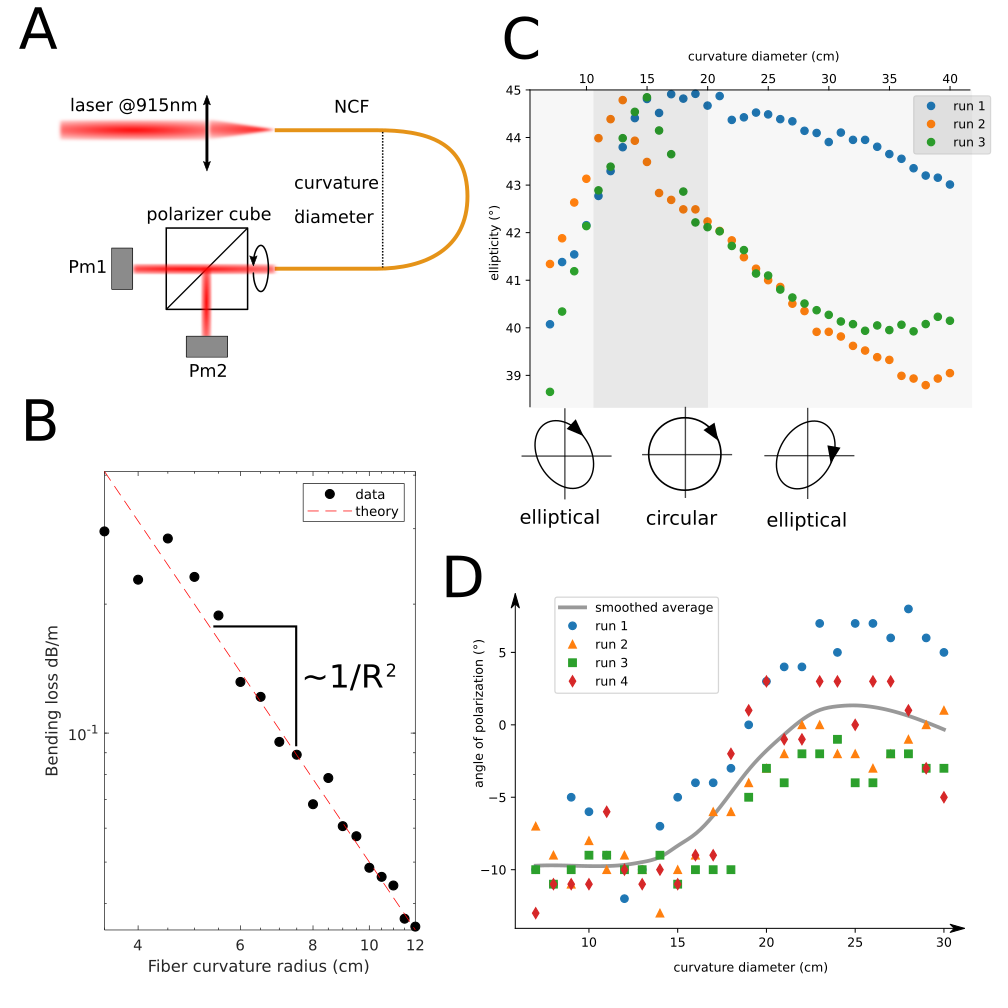
\includegraphics[width=0.8\textwidth]{./files/fiber_bending.png}
\caption{A. schéma du setup de catactérisation
\\ B. gain en fonction de la courbure
\\ C. ellipticité en fonction de la courbure (quasi circulaire)
\\ D. angle de polarisation en fonction de la courbure (quasi linéaire)}
\end{figure}



On constate que le gain lié à la courbure est bien similaire au modèle théorique. Les pertes par mètre de fibre restent cependant petites car autour de 0.1 dB (~2\%) même pour un rayon assez court de 7 cm. De plus, un rayon de courbure si court est rarement atteint sur une longue section de fibre. Dans le pire des cas la fibre peut effectuer un 'U' de 5 cm de rayon sur une longueur de $\pi$ × 5 cm soit 16 cm maximum, ce qui correspond à une perte inférieure à 5\%, mais il est facile d'éviter cette situation en positionnant la fibre correctement. 

\subsection{Polarisation}

Quand l'axe d'excitation est dans la même direction que l'axe d'observation, la polarisation incidente importe peu car le dipôle (l'échantillon, en l'occurence le fluorophore) oscille dans le plan orthogonal. Mais quand les deux sont perpandiculaires, tourner la polarisation peut faire varier la lumière collectée de 0 à 100\%.

\begin{figure}
\centering
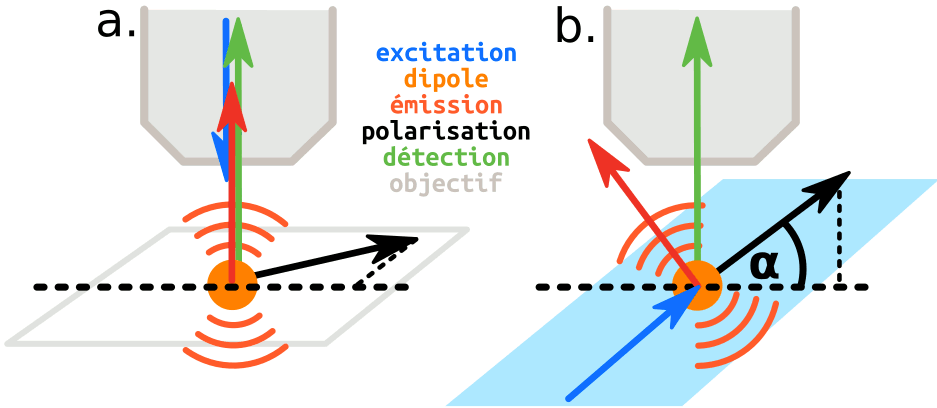
\includegraphics[width=0.8\textwidth]{./files/polarization_plane.svg.png}
\caption{a. Comme dans un microscope deux photons classique, la direction d'émission et de détection sont alignées, et la polarisation est dans le plan orthogonal. Quelle que soit la polarisation, la lumière détectée est toujours la même.
\\ b. Dans un microscope à feuille de lumière, la direction d'émission est dans le plan orthogonal à la détection. La direction de polarisation fait alors un angle $\alpha$ avec la direction de détection. Pour $\alpha$ = 90°, la lumière détectée est maximale, mais pour $\alpha$ = 0°, elle est nulle.}
\end{figure}


Il est donc important de caractériser le comportement de la fibre par rapport à la polarisation. Deux cas sont donc à envisager : une rotation de la polarisation et un changement d'ellipticité. En mesurant l'orientation de la polarisation en sortie de fibre, j'ai montré que celle-ci pouvait tourner largement en fonction de la courbure de la fibre. Par exemple, entre un rayon de courbure de 15 cm et 25 cm, une polarisation linéaire peut tourner de 10°. À cause de l'anisotropie du rayonnement dipôlaire, une polarisation tournée de 90° fait chuter le signal de 100\%. Une rotation de 10° fait chuter le signal de 17\%. En pratique, il est difficile de mainenir la fibre parfaitement droite, et donc de minimiser la rotation de la polarisation, c'est pourquoi j'ai cherché à obtenir une polarisation invariante par rotation, c'est-à-dire une polarisation circulaire.

En polarisation circulaire, la rotation n'est plus un problème, mais la fibre peut toujours transformer la polarisation circulaire en une polarisation elliptique, qui perd sa symétrie et devient donc sensible à la rotation. J'ai donc caractérisé la variation d'ellipticité dans le cas d'une polarisation circulaire. Pour cela, j'ai positionné deux puissance-mètre sur les bras d'un cube polariseur en sortie de fibre. Pour chaque courbure de fibre, je mesurais l'intensité minimale et l'intensité orthogonale, ce qui permet de déduire le grand axe (a) et le petit axe (b) de l'ellipse, et donc l'ellipticité ($\theta$) définie par

$$
\tan(\theta)=\frac{b}{a} 
$$

Je montre que l'ellipticité peut varier de 5° entre deux courbures extrêmes. Pour une polarisation elliptique à 40°, la différence entre grand axe et petit axe est de 16\%. Une rotation de 90° en polarisation elliptique avec cette ellipticité donnerait alors lieu à une variation de détection de 16\%, ce qui est beaucoup mieux que 100\%. Il est cependant nécessaire d'effectuer des tests en conditions réelles afin de vérifier que ce pire cas n'est pas atteint.

\subsection{Test en conditions réelles}

Pour tester les variations d'intensité dues aux déformations de la fibre en conditions réelles, j'ai monté un cube polariseur et un puissance-mètre à la place de l'échantillon et ai soumis l'ensemble à des stimulations périodiques guidées par un moteur.

\begin{figure}
\centering
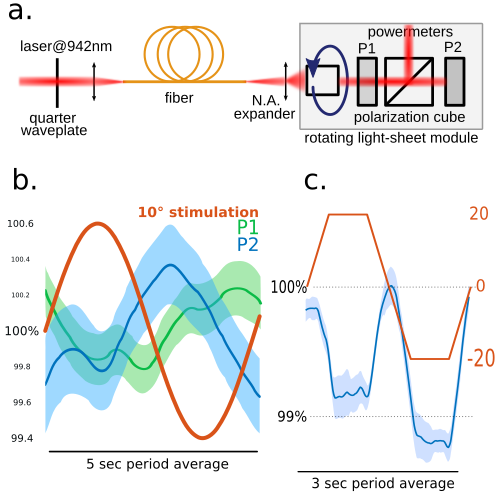
\includegraphics[width=0.8\textwidth]{./files/real-condition_intensity-variation.png}
\caption{
\\ a. Setup de test en condition réelle
\\ b. Réponse à une stimulation sinusoïdale périodique de 10°. On constate que les variations de puissance ne dépassent pas 0.6\% et que ces variations combinées aux changement de la polarisation (ellipticité et rotation) n'excèdent pas 1.2\%.
\\ c. Réponse à une stimulation périodique en marches de 20°. Les variations combinées n'excèdent pas 1.2\%. On remarque que l'intensité maximale est atteinte pour un angle du moteur de 0°, soit la position de repos de la fibre.
}
\end{figure}

Finalement, tous les effets liés à la position de la fibre engendrent des variations de l'intensité détectée inférieurs à 1.2\% dans les conditions des expériences. Les effets parasites sont donc connus et mineurs, ce qui est à prendre en compte lors de l'analyse des données.

\section{Effet deux photons}

L'absorption à deux photons est un phénomène non linéaire qui est négligeable aux petites énergies mais devient important pour une intensité lumineuse élevée. Elle peut se produire entre deux ondes de fréquence différente, mais on s'intéresse au cas particulier de deux ondes fréquences égales. Cet effet est proportionnel au carré de l'intensité lumineuse et est lié au caractère anharmonique du dipôle oscillant.

\begin{figure}
\centering
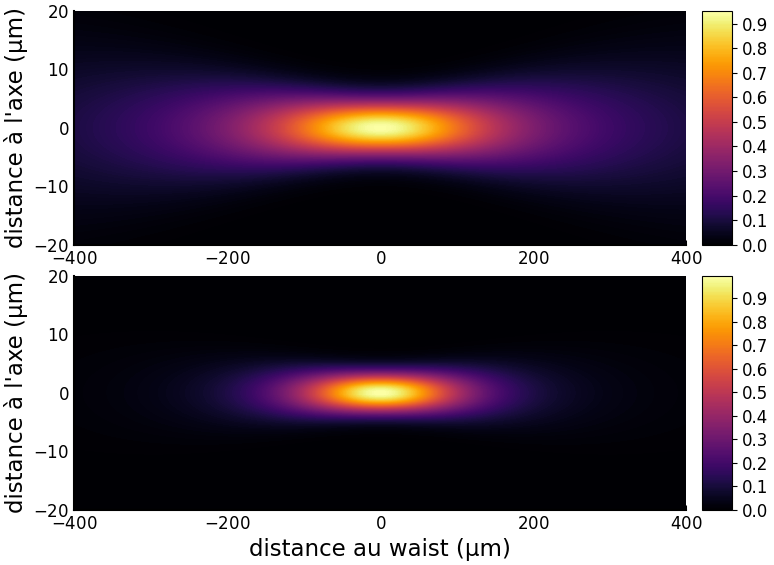
\includegraphics[width=0.8\textwidth]{./files/profile-intensity.png}
\caption{
comparaison du profil d'intensité (haut) et de son carré (bas). On voit que la zone concernée par l'effet deux photons et restreinte. (paramètres : indice optique 1.33, longueur d'onde 915 nm, waist 6.5 $\mu m$)
}
\end{figure}

La zone concernée par l'effet deux photons est donc restreinte. C'est un avantage dans la direction verticale, car cela permet un meilleur sectionnement optique (en particulier au bord, où la largeur du faisceau est supérieure à la taille d'un neurone), mais c'est également un inconvénient dans la direction de propagation, car la baisse d'intensité de part et d'autre du waist est plus importante (on le verra sur les images).

Une grande intensité étant nécessaire pour produire l'effet deux photons, la focalisation décrite ci-dessus ne suffit pas, il faut également concentrer le faisceau dans la direction de propagation. Pour réaliser cette concentration, il faut produire des impulsions les plus courtes possibles. En effet, au lieu d'être répartie sur toute la longueur de propagation, la puissance d'un laser pulsé à 100 fs sera concentrée par petit paquets de 30 mm. Avec un taux de répétition de 80 MHz, la puissance moyenne d'une impulsion est alors multipliée par 125 (1/(100fs x 80MHz)). Si l'on considère une impulsion à enveloppe gaussienne, la puissance crête vaut cette puissance moyenne multipliée par 

$$
2\sqrt{\frac{\ln(2)}{2\pi}} \ \simeq \ 0.939
$$

soit 117,4 W. À puissance moyenne constante, diviser par deux le taux de répétition multiplie par deux l'énergie d'une impulsion et par quatre l'effet deux photons. À énergie constante, diviser par deux la durée de l'impulsion multiplie par deux sa puissance, et par quatre l'effet deux photons. On voit donc qu'il est important de disposer d'un laser adapté et de conserver la durée de l'impulsion aussi courte que possible.

L'effet deux photons, et plus généralement multiphoton, donne lieu à une méthode de sectionnement optique verticale alternative à la microscopie confocale. Un faisceau laser focalisé excite la fluorescence en un point, ensuite balayé sur le volume observé. La zone d'excitation est plus petite en microscopie deux et trois photons qu'en microscopie un photon car la chute de puissance hors du point de focalisation est proportionnelle respectivement au carré et au cube de l'intensité. Cela permet d'obtenir une zone d'excitation plus petit malgré une longueur d'onde plus élevée.

\section{Effet de lentille thermique}

Un des problèmes auxquels j'ai été confronté est l'effet de lentille thermique (thermal lens effect). Lorsqu'un faisceau traverse un milieu absorbant, ce milieu chauffe sur la trajectoire du faisceau, ce qui change son indice optique. Le gradient d'indice ainsi formé dévie les rayons, formant une lentille à gradient d'indice (GRIN lens). Pour l'eau, à 915 nm, le changement d'indice est de l'ordre de -1e-4 par degré. La température étant plus élevée au centre du faisceau, l'indice optique est plus faible, et donc la lentille équivalente est divergente. Cet effet peut être utile, par exemple pour mesurer le coefficient d'absorption d'un liquide \cite{whinnery_laser_1974}, mais il a deux conséquences gênantes dans mon cas. D'une part un effet statique lié à la perte de focalisation du faisceau altère l'effet deux-photons, d'autre part un effet dynamique lié à la réponse du système à une perturbation de la température d'équilibre dévie le faisceau lors des mouvements du microscope.

% -1e-4 par degré
% https://en.wikipedia.org/wiki/Optical_properties_of_water_and_ice


Le phénomène et a été décrit théoriquement en 1965 par Gordon *et al* \cite{gordon_longtransient_1965} et en 1974 par Whinnery *et al* \cite{whinnery_laser_1974} pour une fine cellule de liquide et dans le cadre de l'approximation parabolique. En 1982, Sheldon *et al* \cite{sheldon_laser-induced_1982} étend cette description hors de l'approximation parabolique pour prendre en compte les aberration induites. Dans notre cas, il ne s'agit pas d'une cellule fine, car le laser traverse plusieurs centimètres d'eau avant d'atteindre l'échantillon, créant un gradient d'indice sur sa trajectoire. Je suis donc allé m'inspirer du livre *Gradient-Index Optics* (2002) \cite{gomez-reino_gradient-index_2002}, dans lequel les auteurs s'intéressent à la propagation d'un faisceau dans un milieu d'indice : (équation 1.63 du livre)

$$
n(r,z) = n_0(z) \left( 1 \pm \frac{g^2(z)}{2}r^2\right)
$$

Dans le cas d'un signe négatif (lentille convergente), les calculs sont largement détaillés et aboutissent à une solution oscillante. Malheureusement le cas d'un signe positif (lentille divergente) n'est pas exploré. Pour obtenir un résultat en ordre de grandeur, nous avons donc opté pour un approche discrète numérique en appliquant à chaque tranche de liquide d'épaisseur *l* les résultats obtenus pour une cellule fine \cite{gordon_longtransient_1965}\cite{whinnery_laser_1974}. Cette approximation ignore la diffusion thermique le long de l'axe et considère l'absorption négligeable.

Le différentiel de température par rapport à l'équilibre $\Delta T(r,t)$ est décrit par l'équation de diffusion :

$$
c\rho\frac{\partial}{\partial t}[\Delta T(r,t)] = \dot{q}(r) + k \nabla^2[\Delta T(r,t)]
$$

Le terme source de l'équation lié à l'absorption du faisceau de puissance *P* par le milieu de coefficient d'absorption $\alpha$ vaut :

$$
\dot{q}(r) = \frac{\alpha P}{\pi w^2_z}\exp \left(\frac{-2r^2}{w^2_z} \right)
$$

Ce qui donne une solution de la forme :

$$
\Delta T(r,t) = \frac{\alpha P}{4\pi k} \int_0^t \left( \frac{1}{1+2t'/t_c} \right) \exp \left( \frac{-2r^2/w_z^2}{1+2t'/t_c} \right) \mathrm{d}t'
\\
\text{où} \ t_c = \frac{w_z^2}{4D}
$$

Dans notre cas, on se contentera de l'approximation au premier ordre de cette solution :

$$
\Delta T(r,t) \simeq \frac{\alpha P}{4\pi k} \left[ \ln\left( 1+\frac{2t}{t_c} \right) - \frac{2(r^2/w_z^2)}{1+t_c/2t} \right]
$$

Le premier terme est indépendant de *r* et correspond au réchauffement progressif global de la tranche de liquide. De plus, il est de plus en plus lent à mesure que l'on s'éloigne du waist et se retrouve dominé par les conditions aux limites et par la diffusion le long de l'axe ici non exprimées. On peut donc l'ignorer pour simplifier le calcul sans altérer le résultat. On a donc :

$$
\Delta T(r,t) = \Delta T_\infty \frac{1}{1+t_c/2t}
\\
\text{où} \ \Delta T_\infty = \Delta T(r,t_\infty) = -\frac{\alpha P}{2\pi k}\frac{r^2}{w_z^2}
$$


Si l'on suppose constant le coefficient de variation de l'indice optique (*dn/dT*), on a donc un profil d'indice quadratique en *r* :

$$
n(r,z) = n_0 + \frac{\mathrm{d}n}{\mathrm{d}T}\Delta T
\\
n(r,z) = n_0 \left( 1+ \delta (r/w_z)^2 \right)
\\
\text{où} \ \delta = - \frac{\mathrm{d}n}{\mathrm{d}T} \frac{\alpha P}{2\pi kn_0} \frac{2}{1+t_c/2t}
$$

Pour un profil d'indice quadratique tel que celui-ci et dans l'approximation des lentilles minces, on peut définir la distance focale équivalente :

$$
f' = -\frac{w^2_z}{2ln_0\delta}
$$

Cela permet d'établir la valeur de la focale *F* au cours du temps :

$$
f'(t) = f'_\infty \left( 1 + \frac{t_c}{2t} \right)
\\
\text{où} \ f'_\infty = \frac{\pi k w_z^2}{\alpha Pl(\mathrm{d}n/\mathrm{d}T)}
$$

On part du principe que le faisceau reste gaussien tout au long du parcours, il peut donc être entièrement décrit pour chaque *z* par la position et la largeur de son waist. Pour chaque tranche de liquide d'épaisseur l, on peut donc écrire la formule des lentilles gaussiennes pour trouver le déplacement du waist et son élargissement.

\begin{figure}
\centering
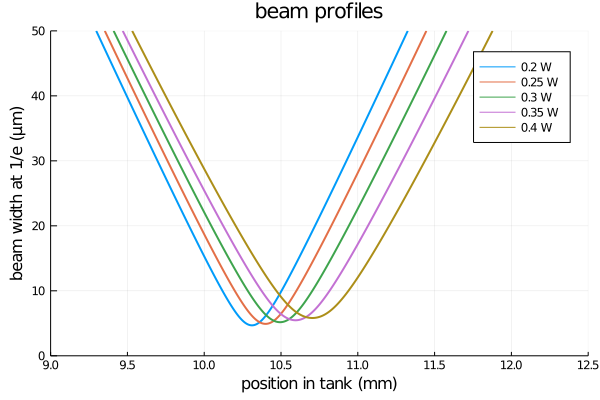
\includegraphics[width=0.8\textwidth]{./files/grinlensplots_profile.png}
\caption{
On voit ici le résultat de la simulation pour plusieurs puissances de laser. Comme attendu, plus la puissance est élevée, plus l'effet divergent est fort, et donc plus le waist est éloigné et large.
}
\end{figure}

On peut mesurer expérimentalement la position de cette largeur minimum du faisceau dans la fluorescine.

\begin{figure}
\centering
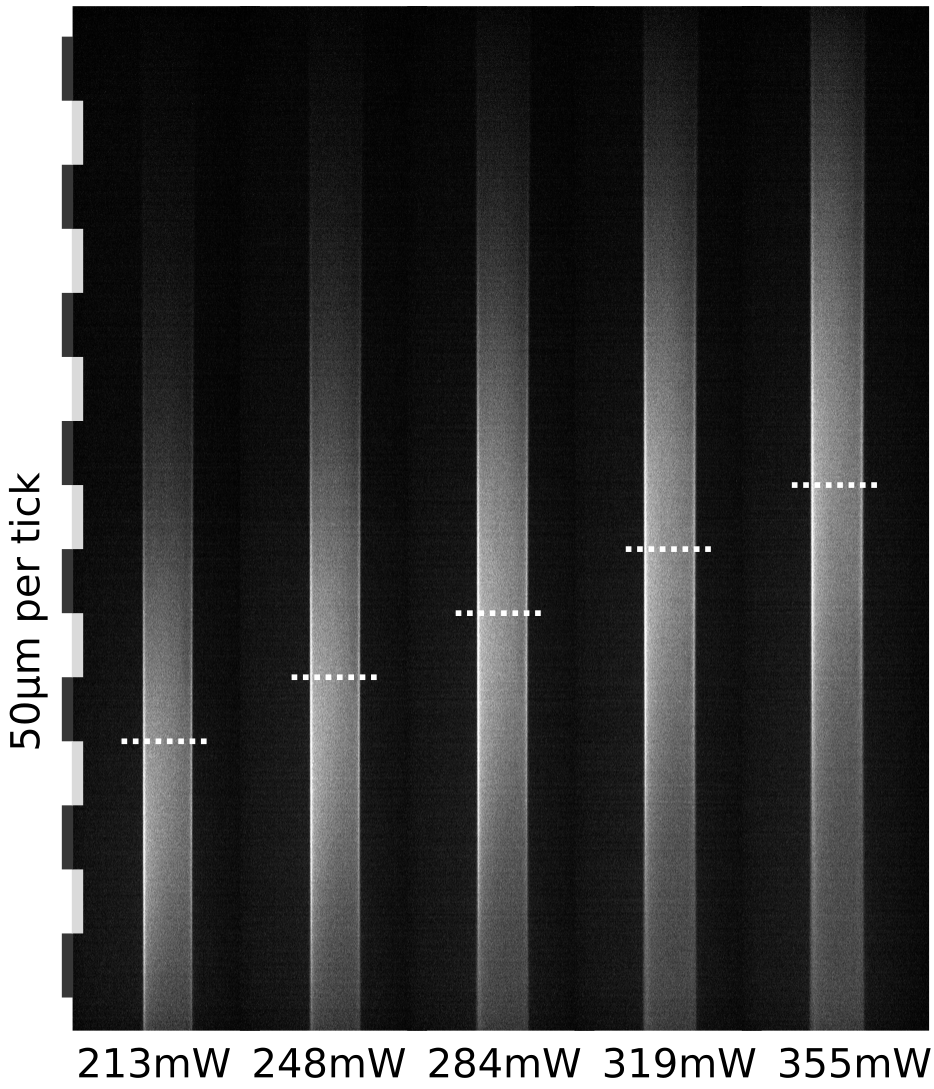
\includegraphics[width=0.8\textwidth]{./files/thermal-shift.svg.png}
\caption{
On voit ici une feuille de lumière imagée dans la fluorescéine pour plusieurs puissances laser différentes. La position du maximum d'intensité, et donc de la largeur minimale, est marquée par un trait en pointillé
}
\end{figure}

\begin{figure}
\centering
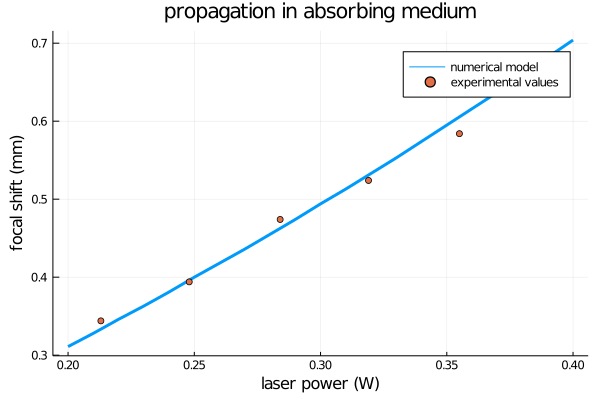
\includegraphics[width=0.8\textwidth]{./files/grinlensplots_model.png}
\caption{
voici la comparaison entre les données numériques et expérimentales
}
\end{figure}


\subsection{TODO analyse temporelle}
\chapter{Conclusion}\label{chapV}

% La compréhension du cerveau a longtemps reposé sur son étude statique d'une part sur sa découpe anatomique, qui a permis d'identifier des aires par leur forme (noyau, faisceau, strates...) et leur fonction, et d'autre part par sa composition cellulaire  Considérer le cerveau comme un assemblage de différents composants a permis de découvrir de nombreux mécanismes mais tous ces élements sont en réalité très interconnectés. Considérer le cerveau entier comme un système 

% Je suis nul pour écrire :(



Le cerveau a pendant longtemps été étudié par sa composition statique au niveau anatomique d'une part et cellulaire d'autre part. L'étude de son fonctionnement dynamique a été réalisée à ces deux échelles à l'aide des techniques IRM et électrophysiologie. Les nouvelles techniques d'imagerie appliquées au cerveau larves de poisson zèbre génétiquement modifiées permettent d'explorer une échelle intermédiaire nouvelle : le cerveau entier à la résolution du neurone. Cette échelle se prête particulièrement à l'étude de phénomènes impliquant un petit nombre de neurones distants les uns des autres. C'est notamment le cas de l'intégration multisensorielle.

Parmi les modèles d'intégration multisensorielle figure l'intégration visuo-vesti\-bulaire lors du contrôle postural. J'ai dans un premier temps reproduit cette boucle sensorimotrice dans un environnement de réalité virtuelle où la stimulation vestibulaire et l'environnement visuel sont en rétroaction sur les mouvements du poisson. Mes résultats suggèrent que la présence simultanée des deux modalités sensorielles améliore la qualité du contrôle postural par rapport à la présence d'une modalité seule.

Pour reproduire ces observations sous le microscope afin d'en comprendre les mécanismes neuronaux, plusieurs développements techniques étaient nécessaires. Il fallait d'une part construire un microscope à feuille de lumière capable d'enregistrer l'activité du cerveau lors d'une stimulation vestibulaire et d'autre part gagner le contrôle sur l'environnement visuel. Le premier point a été résolu par Geoffrey Migault avec un microscope à feuille de lumière rotatif permettant l'acquisition du cerveau lors d'une stimulation vestibulaire. Le second point a été résolu par Sébastien Wolf avec un microscope à feuille de lumière deux photons permettant l'acquisition du cerveau sans gêne pour le système visuel.

Combiner ces deux innovations a révélé plusieurs défis techniques : acheminer un laser deux photons dans une expérience en mouvement, maintenir une transmission et une polarisation suffisamment stable pour l'imagerie, s'affranchir des limites imposées par l'effet de lentille thermique dans un fluide en mouvement. Ces difficultés m'ont mené à m'intéresser à certains points que j'aborde dans ce manuscrit commes les propriétés de transmission des fibres optiques à cœur creux, aux conditions optimales d'impulsion pour un laser deux photons, à la théorie des lentilles thermiques. 

J'ai finalement obtenu un microscope permettant de réaliser l'acquisition un ou deux photons de l'activité neuronale pendant une stimulation vestibulaire en tangage et présente des cartes de réponse à une stimulation sinusoïdale. Ces cartes peuvent être comparées aux cartes équivalentes pour une stimulation en roulis et révèlent les mêmes zones d'activité, mais avec une temporalité différente. Mes expériences ne révèlent pas de différence notable entre les cartes en un ou deux photons.

Ce microscope ouvre la voix vers l'étude de l'intégration viso-vestibulaire lors du contrôle postural en tangage. Pour ce faire, il reste à adapter le système pour contrôler l'environnement virtuel et mettre en place la rétroaction permettant de reproduire les expériences de contrôle postural.
\appendix
\chapter{Appendice}\label{AppA}



% colors for code highlighting
\definecolor{mygreen}{RGB}{28,172,0}
\definecolor{mylilas}{RGB}{170,55,241}
\definecolor{deepblue}{rgb}{0,0,0.5}
\definecolor{deepred}{rgb}{0.6,0,0}
\definecolor{deepgreen}{rgb}{0,0.5,0}
\definecolor{lightgray}{rgb}{0.6,0.6,0.6}

% julia langage definition
\lstdefinelanguage{Julia}%
  {morekeywords={abstract,break,case,catch,const,continue,do,else,elseif,%
      end,export,false,for,function,immutable,import,importall,if,in,%
      macro,module,otherwise,quote,return,struct,switch,true,try,type,typealias,%
      using,while},%
   sensitive=true,%
   alsoother={\$,<:,::},%
   morecomment=[l]\#,%
   morecomment=[n]{\#=}{=\#},%
   morestring=[s]{"}{"},%
   morestring=[m]{'}{'},%
}[keywords,comments,strings]%

% general parameters for listings
\lstset{%
    breaklines          = true, %
    showstringspaces    = false,%
    basicstyle          = \ttfamily\small,
    % numbers=left, %
    % numberstyle={\tiny \color{black}},%
    frame               = leftline,%
    basewidth           = 0.45em,%
}
% MATLAB
\newcommand\matlabstyle{\lstset{%
    language=Matlab,%
    keywordstyle=\color{blue},%
    stringstyle=\color{mylilas},%
    commentstyle=\color{mygreen},%
    numberstyle={\small \color{black}},%
    numbersep=10pt, % 
    emph=[1]{classdef, for,end,break},emphstyle=[1]\color{red},%
}}
% PYTHON
\newcommand\pythonstyle{\lstset{%
    language=Python,%
    keywordstyle=\color{deepblue},%
    stringstyle=\color{deepgreen},%
    commentstyle=\color{lightgray},%
    otherkeywords={self},
}}
% JULIA
\newcommand\juliastyle{\lstset{%
    language         = Julia,
    keywordstyle     = \bfseries\color{blue},
    stringstyle      = \color{magenta},
    commentstyle     = \color{ForestGreen},
}}



% http://wiki.ljp.upmc.fr/zebrain/
% analyse en Julia






\section{Langage de programmation adapté}

\subsection{Memory mapping}

Du fait du volume des données traitées, notre processus d'analyse repose largement sur le \verb|memory mapping| comme solution de gestion des données brutes. Cela permet de traiter une portion de mémoire disque comme une portion de mémoire vive et ainsi de n'appliquer les opérations de chargement de données en mémoire vive qu'au moment de leur utilisation et de ne pas écrire systématiquement les opérations de lecture et d'écriture. Je compare ici les interfaces fournies dans les langages de programmation Matlab, Python, et Julia ainsi que la manière dont elles peuvent être étendues par des classes ou structures.

\subsubsection{Matlab}

La langage Matlab fournit la fonction \verb|memmapfile| (\href{https://fr.mathworks.com/help/matlab/ref/memmapfile.html}{doc}) qui permet de cartographier une zone mémoire contenant des données de type \verb|int8|, \verb|int16|, \verb|int32|, \verb|int64|, \verb|uint8|, \verb|uint16|, \verb|uint32|, \verb|uint64|, \verb|single|, ou \verb|double|.
J'ai implémenté plusieurs surcouches de la classe Matlab \verb|memmapfile| qui permettent de gérer l'accès à des données stockées sous différents formats comme le \verb|dcimg|, d'autre orientations que celle par défaut, et en utilisant l'indexation linéaire suivant (xy) en une seule ligne. Ces classes ont facilité l'écriture de code pour la manipulation des données brutes et aux différentes étapes de traitement, ainsi que des interfaces graphiques rudimentaires utilisées pour les visualiser mais ne permettent pas de profiter des optimisations de Matlab sur la vectorisation du calcul.
De plus, une gestion manuelle de la mémoire et des abstractions sur les tableaux de données manquent au langage pour que ces classes soit facilement réutilisables, ce qui conduit à de la duplication de code. Ci-dessous on peut voir la structure adoptée pour ces classes, qui surchargent les méthodes intégrées au langage \verb|subsref| et \verb|subsasgn|.


\matlabstyle
\begin{lstlisting}
classdef Mmap < handle
% the class Mmap is used to load a mmap of a binary file
% and redefine layers index when called as subscript
% subscript can be 4D or 3D

% [...] properties, contructor, and other methods definition

function out = subsref(self, S)        
    switch S(1).type
        case '()'
            new_S = self.subStruct(S);
            % [...] subscript manipulation
            out = subsref(self.mmap.Data.bit, new_S);
            % [...] returned data manipulation
            end
        case '.'
            out = builtin('subsref', self, S);
        otherwise
            error('subsref other than () or . not implemented')
    end        
end

end
\end{lstlisting}

\subsubsection{Python}

Le langage Python offre également une classe \verb|mmap| (\href{https://docs.python.org/3.8/library/mmap.html}{doc}) ainsi que sa bibliothèque Numpy avec la classe \verb|memmap| (\href{https://numpy.org/devdocs/reference/generated/numpy.memmap.html}{doc}). Une option \verb|order| permet de préciser l'ordre des données en mémoire, et donc d'adapter simplement la manière dont les données sont stockées à la manière donc elles seront utilisées. CaImAn implémente également une surcouche fine sur cette classe pour gérer ses conventions d'organisation de fichiers, où de nombreuses informations sont contenues dans le nom de fichier. J'en montre ci-dessous un extrait.

\pythonstyle
\begin{lstlisting}
def load_memmap(filename: str, mode: str = 'r') ->
    Tuple[Any, Tuple, int]:
    # [...]
    Yr = np.memmap(
        file_to_load,
        mode=mode,
        shape=prepare_shape((d1 * d2 * d3, T)),
        dtype=np.float32,
        order=order
        )
    if d3 == 1:
        return (Yr, (d1, d2), T)
    else:
        return (Yr, (d1, d2, d3), T)
\end{lstlisting}


\subsubsection{Julia}

Le langage Julia intègre un module dédié au \verb|memory mapping| (\href{https://docs.julialang.org/en/v1/stdlib/Mmap/index.html#Mmap.mmap}{doc}) qui permet d'accéder aux données par un objet qui se comporte de manière identique à un tableau Julia. Via le concept d'interfaces (\href{https://docs.julialang.org/en/v1/manual/interfaces/#man-interface-array-1}{doc}), en particulier l'interface de tableau, il est facile d'écrire une surcouche immédiatement compatible avec n'importe quelle fonction prenant en argument un tableau Julia. Cela est très différent de Matlab où il faut écrire des fonctions spécifiques et légèrement différent de Python où l'écriture de classes intermédiaires génère un surcoût important par rapport à Numpy. Je montre ici un exemple de surcouche mince sur la structure Julia \verb|mmap|.
Il est extrêmement facile de surcharger une telle classe Julia pour l'adapter à des usages différents sans avoir à en modifier le comportement. Par exemple, il suffit d'une dizaine de lignes pour rendre une telle structure compatible avec les données stockées sous le format de CaImAn tout en conservant la compatibilité avec d'autres formats, et pour un coût nul à l'exécution.
% Grâces aux interfaces, à la surcharge de méthodes, au filtrage par motif (\emph{pattern matching}, il est extrêmement facile de surcharger les méthodes d'un classe Julia pour l'adapter à des usages différents sans avoir à en modifier le comportement. Cela offre une souplesse précieuse lors du prototypage de même qu'en production dans des environnements différents. Par exemple, il suffit d'une dizaine de lignes pour rendre une telle structure compatible avec les données stockées sous le format de CaImAn tout en conservant la compatibilité avec d'autres formats, et pour un coût nul à l'exécution.

\juliastyle
\begin{lstlisting}
using Mmap

# ===== structure definition =====
struct Stack{T,N} <: AbstractArray{T,N}
    file::String        # path plus filename of raw raster file
    dims::NTuple{N,Int} # N integers correspondig to dimension sizes
    space::String       # e.g. RAST
    m::Array{T,N}       # memory mapped array
    # core constructor
    Stack(file::String, T::DataType, dims::NTuple, space::String) =
      new{T,length(dims)}(file, dims, space,
        Mmap.mmap(open(file), Array{T, length(dims)}, dims))
end

# [...] more methods like constructor overload

# ===== interface implementation =====
# following functions allows to access Stack like an Array
Base.size(S::Stack) = S.dims
# linear indexing
Base.getindex(S::Stack, i::Int) = S.m[i] 
# cartesian indexing
Base.getindex(S::Stack{T,N}, I::Vararg{Int, N}) where {T,N} = S.m[I...]
\end{lstlisting}


% \subsection{Vitesse d'exécution}
% \subsection{Gestion et maintenance du code}



\subsection{Function broadcasting}

% TODO
\backmatter

\cleardoublepage
\phantomsection
\addcontentsline{toc}{chapter}{Bibliographie}
%% reference style
\bibliographystyle{./bib/thesefr-href}
\bibliography{./bib/zotero}

%%% LOOK to be replaced by, for final version:
%\intput{these.bbl}

%%% LOOK 4th COVER %%%
% \backcover % requires thcover.sty loaded and thcoverdata.tex filled
\end{document}